%%%%%%%%%%%%%%%%%%%%%%%%%%%%%%%%%%%%%%%%%
% Masters/Doctoral Thesis 
% LaTeX Template
% Version 2.5 (27/8/17)
%
% This template was downloaded from:
% http://www.LaTeXTemplates.com
%
% Version 2.x major modifications by:
% Vel (vel@latextemplates.com)
%
% This template is based on a template by:
% Steve Gunn (http://users.ecs.soton.ac.uk/srg/softwaretools/document/templates/)
% Sunil Patel (http://www.sunilpatel.co.uk/thesis-template/)
%
% Template license:
% CC BY-NC-SA 3.0 (http://creativecommons.org/licenses/by-nc-sa/3.0/)
%
%%%%%%%%%%%%%%%%%%%%%%%%%%%%%%%%%%%%%%%%%

%----------------------------------------------------------------------------------------
%	PACKAGES AND OTHER DOCUMENT CONFIGURATIONS
%----------------------------------------------------------------------------------------

\documentclass[
11pt, % The default document font size, options: 10pt, 11pt, 12pt
%oneside, % Two side (alternating margins) for binding by default, uncomment to switch to one side
english, % ngerman for German
singlespacing, % Single line spacing, alternatives: onehalfspacing or doublespacing
%draft, % Uncomment to enable draft mode (no pictures, no links, overfull hboxes indicated)
%nolistspacing, % If the document is onehalfspacing or doublespacing, uncomment this to set spacing in lists to single
%liststotoc, % Uncomment to add the list of figures/tables/etc to the table of contents
%toctotoc, % Uncomment to add the main table of contents to the table of contents
%parskip, % Uncomment to add space between paragraphs
%nohyperref, % Uncomment to not load the hyperref package
headsepline, % Uncomment to get a line under the header
%chapterinoneline, % Uncomment to place the chapter title next to the number on one line
%consistentlayout, % Uncomment to change the layout of the declaration, abstract and acknowledgements pages to match the default layout
]{MastersDoctoralThesis} % The class file specifying the document structure

% \usepackage{graphicx}
% \usepackage{subcaption}


\usepackage[utf8]{inputenc} % Required for inputting international characters
\usepackage[T1]{fontenc} % Output font encoding for international characters
\usepackage{rotating}
\usepackage{chemformula}

\usepackage{mathpazo} % Use the Palatino font by default
\usepackage{outlines}
%\usepackage[backend=bibtex,style=authoryear,natbib=true]{biblatex} % Use the bibtex backend with the authoryear citation style (which resembles APA)
\usepackage[style=numeric-comp, labelnumber, backend=biber,natbib=true]{biblatex}

\DeclareNameAlias{sortname}{family-given}

\DeclareFieldFormat{labelnumberwidth}{#1.}
\defbibenvironment{bibliography}
  {\list
    {\printtext[labelnumberwidth]{%
        \printfield{labelprefix}%
        \printfield{labelnumber}}}
    {\setlength{\labelwidth}{\labelnumberwidth}%
      \setlength{\leftmargin}{\labelwidth}%
      \setlength{\labelsep}{\biblabelsep}%
      \addtolength{\leftmargin}{\labelsep}%
      \setlength{\itemsep}{\bibitemsep}%
      \setlength{\parsep}{\bibparsep}}%
      \renewcommand*{\makelabel}[1]{\hss##1}}
  {\endlist}
  {\item}

%\usepackage[sort, numbers]{natbib}
\usepackage{float}
% \addbibresource{Refrences/example.bib} % The filename of the bibliography
\addbibresource{Refrences/related_work.bib} % The filename of the bibliography
\addbibresource{Refrences/datasets.bib} % The filename of the bibliography
\addbibresource{Refrences/sne.bib} % The filename of the bibliography
\addbibresource{Refrences/tools.bib} % The filename of the bibliography
 
\usepackage[autostyle=true]{csquotes} % Required to generate language-dependent quotes in the bibliography

\usepackage{amssymb}
\usepackage{multirow}
\usepackage{adjustbox}
\usepackage{tabularx}

%\usepackage[demo]{graphicx}
\usepackage{subcaption}

% for arrays 
\usepackage{tikz}

% for graph trees
\usepackage{qtree}

\usetikzlibrary{calc}

\DeclareCiteCommand*{\citetitle}%your new citecommand \citetitle*
  {\boolfalse{citetracker}%
   \boolfalse{pagetracker}%
   \usebibmacro{prenote}}
  {\ifciteindex
     {\indexfield{indextitle}}
     {}%
    \printtext[bibhyperref]{\printfield[citetitle]{labeltitle}}}%like \citetile, 
    %only added \printtext[bibhyperref]{...} in this line
  {\multicitedelim}
  {\usebibmacro{postnote}}

\DeclareCiteCommand*{\citeyear}%your new citecommand \citetitle*
  {\boolfalse{citetracker}%
   \boolfalse{pagetracker}%
   \usebibmacro{prenote}}
  {\ifciteindex
     {\indexfield{indextitle}}
     {}%
    \printtext[bibhyperref]{[\printfield[citefield]{labelnumber}]}}%like \citetile, 
    %only added \printtext[bibhyperref]{...} in this line
  {\multicitedelim}
  {\usebibmacro{postnote}}



%----------------------------------------------------------------------------------------
%	MARGIN SETTINGS
%----------------------------------------------------------------------------------------

\geometry{
	paper=a4paper, % Change to letterpaper for US letter
	inner=2.5cm, % Inner margin
	outer=3.8cm, % Outer margin
	bindingoffset=.5cm, % Binding offset
	top=1.5cm, % Top margin
	bottom=1.5cm, % Bottom margin
	%showframe, % Uncomment to show how the type block is set on the page
}

%----------------------------------------------------------------------------------------
%	THESIS INFORMATION
%----------------------------------------------------------------------------------------

\thesistitle{Development and Analysis of new Activation Based Load Profiles} % Your thesis title, this is used in the title and abstract, print it elsewhere with \ttitle
\supervisor{doc. dr. Marko \textsc{Meža} and \\ Dr. Carolina \textsc{Fortuna}} % Your supervisor's name, this is used in the title page, print it elsewhere with \supname
\examiner{} % Your examiner's name, this is not currently used anywhere in the template, print it elsewhere with \examname
\degree{Masters of Electrical Engineering} % Your degree name, this is used in the title page and abstract, print it elsewhere with \degreename
\author{Jakob \textsc{Jenko, BSc}} % Your name, this is used in the title page and abstract, print it elsewhere with \authorname
\addresses{} % Your address, this is not currently used anywhere in the template, print it elsewhere with \addressname

\subject{Data science} % Your subject area, this is not currently used anywhere in the template, print it elsewhere with \subjectname
\keywords{load profiling, energy data, energy saving, dimensionality reduction, elderly care, anomaly detection} % Keywords for your thesis, this is not currently used anywhere in the template, print it elsewhere with \keywordnames
\slokeywords{profiliranje porabe, energetski podatki, učinkovita poraba, zmanjšanje dimenzionalnosti, oskrba starejših, zaznavanje anomalij} % Keywords for your thesis, this is not currently used anywhere in the template, print it elsewhere with \slokeywordnames

\university{\href{https://www.uni-lj.si}{University of Ljubljana}} % Your university's name and URL, this is used in the title page and abstract, print it elsewhere with \univname
\department{\href{http://department.university.com}{}} % Your department's name and URL, this is used in the title page and abstract, print it elsewhere with \deptname
\group{\href{http://researchgroup.university.com}{}} % Your research group's name and URL, this is used in the title page, print it elsewhere with \groupname
\faculty{\href{https://www.fe.uni-lj.si}{Faculty of Electical Engineering}} % Your faculty's name and URL, this is used in the title page and abstract, print it elsewhere with \facname

\AtBeginDocument{
\hypersetup{pdftitle=\ttitle} % Set the PDF's title to your title
\hypersetup{pdfauthor=\authorname} % Set the PDF's author to your name
\hypersetup{pdfkeywords=\keywordnames} % Set the PDF's keywords to your keywords
\hypersetup{pdfkeywords=\slokeywordnames} % Set the PDF's keywords to your keywords
}

\begin{document}

\frontmatter % Use roman page numbering style (i, ii, iii, iv...) for the pre-content pages

\pagestyle{plain} % Default to the plain heading style until the thesis style is called for the body content

%----------------------------------------------------------------------------------------
%	TITLE PAGE
%----------------------------------------------------------------------------------------

\begin{titlepage}
\begin{center}

\vspace*{.06\textheight}
{\scshape\LARGE \univname\par}\vspace{1.5cm} % University name
\textsc{\Large Master’s Thesis}\\[0.5cm] % Thesis type

\HRule \\[0.4cm] % Horizontal line
{\huge \bfseries \ttitle\par}\vspace{0.4cm} % Thesis title
\HRule \\[1.5cm] % Horizontal line
 
\begin{minipage}[t]{0.4\textwidth}
\begin{flushleft} \large
\emph{Author:}\\
\href{}{\authorname} % Author name - remove the \href bracket to remove the link
\end{flushleft}
\end{minipage}
\begin{minipage}[t]{0.4\textwidth}
\begin{flushright} \large
\emph{Mentors:} \\
\href{}{\supname} % Supervisor name - remove the \href bracket to remove the link  
\end{flushright}
\end{minipage}\\[3cm]
 
\vfill

\large \textit{A thesis submitted in fulfillment of the requirements\\ for the degree of \degreename}\\[0.3cm] % University requirement text

 
\vfill

{\large \today}\\[4cm] % Date
% \includegraphics{Logo} % University/department logo - uncomment to place it
 
\vfill
\end{center}
\end{titlepage}

%----------------------------------------------------------------------------------------
%	DECLARATION PAGE
%----------------------------------------------------------------------------------------

% \begin{declaration}
% \addchaptertocentry{\authorshipname} % Add the declaration to the table of contents
% \noindent I, \authorname, declare that this thesis titled, \enquote{\ttitle} and the work presented in it are my own. I confirm that:

% \begin{itemize} 
% \item This work was done wholly or mainly while in candidature for a research degree at this University.
% \item Where any part of this thesis has previously been submitted for a degree or any other qualification at this University or any other institution, this has been clearly stated.
% \item Where I have consulted the published work of others, this is always clearly attributed.
% \item Where I have quoted from the work of others, the source is always given. With the exception of such quotations, this thesis is entirely my own work.
% \item I have acknowledged all main sources of help.
% \item Where the thesis is based on work done by myself jointly with others, I have made clear exactly what was done by others and what I have contributed myself.\\
% \end{itemize}

 
% \noindent Signed:\\
% \rule[0.5em]{25em}{0.5pt} % This prints a line for the signature
 
% \noindent Date:\\
% \rule[0.5em]{25em}{0.5pt} % This prints a line to write the date
% \end{declaration}


\cleardoublepage

%----------------------------------------------------------------------------------------
%	QUOTATION PAGE
%----------------------------------------------------------------------------------------

\vspace*{0.2\textheight}

\noindent\enquote{\itshape In science, great oaks grow from little acorns.}\bigbreak

\hfill D. Everett 

% %----------------------------------------------------------------------------------------
% %	DISPOSITION PAGE 
% %----------------------------------------------------------------------------------------


% %----------------------------------------------------------------------------------------
% %	ABSTRACT PAGE
% %----------------------------------------------------------------------------------------

\begin{abstract}
\addchaptertocentry{\abstractname} % Add the abstract to the table of contents
This work explores the potential of electrical energy data
and how load profiles can be used to address issues such as the optimization of electrical energy consumption patterns and the aging population.
The efficient presentation of energy data through load profiles is a constant narrative throughout the thesis.
Optimizing consumption has the potential to significantly reduce the human footprint
since a third of electrical energy in the EU is consumed in the residential sector.
Furthermore, we utilize load profiles to address issues such as the aging population. 
We developed an elderly care assisted living system to detect anomalies in the usage patterns of the elderly.
The system identifies accidents such as falls, strokes, or dementia-induced altered behavior.

We performed a comprehensive review of existing publications and use-cases.
These publications were mapped into a table, which revealed gaps in the load profiles that were not yet researched or used.
Next, we analyzed the load profiles and using t-SNE presented how profiles are related in high dimensional space. 

With the successful implementation of the elderly care system, we confirmed that unused load profiles are applicable.
The findings of this thesis showcase the untapped potential of energy data where the table of profiles provides a foundation for further research in this area.

\par
\par\textbf{Keywords}: \keywordnames 

\end{abstract}

% %----------------------------------------------------------------------------------------
% %	SLO ABSTRACT PAGE
% %----------------------------------------------------------------------------------------

\begin{sloabstract}
  \addchaptertocentry{\sloabstractname} % Add the abstract to the table of contents
  
  V tem delu raziščemo možnost uporabe profilov porabe električne energije za naslavljaje ovir samostojnega bivanja starejšega prebivalstva in za optimizacijo porabe električne energij. 
  Osrednja tema magistrske naloge je učinkovita predstavitev podatkov s pomočjo profilov uporabe.
  Optimizacija porabe energije lahko bistveno zmanjša ogljični odtis človeka, saj se v EU tretjina električne energije porabi v stanovanjskem sektorju.

  Opravili smo obsežen pregled obstoječih publikacij in primerov uporabe.
  Publikacije smo prikazali v tabeli, ki je razkrila vrzeli profilov, ki še niso bili raziskani ali uporabljeni.
  Nato smo analizirali profile obremenitve in s pomočjo t-SNE predstavili, kako so profili povezani v visokodimenzionalnem prostoru. 
  Z novo prodobljenim znanjem smo razvili smo sistem za oskrbo starejših, ki lahko pomaga podaljšati samosotjno bivanje starejših oseb.
  Sistem preko analize profilov porabe elektične energije prepozna anomalije, kot so padci, kapi ali spremenjeno vedenje zaradi demence.

  Z uspešno implementaacijo sistema za oskrbo starejših smo potrdili, da so neuporabljeni profili uporabni.
  Ugotovitve te magistrske naloge prikazujejo neizkoriščen potencial podatkov o energiji, kjer tabela profilov predstavlja osnovo za nadaljnje raziskave na tem področju.
  
  \par
  \par\textbf{Ključne besede}: \slokeywordnames 

  \end{sloabstract}

% %----------------------------------------------------------------------------------------
% %	ACKNOWLEDGEMENTS
% %----------------------------------------------------------------------------------------

\begin{acknowledgements}
\addchaptertocentry{\acknowledgementname} % Add the acknowledgements to the table of contents
I would like to thank the following people without whom this thesis would not be possible.
Dr. Carolina Fortuna and Dr. Marko Meža helped me with the research, by providing continuous feedback and support.
The scientific and open-source community provided the data and the tools used throughout the thesis.
Friends and colleagues, who through discussion helped induce the ideas that were put forward through the thesis. 
My family, who inspired, supported and encouraged me to pursue my studies in the first place.
And my partner Nika, who supported me through all my years of studies in all aspects possible.

\end{acknowledgements}

% %----------------------------------------------------------------------------------------
% %	LIST OF CONTENTS/FIGURES/TABLES PAGES
% %----------------------------------------------------------------------------------------

\tableofcontents % Prints the main table of contents

\listoffigures % Prints the list of figures

\listoftables % Prints the list of tables

% %----------------------------------------------------------------------------------------
% %	ABBREVIATIONS
% %----------------------------------------------------------------------------------------

\begin{abbreviations}{ll} % Include a list of abbreviations (a table of two columns)

\textbf{LP} & \textbf{L}oad \textbf{P}rofile \\
\textbf{TP} & \textbf{T}able of load \textbf{P}rofiles \\
\textbf{P} & \textbf{P}ower (profile) \\
\textbf{A} & \textbf{A}ctivation (profile) \\
\textbf{ZEB} & \textbf{Z}ero \textbf{E}nergy \textbf{B}uilding \\
\textbf{DR} & \textbf{D}emand \textbf{R}esponse \\
\textbf{AD} & \textbf{A}nomaly \textbf{D}etection \\
\textbf{EC} & \textbf{E}lderly \textbf{C}are \\
\textbf{DER} & \textbf{D}istributed \textbf{E}nergy \textbf{R}esources \\
\textbf{HVAC} & \textbf{H}eating, \textbf{V}entilation and \textbf{A}ir \textbf{C}onditioning\\
\textbf{EV} & \textbf{E}lectric \textbf{V}ehiecle \\
\textbf{PV} & \textbf{P}hoto \textbf{V}oltaics \\
\textbf{EU} & \textbf{E}uropean \textbf{U}nion \\
\textbf{NILM} & \textbf{N}on \textbf{I}ntrusive \textbf{L}oad \textbf{M}onitoring\\
\textbf{t-SNE} & \textbf{t}-distributed \textbf{s}tochastic \textbf{n}eighbor \textbf{e}mbedding\\
\textbf{PCA} & \textbf{P}rincipal \textbf{C}omponent \textbf{A}nalysis \\
\textbf{EDA} & \textbf{E}xploratory \textbf{D}ata \textbf{A}nalysis \\

\end{abbreviations}

% %----------------------------------------------------------------------------------------
% %	PHYSICAL CONSTANTS/OTHER DEFINITIONS
% %----------------------------------------------------------------------------------------

% \begin{constants}{lr@{${}={}$}l} % The list of physical constants is a three column table

% The \SI{}{} command is provided by the siunitx package, see its documentation for instructions on how to use it

% Speed of Light & $c_{0}$ & \SI{2.99792458e8}{\meter\per\second} (exact)\\
%Constant Name & $Symbol$ & $Constant Value$ with units\\

%\end{constants}

% %----------------------------------------------------------------------------------------
% %	SYMBOLS
% %----------------------------------------------------------------------------------------

% \begin{symbols}{lll} % Include a list of Symbols (a three column table)

% $a$ & distance & \si{\meter} \\
% $P$ & power & \si{\watt} (\si{\joule\per\second}) \\
% Symbol & Name & Unit \\

% \addlinespace % Gap to separate the Roman symbols from the Greek

% $\omega$ & angular frequency & \si{\radian} \\

% \end{symbols}

% %----------------------------------------------------------------------------------------
% %	DEDICATION
% %----------------------------------------------------------------------------------------

% \dedicatory{Dedicated to the scientific community\ldots} 

% %----------------------------------------------------------------------------------------
% %	THESIS CONTENT - CHAPTERS
% %----------------------------------------------------------------------------------------

\mainmatter % Begin numeric (1,2,3...) page numbering

\pagestyle{thesis} % Return the page headers back to the "thesis" style

% % Include the chapters of the thesis as separate files from the Chapters folder
% % Uncomment the lines as you write the chapters

\chapter{Introduction}
\label{chapter1}

Climate change calls for a shift to renewable energy and restructuring of the electric power industry.
Source \cite{eurostat2020} shows that as of the time of reading this paper, 44 \% of produced electricity in Europe was from combustible sources such as gas, fuel, and coal. Even 
though that is a significant decrease of 10 \% in the last 10 years, it is a significant carbon dioxide emitter.
The same source \cite{eurostat2020} also states that a third of energy is consumed by the residential sector. It is estimated, 
that the human population will reach 10 billion inhabitants in the next 10 years, and ever-increasing ownership of electrical appliances such as smartphones, HVACs, and EVs will further elevate this issue.
Acknowledging this, reducing consumption in the residential sector could leave a significant impact on the human footprint. 

%increased time spent indoors*

The EU aims to be climate neutral by 2050, therefore it seeks to improve the efficiency of every part of pollution contributors through The European Green Deal.
A large part of these contributors is the Energy sector.
A subpart of the energy sector is the residential sector, where many advancements could be made to help to reach the goal.  

This could be achieved through various applications and methods that use load profiling as their core technology.
Authors in paper \cite{Chuan2014} proposed a method to reduce peak loads by studying consumer
appliance usage patterns. Paper \cite{Csoknyai2019} studied consumer usage patterns, and returned feedback that contributed to reducing consumption.
Another notable way is the use of distributed energy resources and managing them in such a way as to decrease the net output of energy flow such as the authors describe in
\cite{MORENOJARAMILLO2021445}. All described methods would reduce and alleviate the load off the power grid.

Load profiling in building energy consumption is not a novelty and had been in research since the 1980s.
While it was thought that aggregated LPs of households are relatively predictable, recent data obtained using smart meter data showed large deviance from user to user due to different lifestyles, as the author states in paper \cite{Review2021}.
In recent years LPs have changed due to renewable energy accelerated development of distributed energy resources such as residential photovoltaic
power plants, home wind energy, and using EVs with home batteries. Socioeconomic changes such as work-from-home, also drastically reshaped the LP curve. 

The thesis aims to propose and develop new, previously unused LPs, that will contribute to mitigating the raised issues.
Presenting consumption with the right LPs, will help dwellers be more aware of their consumption and in terms increase their energy efficiency.
Energy efficiency is the basis of our research, throughout the thesis we will explore LPs that were not yet utilized.
We will perform an EDA to make sense of what they are, and what information they contain.
This obtained knowledge will be used in a practical use-case to showcase that these profiles can be effectively utilized.
We will design an elderly care assisted living monitoring system to detect anomalies in consumption patterns to detect strokes and falls.

Before we fully disclose our contributions, let us first have an overview of what LPs are and in which other use cases they can be utilized, besides the ones just mentioned.

% finishing words here 

\section{Definition and Types of LPs}
\label{sec:LP_types}
Author Proedrou \cite{Review2021} defines terms as follows:

% definiton
% usage
% analysis

\begin{itemize}
	\item Load: the electricity that all electricity-powered devices in the household consume in unit time.
	\item Profile: a graph representing the significant features of the electricity load over time.
\end{itemize}

In other words, LPs are a graphical presentation of the consumption features of a building over time. 
Here, features could be anything that presents consumption. 
In most cases that is electrical power, measured in kilowatts.
The time range used to present the consumption could be anything from daily, weekly, monthly to yearly.

One thing to mention here is, that although the buildings were mostly consuming energy in the past, nowadays, they also produce it.
While this may slightly alter the definition of LPs, it has also made them more useful, as they can now be used to depict both energy consumption and production.
Throughout this thesis, we primarily focus on the use of load profiles to represent electricity consumption, but it's important to consider their potential for presenting energy production as well.

\subsection{Feature Set} 
\label{ssec:feature_set}

To identify the fundamental features of energy consumption in buildings, we need to examine the way that consumption is typically measured.
Three main features allow us to determine the amount of energy being used by a user:

\begin{figure}[H]
  \Tree[.base\ features [.power ]
          [.timestamp ]
          [.name ]
                ]
\end{figure}

If we translate these features to the time domain and observe them over a specified amount of time, new features emerge. 
The most notable example is the observation of electrical power over one hour.
This results in the amount of energy consumed often referred to as energy $E$, which is one of the most common ways used to bill a customer for his power consumption.

We can also extract features such as the number of activations or time of operation for each activation.
This can be done using sensors to detect activity or even extract this from power consumption data.
In cases where we are observing individual appliances, this can be done using simple signal processing techniques.
In cases where we are observing buildings, this could be achieved using more complex disaggregation algorithms also known as NILM (non-intrusive load monitoring) algorithms.
NILM algorithms enable us to detect consumption patterns of multiple appliances from a single power meter.

% Time domain
\begin{figure}[H]
  \Tree[.time\ domain\ features [.energy $E$ ]
          [.number\ of\ activations $N_{act}$  ]
          [.operating\ time $t_{oper}$  ]
                ]
\end{figure}

\begin{figure}[H]
	\centering
	\caption{Simple signal processing of power consumption for a single appliance}
	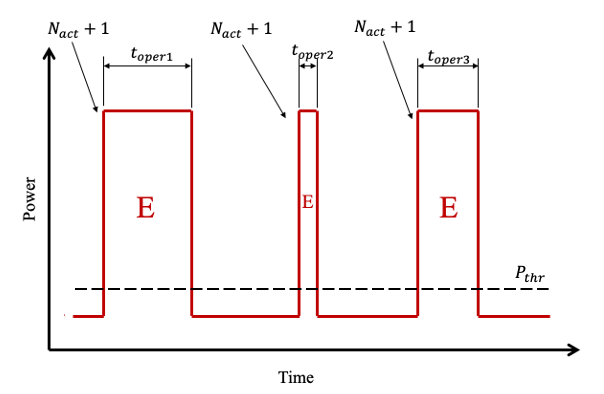
\includegraphics[width=0.9\textwidth]{Figures/profile_sketches/singal_processing_thr.png}
	\label{fig:sig_proc_fig}
\end{figure}

As we can see in Figure \ref{fig:sig_proc_fig} all three time-domain features can be extracted from the graphical presentation.
The amount of energy consumed, denoted as $E$, is equal to the area under the graphical presentation or in other words integral of power over time. 
The number of activations, denoted as $N_{act}$, can be measured based on the number of times the power value exceeded some pre-defined threshold $P_{thr}$. 
The time between on and off events is denoted as $t_{oper}$, where we use the same threshold as with $N_{act}$.
While there are other features, such as time between activations, or total operational time that could be
extracted, these are not commonly used in related work.

% \begin{figure}[H]
% \Tree[.frequency\ domain\ features [.Operation\ Modes ]]
% \end{figure}
% The same as we can present power in the time domain, the same can be done in the frequency domain. 
% One actual example can be seen in Figure \ref{fig:freq}.
% Here, it is hard to extract more features, but one possibility could be
% detecting the number of operation modes based on the number of peaks, using signal processing algorithms.

% \begin{figure}[H]
% 	\centering
% 	\caption{Frequency of power values for the toaster. Actual data from the REFIT dataset.}
% 	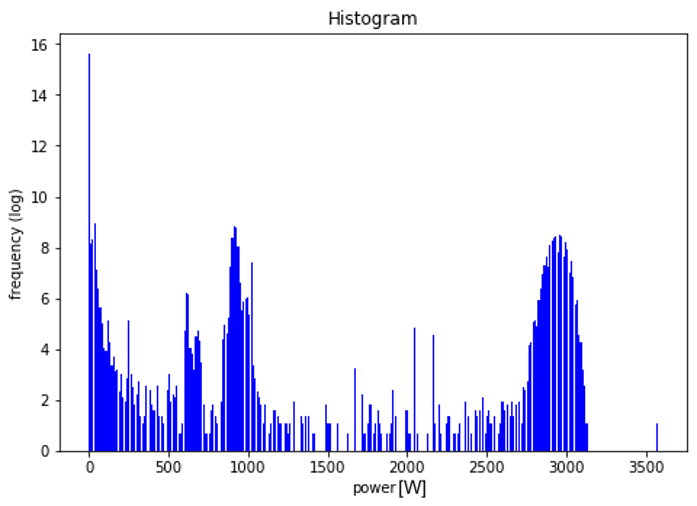
\includegraphics[width=0.9\textwidth]{Figures/profile_sketches/freq.png}
% 	\label{fig:freq}
% \end{figure}

% In the case of Figure \ref{fig:freq} we are observing a toaster over one year.
% Toasters are usually simple appliances using a heating element and a thermostat, meaning that the power consumption should be constant and set by the resistance of the heating element.
% The Figure shows \ref{fig:freq} a nice normal distribution of power values around 3 kW, 
% which we can assume is the heating element.
% We can notice two other peaks one at roughly 1 kW and the other at 0.7 kW.
% Since toasters usually do not have operation modes, we could assume that there 
% are other appliances plugged into the metering device, 
% meaning this could be a use-case for this kind of LP.

\subsection{Types of LPs} 

\subsubsection{Power LP}
\label{ssec:feature_set}

Combinations of the features result in many possible types of LPs that enable us to present the data.
The most commonly used type of LP is average power consumption over some time.
One such example can be seen in Figure \ref{fig:daily_power_profile}. 
Here, we used daily timescale, since it is so commonly used, it is also known as the standard daily LP. 
It can be used to portray per-building as well as per-appliance data.
It is one of the most versatile LPs, and it is used in fields such as demand response, anomaly detection and zero-energy buildings.
While the LP in Figure \ref{fig:daily_power_profile} is a sketch, it still presents consumption trends in morning and evening peaks.
% ad usage and then analysis
\begin{figure}[H]
	\centering
	\caption{Average daily usage profile for an appliance or a building}
	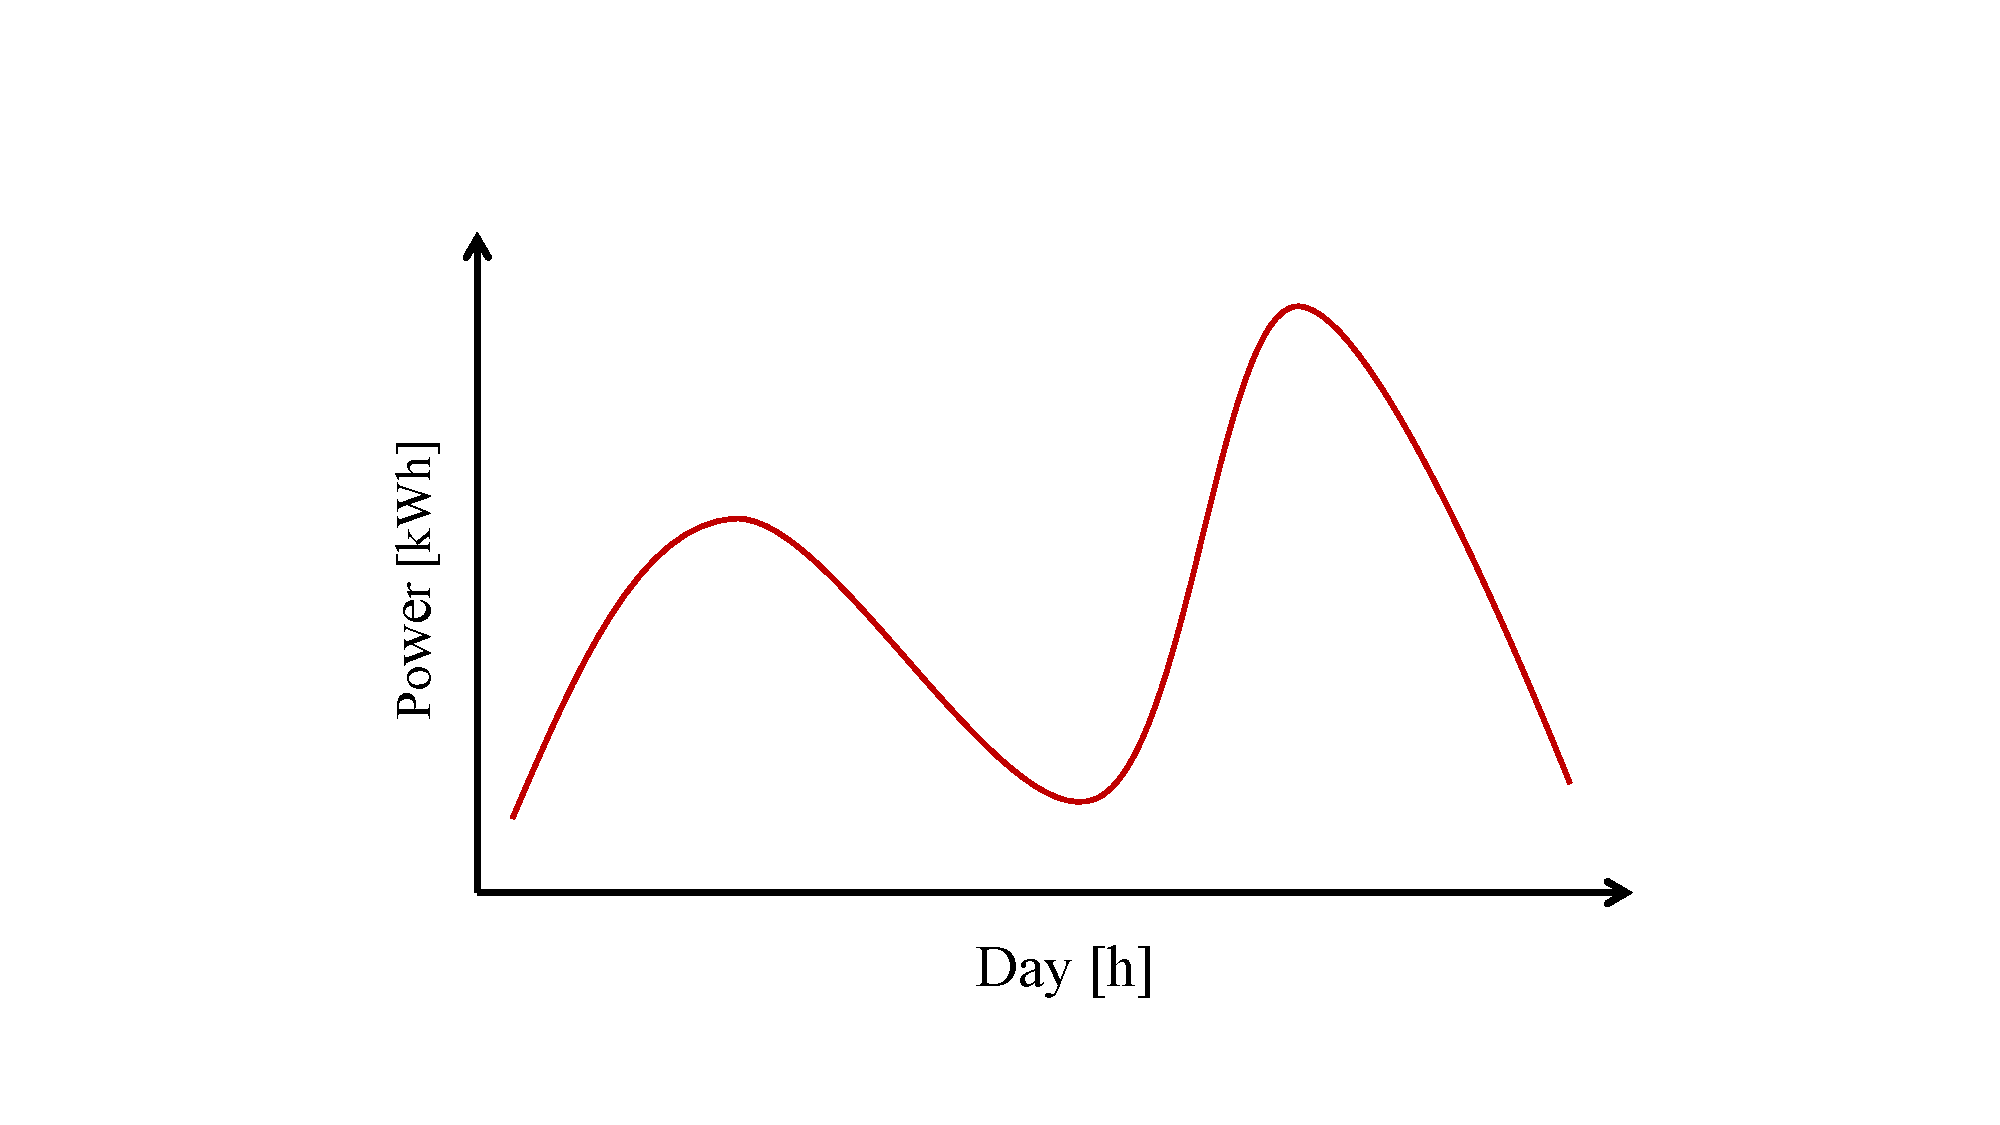
\includegraphics[width=0.9\textwidth]{Figures/profile_sketches/slide1.pdf}
	\label{fig:daily_power_profile}
\end{figure}

\subsubsection{Activation LP}
Alternatively, we can use a histogram-based presentation to present a number of activations feature such as can be seen in Figure \ref{fig:daily_act_profile}.
Here, we split the given timescale into discrete intervals also known as buckets. 
These buckets are then filled with activations that had taken place in a given interval. 
In the case of Figure, \ref{fig:daily_act_profile} timescale is a day, and it was split into 12 intervals.
While this is not real-world data, we can still observe consumption patterns throughout the day with morning and evening peaks. 
Activation LP is usually used to portray per-appliance data. 
In order to portray per-building data, we would need to install a power meter for every appliance in the building.
This LP has the very same use-cases as the power type and can be used in the same fields, but as mentioned, it is less practical for per-building LPs.
While Figure \ref{fig:daily_act_profile} presents the same data as Figure \ref{fig:daily_power_profile},
due to data processing, it could potentially reveal more relevant consumption patterns.
The downside is that we have to invest additional time to process power data into activations.

\begin{figure}[H]
	\centering
	\caption{Histogram of daily activations profile for an appliance or a building}
	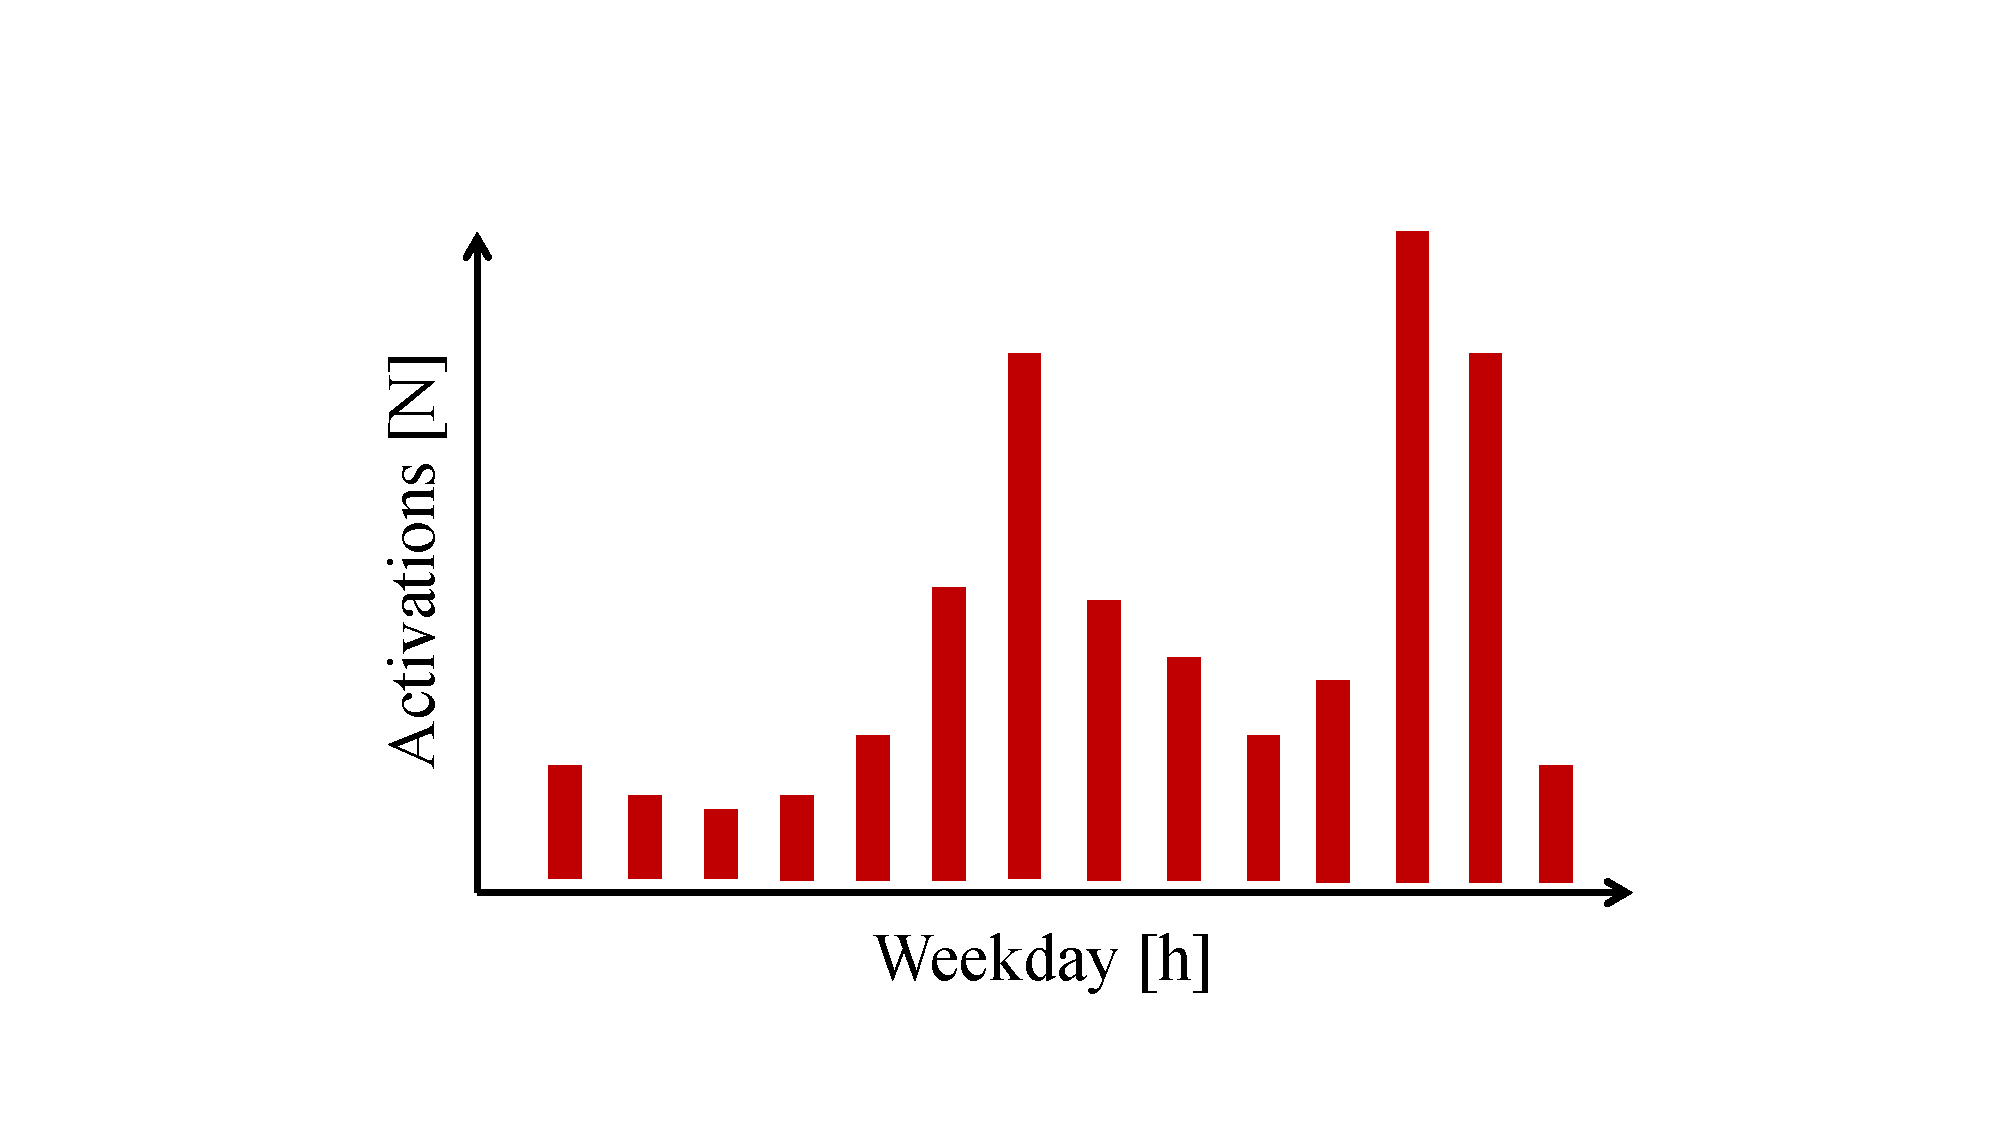
\includegraphics[width=0.9\textwidth]{Figures/profile_sketches/slide5.pdf}
	\label{fig:daily_act_profile}
\end{figure}

\subsubsection{Per-Building Per-Appliance LP}
The next two types of LP, known as per-building per-appliance LPs, can be used to present both whole-building usage and per-appliance consumption.
Figure \ref{fig:daily_act_m_profile} and \ref{fig:daily_power_m_profile} provide two such examples.
In the case of activation LP, we concatenate activations of each appliance and label them accordingly.
This approach enables us to see the contribution of each appliance to the total number of activations in each bucket.
The per-building per-appliance LPs hold the potential to be used in the same fields as the first two types, but practically they are primarily used in demand response.
This additional information enables us to better understand the data and potentially discover patterns that we otherwise would not be able to.
%The reason behind slow adoption could be that this additional information is not needed.

\begin{figure}[H]
	\begin{subfigure}{.5\textwidth}
		% \centering
		\caption{Daily per-building per-appliance activations LP for appliances A and B}
		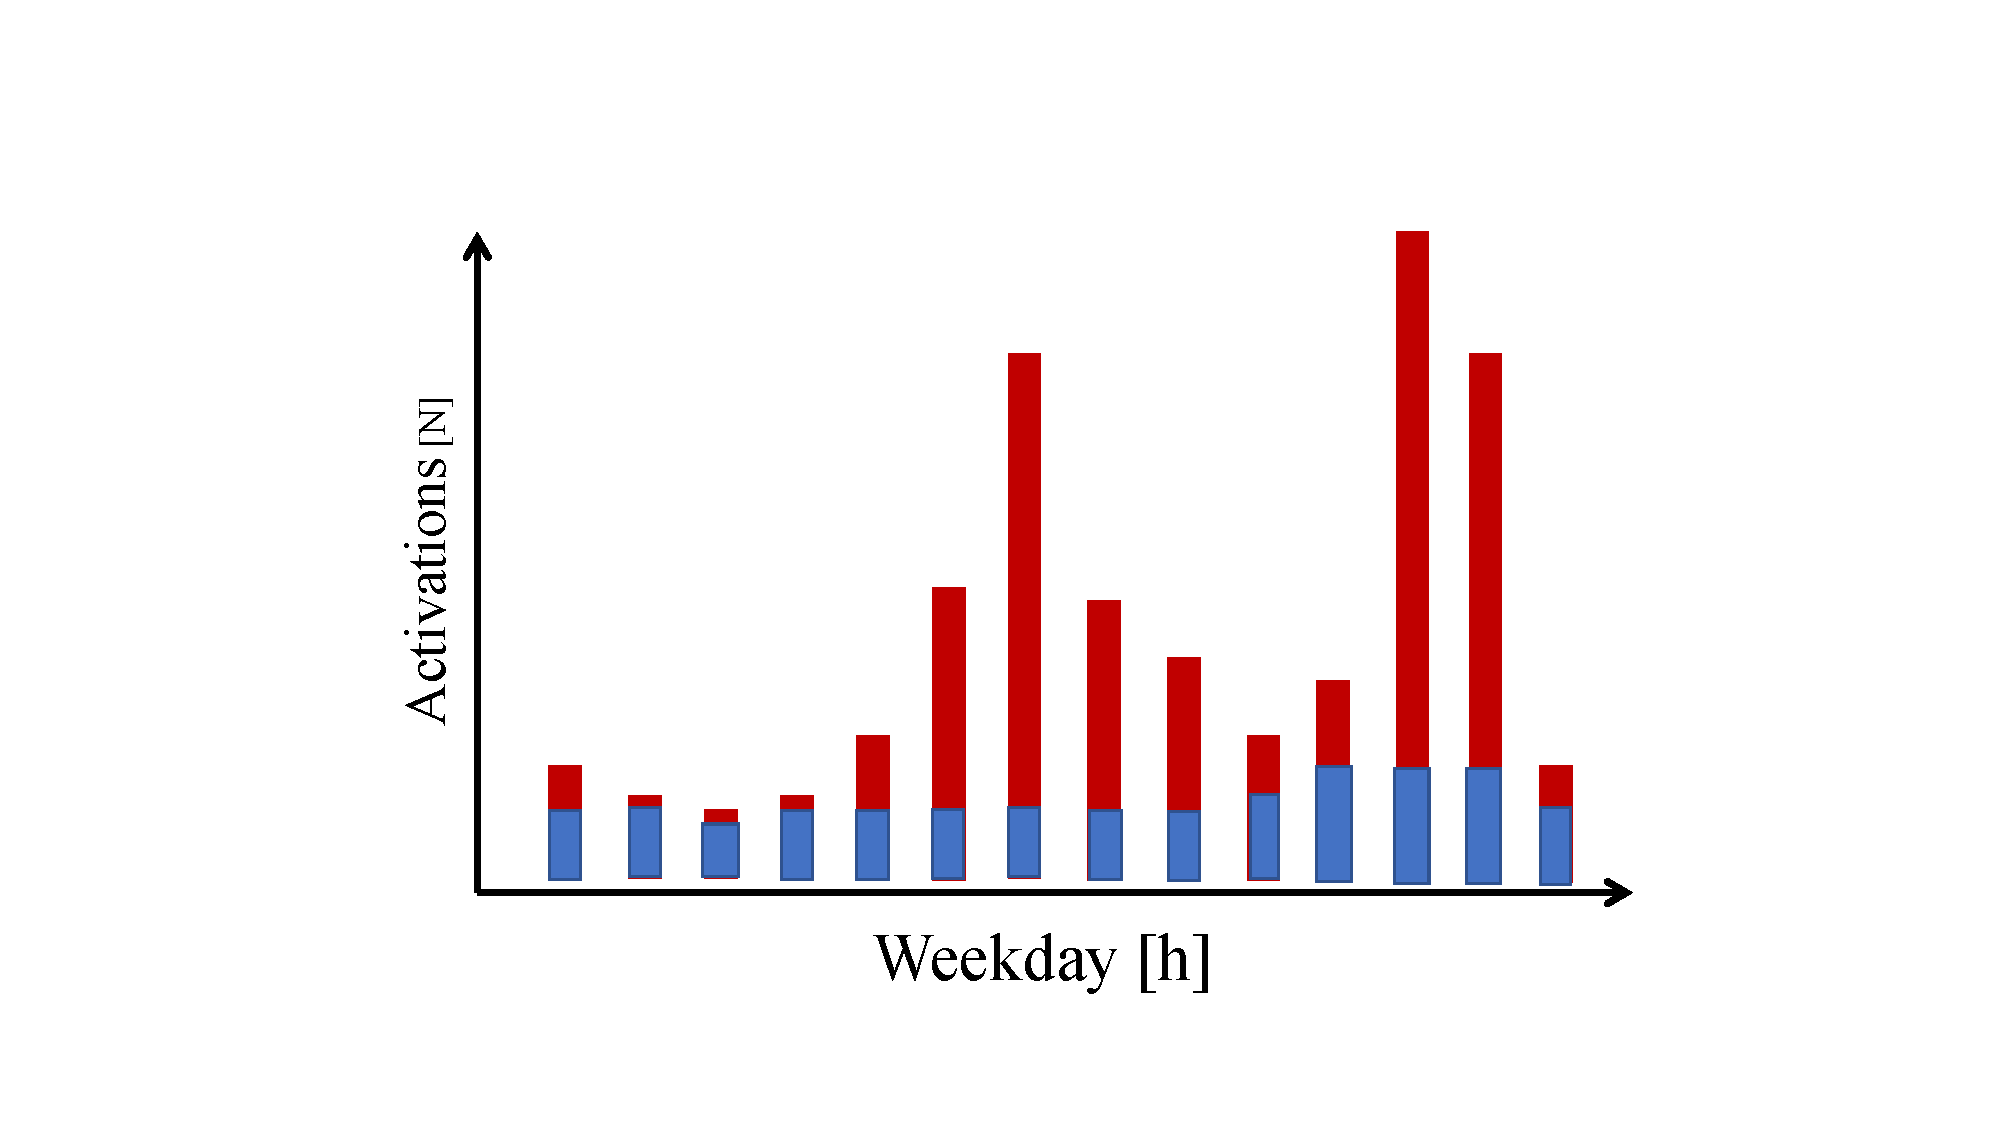
\includegraphics[width=1.2\textwidth]{Figures/profile_sketches/slide8.pdf}
		\label{fig:daily_act_m_profile}
	\end{subfigure}%
	~ 
	\begin{subfigure}{.5\textwidth}
		% \centering
		\caption{Daily per-building per-appliance power LP for appliances A, B and C}
		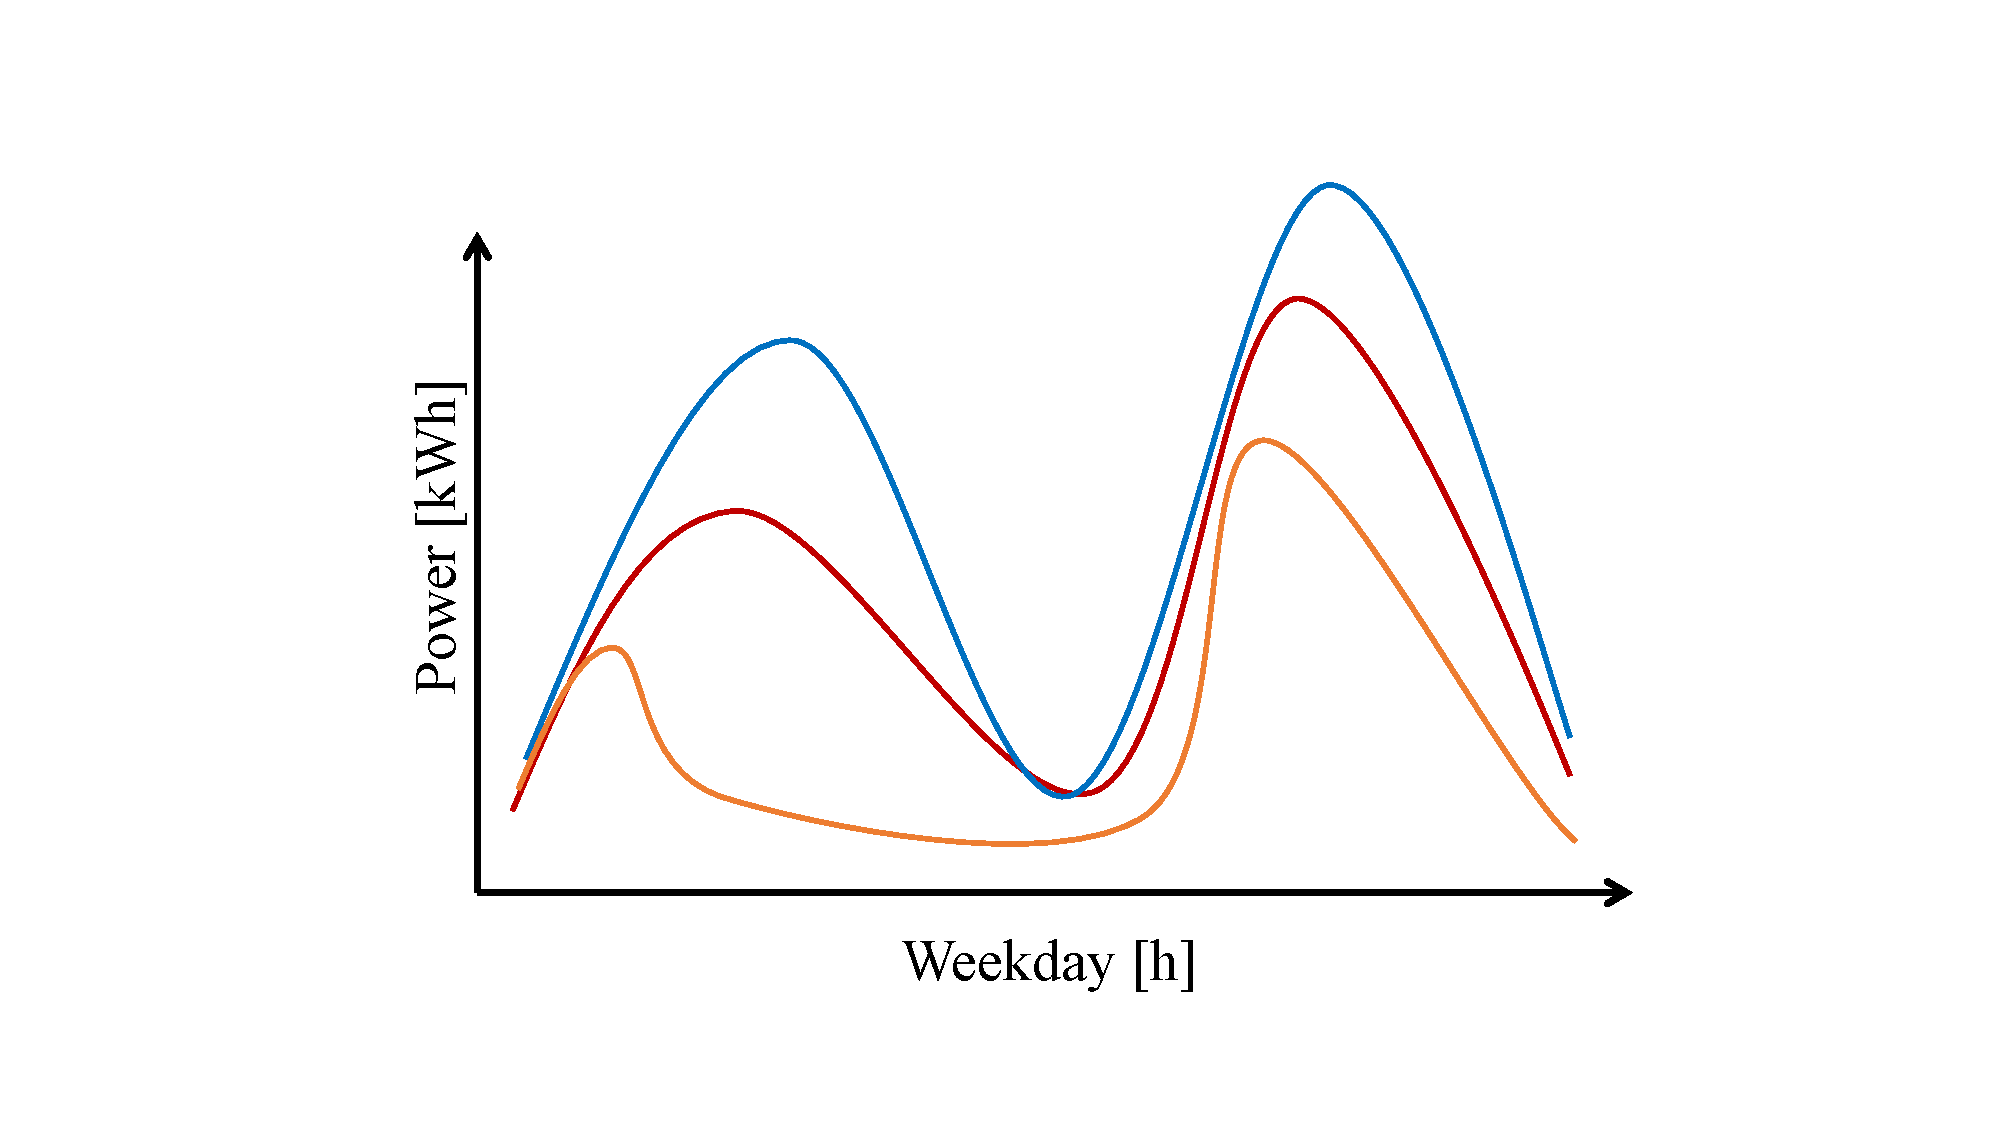
\includegraphics[width=1.2\textwidth]{Figures/profile_sketches/slide2.pdf}
		\label{fig:daily_power_m_profile}
	\end{subfigure}%
	\label{fig:daily_m_profile}
	\caption{Per-building Per-appliance LP}
\end{figure}

\subsubsection{Heatmap LPs}

The last type is a heatmap LP, they can be further divided into two subtypes.
The first type is LPs which consist of two-time dimensions and use color to display consumption.
Such LP can be used to depict both activation and power consumption features and can present per-building consumption as well as per-appliance data.
All this makes them very versatile.
Figure \ref{fig:heatmap_2dtime} provides an example of this subtype.
This format allows us to see the consumption pattern throughout each day in a month.
The brightness represents the activity of the household or a particular appliance.
The brighter the plot, the more activity for that hour of that day of the month.
One thing to keep in mind when reading such a profile is that the origin is placed in the upper left corner.

\begin{figure}[H]
	\centering
	\caption{Number of daily activations/power consumption of one appliance/house in one-month period}
	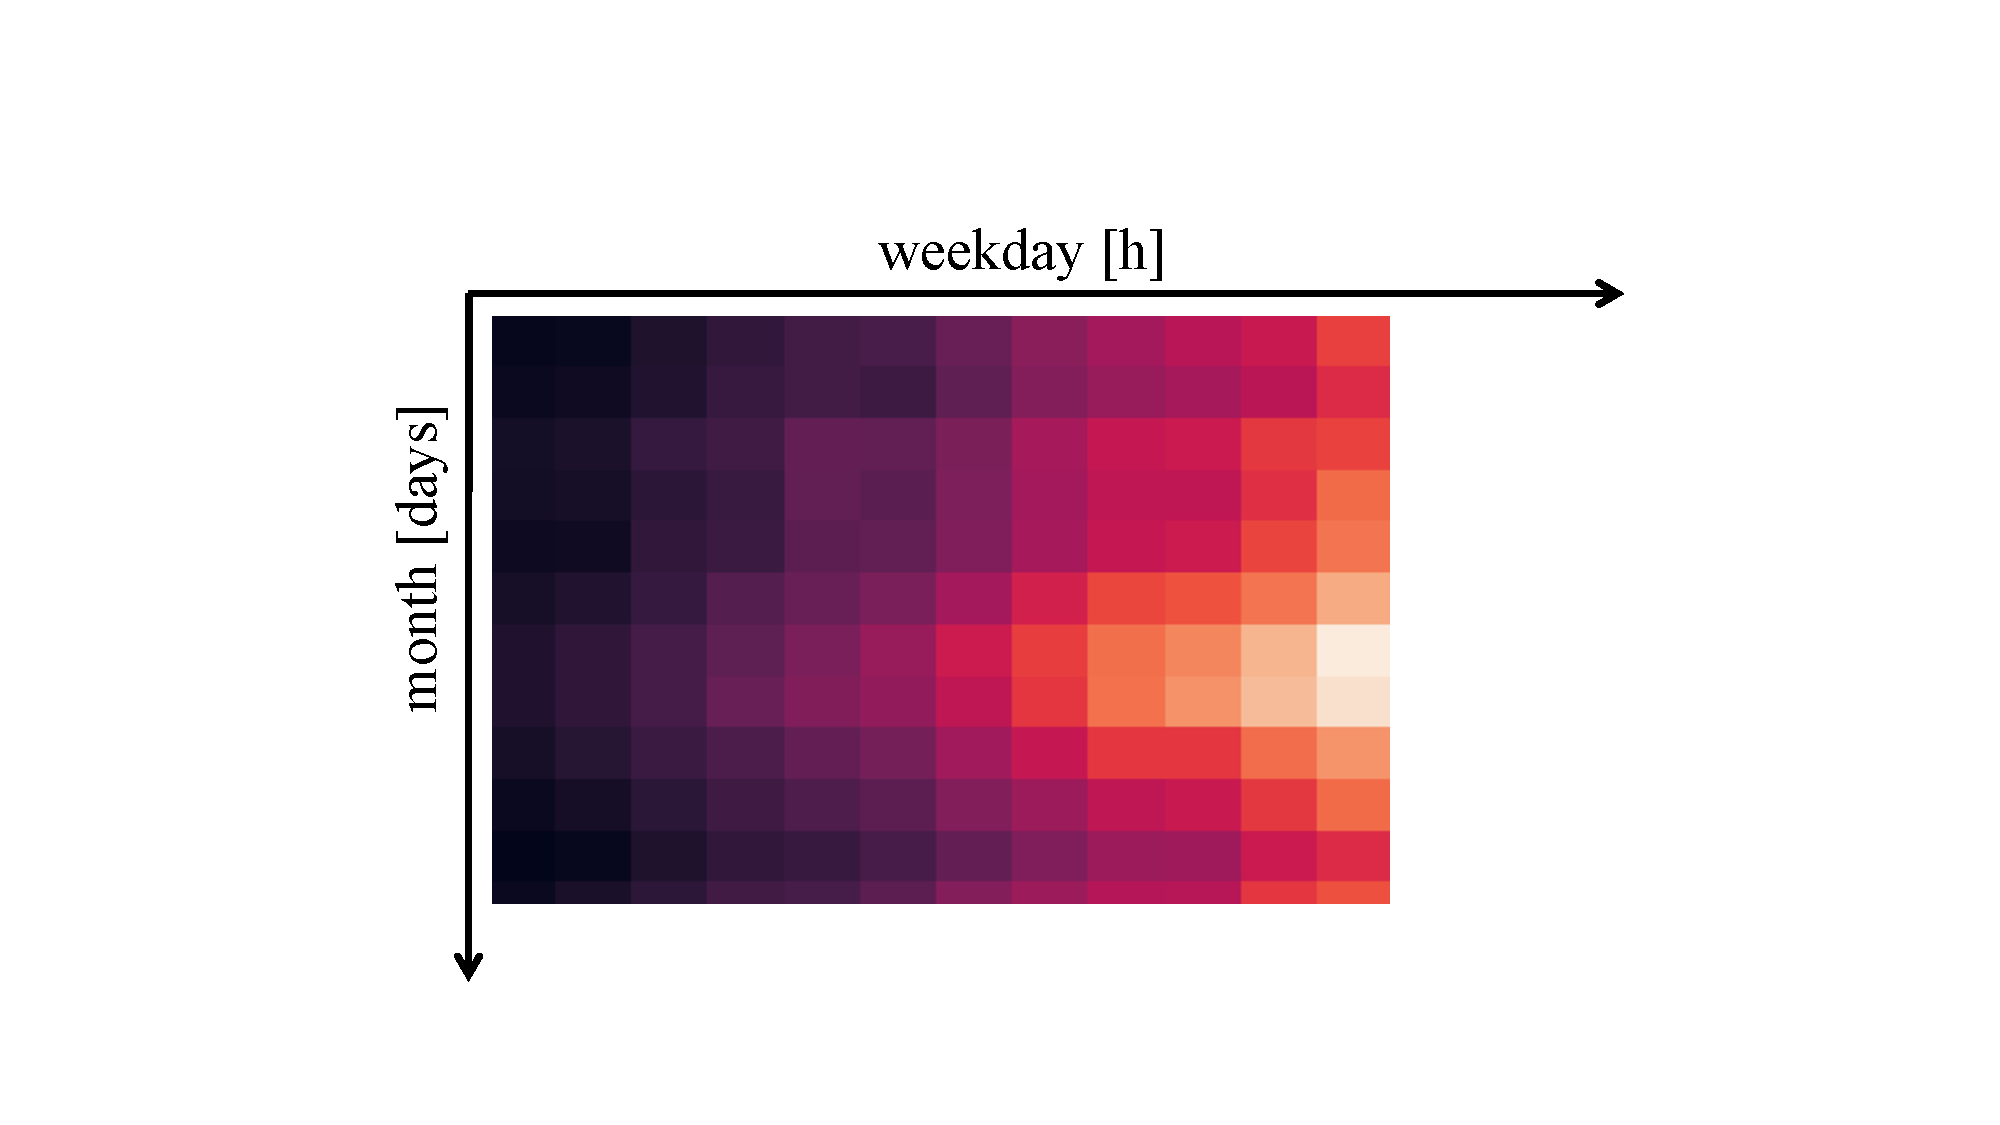
\includegraphics[width=0.9\textwidth]{Figures/profile_sketches/slide10.pdf}
	\label{fig:heatmap_2dtime}
\end{figure}

The second subtype is essentially Per-building Per-appliance LP, just portrayed differently.
Instead of plotting consumption data as the sum of contributions from each appliance, we present their consumption side by side.
These LPs share the same uses as Per-building Per-appliance LPs, given their fundamental similarities.
Figure \ref{fig:heatmap_all_appl} provides a sketched example of this subtype.

\begin{figure}[H]
	\centering
	\caption{Consumption for each appliance in a day}
	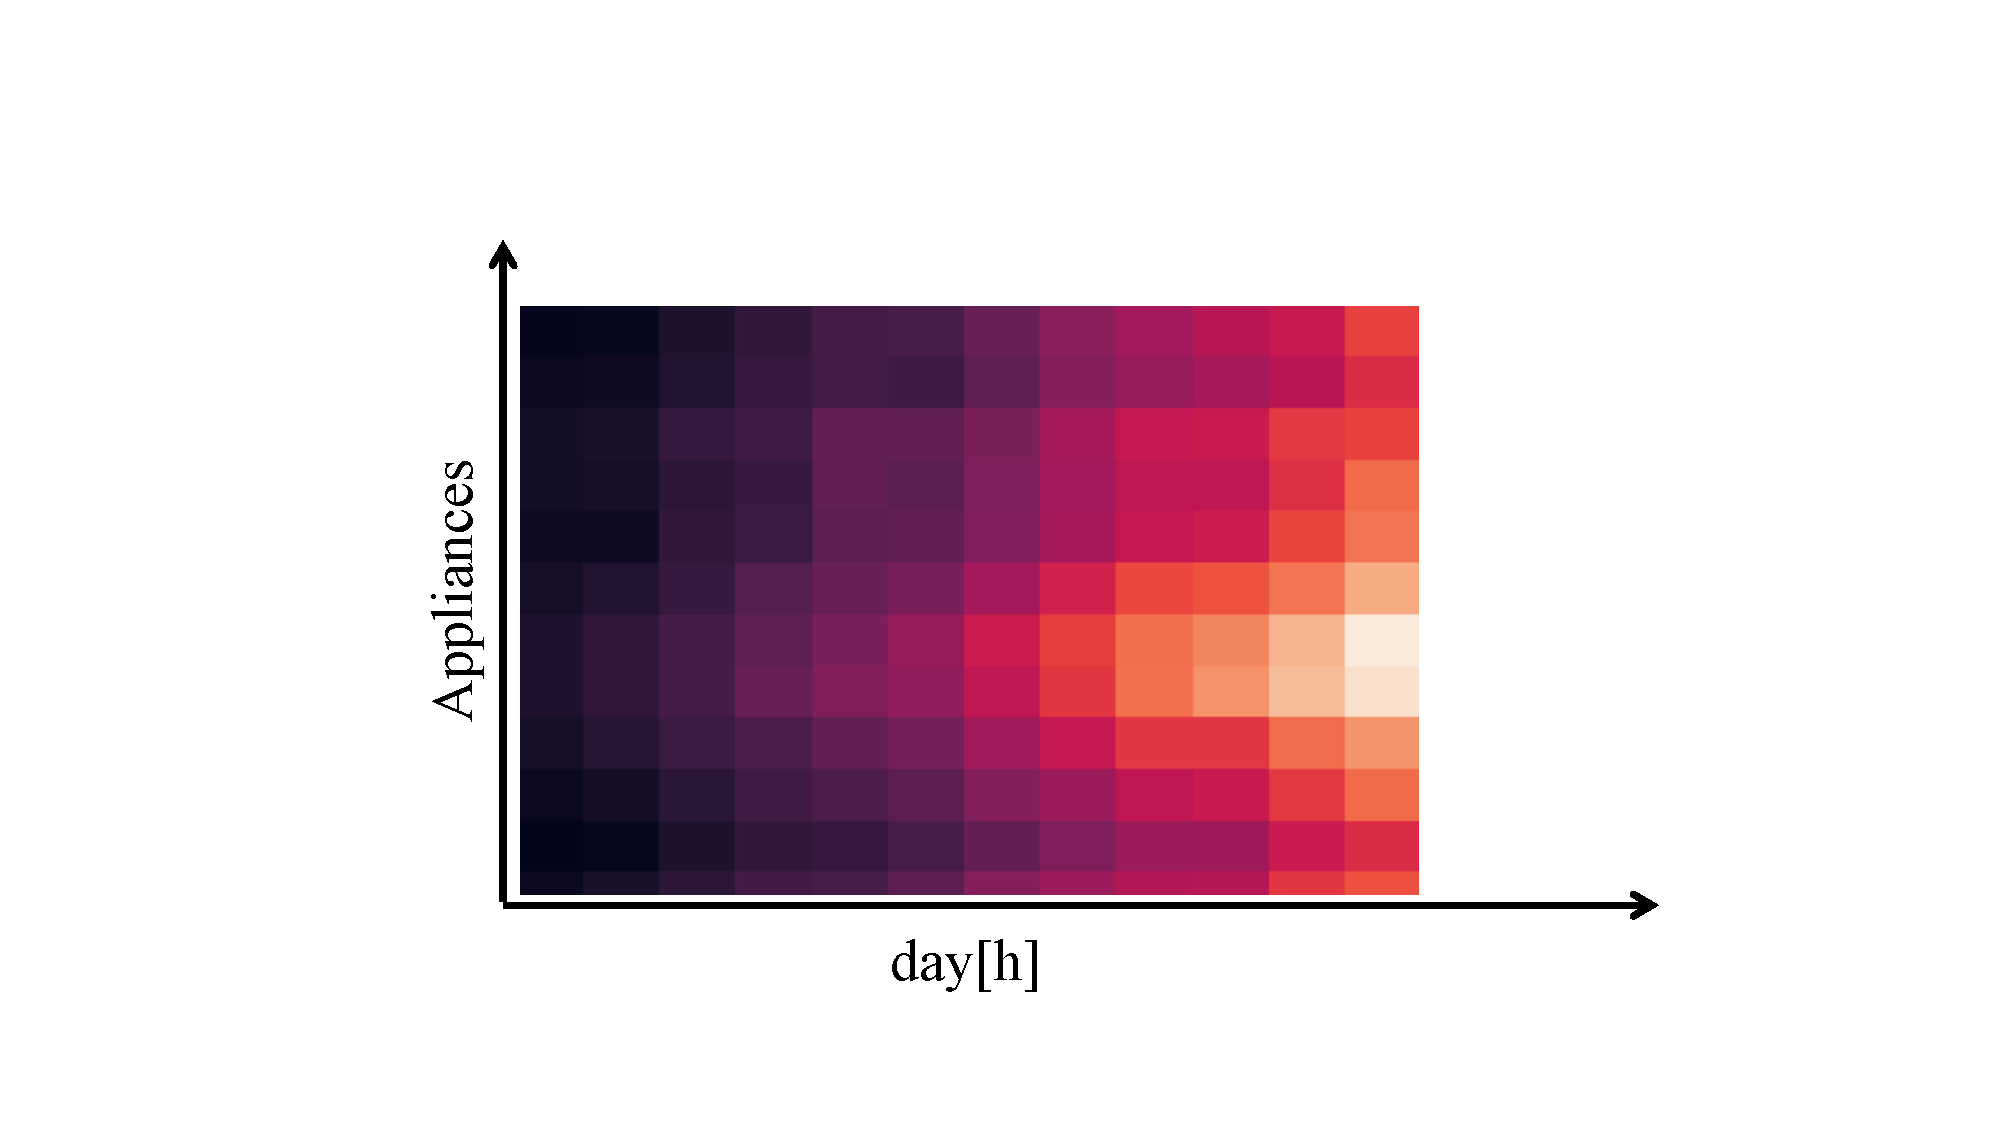
\includegraphics[width=0.9\textwidth]{Figures/profile_sketches/slide12.pdf}
	\label{fig:heatmap_all_appl}
\end{figure}

While there are many features and many more types of LPs out there, we have selected the ones that are most commonly used.
There are also many versions of the LPs above with different timescales, where each has a different use case.
A more comprehensive presentation of these use cases will follow in Chapter \ref{chapter4}, with a detailed classification provided in Section \ref{sec:table_of_profiles}.

\section{LP Use-cases}
\label{sec:use_cases_tree}

\begin{figure}[H]
	\begin{adjustbox}{width=1.0\textwidth,center=\textwidth} 
		% \caption{General classification of LP use-cases}
		\label{tree:clasification_of_use_cases}
		\Tree[.{Use\ Cases} 
		[.Grid\\Managment Energy\\Saving Zero\\Energy\\Buildings Demand\\Response ]
		[.Anomaly\\Detection Elderly\\Care Fault\\Detection ]
		[.Other Product\\Develop-\\ment\\Feedback Occupancy\\Detection Energy\\Stealing ]
		]
	\end{adjustbox}
\end{figure}

The load profiling method has a lot of different use cases across different fields.
In our study, we will categorize these use cases into three classes.

The first class relates to grid management.
For instance, it can be used to save energy by studying users' usage patterns and returning feedback, with suggestions on how to optimize consumption.
In scenarios where buildings have grid batteries and PV installed, the same feedback could be used to minimize the amount of energy being drawn from the grid.
These are so-called zero-energy buildings (ZEB).
Electrical energy providers could leverage demand response programs in combination with the LPs to optimize the management of the grid, with minimal impact on users' daily routines.

The second class involves anomaly detection.
The LPs could be used to help the elderly in case of an accident or even help prevent one. 
They could be used to detect all kinds of early malfunctions in the operation of appliances, which would reduce service costs and save energy.

The final class, labeled 'other', encompasses occupancy detection, development feedback, and energy theft detection as potential use cases where LPs could be applied.

A more detailed description of each use-case with publications will be addressed in the following chapter, specifically in Section \ref{sec:use-cases}.

\section{Data}
\label{sec:data}

To construct the LP, we need time-series data that contains information about energy consumption.
While LPs are generally used to analyze the usage of electrical energy they could be applied in many areas.
For example, LPs could be used to analyze any other utilities such as gas, oil or even tap water. 
Furthermore, while this thesis focuses on analyzing the consumption of electrical energy, LPs can be applied to analyze production.
Finally, while we focused on optimizing residential energy consumption patterns, the same approach can be applied extended to industrial or office settings.

In the thesis, we used the following five datasets:
 UK-DALE \cite{UKDALE}, REFIT \cite{REFIT}, ECO \cite{ECO}, REDD \cite{REDD}, and iAWE \cite{iAWE}.
All datasets measured electrical energy consumption in residential buildings.
They include main smart meter data, as well as sub-meter data for each appliance in a dwelling. 
While some datasets offered versions with high frequency with sampling rates up to 40 kHz,
we focused on the low-frequency variations with sampling rates at around 1 Hz.

The utilized datasets had frequencies ranging from 1 Hz for the ECO dataset, down to 1/8 Hz for the REFIT dataset.
To ensure compatibility, we resampled all datasets to 1/6 Hz.
The missing samples were forward-filled with a limit of 5, meaning that if up to 30 s of data was missing, its value was set to the last known value; otherwise, it was left missing.
For easier management, datasets will be divided into 1-hour intervals.
The exact methodology will be presented in Chapter \ref{chapter3} of the methodology section.

\section{Contributions}
\label{sec:contributions} 

The primary objective of the master's thesis is to propose suitable LPs for supporting residential building consumption optimization and elderly care management.
To achieve this goal, we propose the following steps, where each step is a contribution to the scientific community.

\begin{enumerate}
	\item[1.] Surveying the state-of-the-art LPs (Chapter \ref{chapter2})
\end{enumerate}

The first contribution involves a review of existing research and use cases.
Drawing from various publications, we construct a comprehensive table of LPs. 
We are the first to analyze LPs from this perspective, which provides an overview of related work by mapping it onto a table.
This table reveals LPs that have not yet been utilized.
We then examine use cases to determine the potential application fields for each LP.

\begin{enumerate}
	\item[2.] Development of multidimensional activation LPs (Chapter \ref{chapter4})
\end{enumerate}

Empty gaps in research motivated us to pursue our next contribution: the development of multidimensional activation LPs. 
Here we offer an in-depth look into both existing and newly proposed LPs, showcasing how they represent consumption patterns.
We also apply these LPs and discuss potential scenarios and use cases for their application. 
Each LP reveals a different pattern and, therefore, serves a different use case. 

\begin{enumerate}
	\item[3.] Visual analysis of activation LP's (Chapter \ref{chapter5})
\end{enumerate}

The third contribution involves exploratory data analysis (EDA) through visualizations.
Here, we leverage the LPs that we have proposed and analyzed, using the t-SNE dimensionality reduction algorithm to understand the relationships within the data.

\begin{enumerate}
	\item[4.] Propose a new anomaly detection method for elderly care (Chapter \ref{chapter6})
\end{enumerate}

This newly obtained knowledge should help us provide the final contribution, where we utilize LPs that have not been previously considered.
We design and construct an assisted living system for elderly care by utilizing one of the proposed LPs.
The system can detect anomalies in the daily routine of an elderly individual.
Should an anomaly is detected, the caregiver is notified to check on the individual. 
This system is simple, efficient, and ready for real-world application.
\label{chapter2}
\chapter{Definitions}

Author \cite{Review2021} defines terms as following

\begin{itemize}
	\item Residential: private residences, with no commercial usage, occupied by one or more persons either full-time or part-time during a calendar year.
	\item Load: the electricity that all the electricity-powered devices in the household consume in unit time.
	\item Profile: a graph representing the significant features of the electricity load over time.
	\item Model: "a formal system that represents the combined processes" \cite{KAVOUSIAN2013184} of electricity consumption by all the electricity-powered devices in a private residence/number of residences.
\end{itemize}

Commonly load profile is a term defined as aggregated power usage of all appliances in a house. 
Sometimes load profile is used to describe appliance-level load profiles. 

The load profile is most commonly presented with a curve, that shows daily power usage.

\begin{figure}[H]
	\centering
	\caption{"Clustered load profiles. The graph was published by \protect\cite{GERBEC2005}"}
	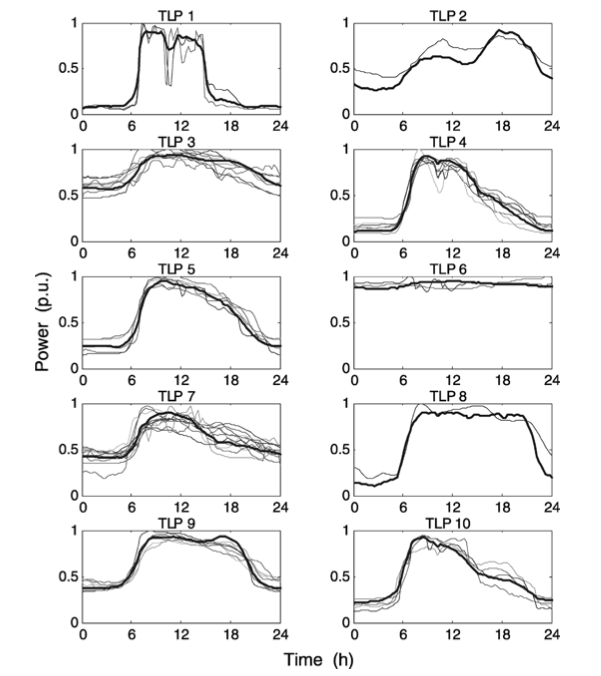
\includegraphics[width=0.9\textwidth]{Figures/clustered_profiles.png}
	\label{fig:profiles}
\end{figure}

Figure \ref{fig:profiles} depicts 10 clusters of daily load profiles. 
This is not the only way to present it, for example, author \cite{Park2019} used an image-based presentation.


% Chapter Template

\chapter{Methodology} % Main chapter title
\label{chapter3} 

The following chapter includes methodological procedures that are common for all chapters.
More detailed methodological procedures will be described in each chapter separately. 

\section{Data}

We already briefly presented the datasets in the first chapter in section \ref{sec:data}.
Here, we will do an in-depth presentation of the datasets and present how we processed and cleaned the data. 

\subsection{Dataset selection}

The Table \ref{tab:other_datasets} was published on the NILMTK \cite{nilmtk} wiki page. 
NILMTK is a tool developed by authors in paper \cite{nilmtk}.
It intends to make the development of NILM algorithms easier by standardizing a format in which building energy consumption datasets are stored. 
They also developed converters to convert existing datasets into a universal format.
This enables engineers to simply load and process multiple datasets.
NILMTK includes a dataset converter from most of the datasets from table \ref{tab:other_datasets}.
\begin{table}[H]
    \centering
    \caption{Pruned version of the Table published by authors on NILMTK\protect{\cite{nilmtk}} wiki page. Full table available here \protect{\url{https://web.archive.org/web/20190607094329/http://wiki.nilm.eu/datasets.html}}.}
    \resizebox{\textwidth}{!}{\begin{tabular}{|l|l|l|l|l|l|l|l|l|}
    \hline
        \textbf{Dataset} & \textbf{Sampling rate} & \textbf{Duration } & \textbf{ Buildings } & \textbf{Subject} & \textbf{Country} & \textbf{Availability} \\ \hline
        Dataport & 1 Hz to 1 minute & 4+ years & 1200 & multiple & US & Licensed \\ \hline
        BLOND-50  & 50 kHz/6.4kHz & 213 days & 1 & office & Germany & Public \\ \hline
        FIRED & 12 kHz to 1 Hz & 101 days & 1 & residential & Germany & Public \\ \hline
        REDD & 16500 Hz / 1 Hz & 100 days & 5 & Residential & US & Request access \\ \hline
        BLUED & 12000 Hz & 7 days & 1 & Residential & US & Request access \\ \hline
        UK-DALE & 16000 Hz / 1 Hz & 2 years & 6 & Residential & UK & Public \\ \hline
        PLAID & 30000 Hz & 5 seconds & 55 & Appliances & US & Public \\ \hline
        WHITED & 44000 Hz & 5 seconds & 9 & Appliances & Multiple & Public \\ \hline
        Tracebase & 1 Hz & 1 day & 158 & Appliances & Germany & Request access \\ \hline
        DRED & 1 Hz / 1 min & 150 days & 1 & Residential & Netherlands & Public \\ \hline
        AMPds & 1 minute & 2 years & 1 & Residential & Canada & Public \\ \hline
        RAE & 1 Hz & 72 days & 1 & Residential & Canada & Public \\ \hline
        iAWE & 1 Hz & 73 days & 1 & Residential & India & Public \\ \hline
        HES & 2 minutes & 1 year & 251 & Residential & UK & Request access \\ \hline
        REFIT & 8 seconds & 2 years & 20 & Residential & UK & Public \\ \hline
        ECO & 1 second & 200 days & 6 & Residential & Switzerland & Public \\ \hline
        COMBED & 30 seconds & 30 days & ~ & Office & India & ~ \\ \hline
        IHEPCDS & 1 minute & 4 years & 1 & ~ & France & ~ \\ \hline
        SMART & 1 Hz & 60 days & 3 & ~ & USA & ~ \\ \hline
        LIT-Dataset & 15 kHz & 30 seconds & 26 & Residential & Brazil & Public \\ \hline
    \end{tabular}}
    \label{tab:other_datasets}
\end{table}

The reason why more datasets were not selected from the Table \ref{tab:other_datasets},
was because we followed the criteria:
\begin{enumerate}
    \item Sampling rate between 1 Hz and 1/10 Hz
    \item Duration more than 30 days
    \item Subject had to be a residential area building
    \item Include main meter as well as sub-meter measurements
    \item Has to be accessible
\end{enumerate}

After applying these criteria we were left with the following datasets:

\begin{itemize}
    \item UK-DALE \cite{UKDALE}
    \item REFIT \cite{REFIT}
    \item ECO \cite{ECO}
    \item REDD \cite{REDD}
    \item iAWE \cite{iAWE}.
\end{itemize}

\subsection{Processing}
After datasets were obtained and converted they were ready to be processed.
We decided to slice the data into hourly slices so that it will be easier to find missing data and build LPs.

Firstly we resampled the time series data  1/6 Hz. 
This had to be done since datasets were sampled at different frequencies.
A frequency of 1/6 Hz is commonly used since it has a good ratio between resource usage and NILM algorithm performance.
Resampling was done using Pandas resample. 
We used a forward fill parameter with a limit of 5.
This means that in case of missing data, we will fill in no more than 5 samples, with the last known value.
Secondly, we sliced the time series data into hourly slices. 
With one sample every 6 seconds, there were roughly 60 samples in every slice.
Thirdly, we removed slices with missing data.
This was done for all slices where there was more than 20 \% of data missing.
In cases where less than 20 \% of data was missing, we forward-filled it with the last known value.
In the worst case, we forward filled 12 samples. 
Finally, resampled and cleaned data was stored in the following manner.
\begin{verbatim}
   /dataset/appliance/building/
\end{verbatim}

\subsection{Training and health}

\subsection{Datasets and evaluation} \label{ssec:ds_eval}

The data was split into train and test sets, where 80 \% of the data was used for training and 20 \% percent of the data for testing.
The data was split based on the number of samples, so in some cases where there is a lot of missing data, the time window of test data might be longer, although it contains only 20 \% of the samples.

\subsubsection{REFIT}
The REFIT \cite{REFIT} dataset included data for more than 15 buildings, as can be seen in the Figure below.
The dataset in general is of the highest quality since it is the longest with the least missing data.
This means this dataset should give the most relevant results.
\begin{figure}[H]
	\centering
	\caption{Timeline for REFIT}
	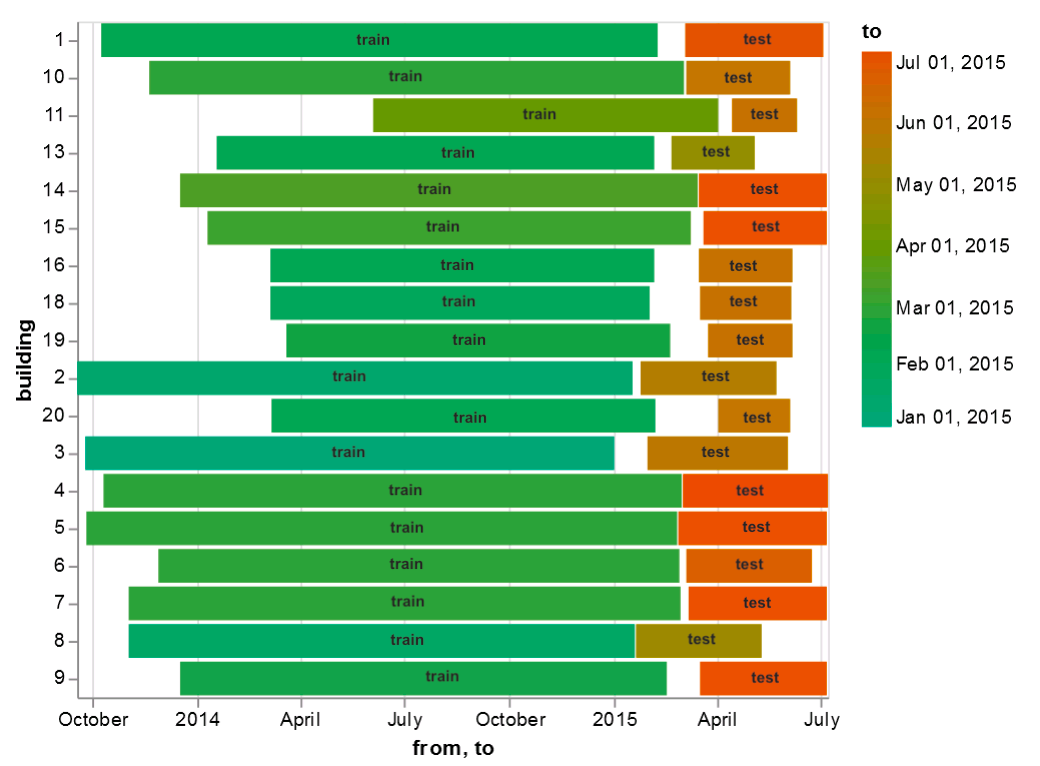
\includegraphics[width=1\textwidth]{Figures/EC/refit_timeline.png}
	\label{fig:refit_timeline}
\end{figure}

\subsubsection{UK-DALE} 

Through the UK-DALE \cite{UKDALE} dataset is of similar size, most of the data is from building 1.
In general, it includes 5 years of data, but only for some appliances, where many appliances are rarely used.
When taking all of this into account, there were too many issues with building 1, and it was simply ignored.
Another issue that can be seen in Figure \ref{fig:ukdale_timeline} is that there is not enough data for 
building 3. The test includes only a week of data, which is not enough for representative results, therefore it was ignored.
The rest of the buildings seem healthy.

\begin{figure}[H]
	\centering
	\caption{Timeline for UK-DALE}
	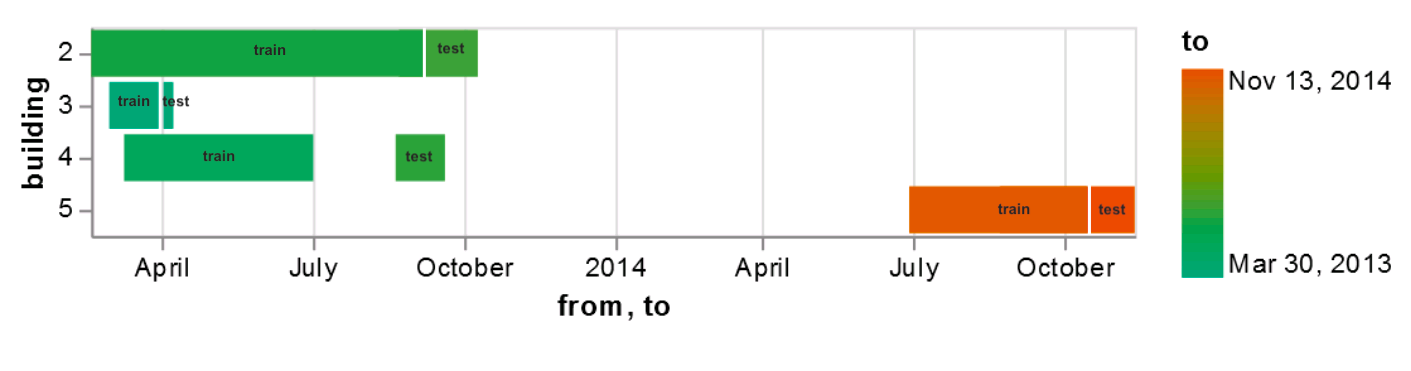
\includegraphics[width=1\textwidth]{Figures/EC/ukdale_timeline.png}
	\label{fig:ukdale_timeline}
\end{figure}

\subsubsection{ECO}
ECO \cite{ECO} dataset has a length of data similar to UK-DALE. 
The only issue is building 1, where there is a lot of missing data.
This is a good example of how data is split, it is split based on several samples,
meaning that there is 80 \% in the train bar, due to missing data the second bar is longer. 

\begin{figure}[H]
	\centering
	\caption{Timeline for ECO}
	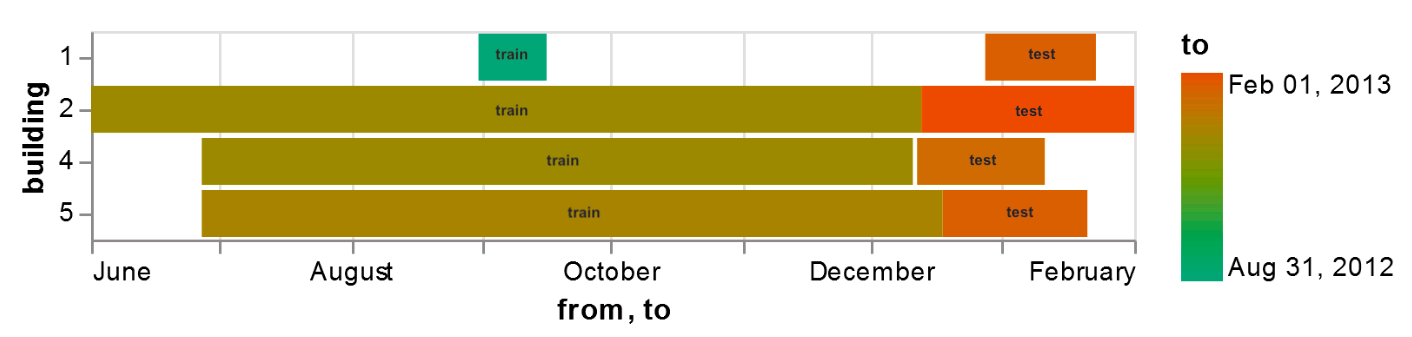
\includegraphics[width=1\textwidth]{Figures/EC/eco_timeline.png}
	\label{fig:eco_timeline}
\end{figure}


\section{Tools Used}



To process the data and to obtain the results the environment and virtual machines from Google Colab \cite{colab} were used.
They offer access to Google GPU-accelerated compute machines with 12 GB of RAM. 
Colab also offers access to Drive cloud storage, where the dataset and results were stored.
While running the experiments, we made use of Drives 100 TB pooled cloud storage, which is available to students of the University of Ljubljana. 
For development and version control, GitHub was used. 

Within the Colab which uses a Jupyter \cite{jupyter} environment at its core, various python libraries were used.
To store and read the datasets in hdf5 format we used h5py  \cite{hdf5} and Pickle  \cite{pickle}.
To load datasets into RAM and then handle them, the pandas  \cite{pandas} library was used.
For handling the large matrices and calculating we used NumPy  \cite{numpy}.
To present the data with graphs we have used Matplotlib  \cite{matplotlib} and to present data with heatmap Seaborn  \cite{seaborn}.
For easier implementation, such as of the t-SNE, a Scikit  \cite{scikit} and SciPy  \cite{scipy} libraries were used.


\label{chapter4}
\chapter{Possible use cases}

The load profiling method has a lot of different use cases across different fields.
In our case, we will split use cases into three classes.

The first class is grid management.
For example, it can be used to save energy by studying users' usage patterns and returning feedback.
Electrical energy providers could use that same data to optimize the management of their grid, with minimal impact on users' daily lives.

The second class is anomaly detection.
The load profiles could be used to help the elderly in case of an accident and help prevent one. 
They could be used to detect all kinds of early malfunctions in the operation of appliances and help save energy.

The last class is miscellaneous or other where occupancy detection, research, and development are all areas where profiling could be used. 

\section{Grid management}

\subsection{Zero energy buildings and energy saving}

As mentioned before many applications for load profiling could be used to reduce energy use and increase energy efficiency. 
With the emerging EV-market and ever-increasing installation of heat pumps, more and more energy is being used in form of electricity. 
This means, that most of the current power grids would have to be upgraded to keep up with demand.

On the other side, more and more photovoltaic systems are being installed,
which is slowly shifting energy production towards end-users.
Slowly energy grid is starting to shift towards so-called distributed energy resources or "DER" \cite{MORENOJARAMILLO2021445}.
DERs include all kinds of micro-energy sources such as PV, wind power, water power, and all kinds of energy accumulators that can store 
and release energy when needed such as heat pumps with hot water storage, home batteries, and EVs that can be used as a battery.

With smart management, these appliances could be used in a way that would reduce the net flow of energy and alleviate the load off the power grid.
A way to achieve this is via load profiling and load modeling. 
To manage the appliances, a control system would have to be put in place \cite{DirectLoadControll2021}.
It would be enough to control a few appliances that consume most of the energy. 

Since consumers take part in producing the energy, they are often called "prosumers" \cite{Prosumer2016}.
They will be an essential part of the European Union's plan to reach zero-energy buildings
and near-zero-energy buildings \cite{eu2021}. The directive was accepted in 2010 and was recast in 2021.
The plan is set to be realized in the next decade.

An actual use case would be an EV owner with an installed PV system and heat pump, who works from home on occasions.
In this case, two profiles would be developed. Normal workday and work from home day.
Additional information would be obtained from the users calendar. 
On a normal workday, the system would use PV energy to heat the water and store it, based on the user profile.
On work-from-home days, the system would start charging the car with the morning sun, using only the PV energy. 
In the evening hours, when consumption rises and production falls, EV could inject the power back into the house. 
Again using appliance load profiles to mitigate net energy flow as close to zero as possible (zero-energy building).
With the ever-increasing power capacity and increasing range of EVs, more and more battery capacity could be used for mitigation. 
In the case of grid batteries, similar steps could be taken.
This process is called vehicle-to-grid, and it is an important step towards zero-energy buildings \cite{EV2018} and \cite{EV2020}.

One other way to use user load profiles is to optimally distribute the load by studying users usage patterns as \cite{Chuan2014} and \cite{shift2015} proposed in their papers. 
This could be further extended to neighborhoods connected into peer 2 peer energy distribution networks.
As mentioned earlier, the way to save energy consumption is to distribute it as locally as possible. 
Knowing usage patterns of all peers, the system could optimally distribute the energy using DERs across all homes without dwellers even noticing.

Another use case could be using a heat pump and heat storage,
where besides users usage patterns system would also obtain weather forecasts from the internet.
Heat pumps that extract heat from the air are more efficient when temperature differences are smaller. 
The heat pump could store energy when warm and release the energy when cold.
Based on the user usage profile, energy could be optimally distributed.

Many papers have been published, where authors explored ways to reduce the energy consumption of users by studying user consumption patterns,
such as \cite{energy_saving3}, \cite{energy_saving1}, \cite{energy_saving4} and \cite{energy_saving3}.
Energy saving is done through instant feedback, reduction goals, rewards, and by comparing their user profile to the average user as the authors did in \cite{Csoknyai2019}.
Source \cite{eu2006} states that as much as 20 \% of energy could be saved by managing the consumption.

\subsection{Demand response}

An increasing percentage of renewable resources is troubling energy distributors, due to the nature of renewable resources.
In the prior chapter, it was mentioned how energy-saving measures would benefit users and their peers.
One other use case would be cooperation between end-user and energy distribution companies.
Joint actions between them would benefit both as authors show in \cite{cooperation2008} and \cite{cooperation2010}

The electricity provider could control the main appliances so that load on the power grid is uniform,
with as few peaks and valleys as possible. For this to function, users would have to allow the installation of energy meters and controllers 
on appliances that use the most electricity \cite{gridDirectControll2015}. One way to achieve this is to control the voltage of loads \cite{controll2014} the other
way is to shift the loads in time \cite{shift2015}.
This process is called direct load control \cite{DirectLoadControll2021}, and it is part of demand response program \cite{DemandResponse2018}.

"DR program is a voluntary PJM program that compensates end-use (retail) customers for reducing their electricity use (load)
when requested by PJM during periods of high power prices, or when the reliability of the grid is threatened." \cite{DemandResponse2018}

The benefit to the user would be lower the cost of charging EVs and heating the building.
This is already done through so-called small and high tariffs.
More detailed user load profiles would enable the electricity provider to introduce real-time tariffs to the user.

The user would have three options. The first one would be that users can use the appliances as freely as they desire, this would result in a normal tariff.
The second option would be to use the appliances as regularly as possible, this would lead to lower tariffs.
The third option would be to leave the management of main appliances to the electricity provider.
The provider would combine the user appliance load profile and the real-time market price of energy to optimize the cost \cite{optimiseCostShift2015}.
This would lead to free or even negative prices of electricity since distribution companies have to keep the frequency of the grid as stable as possible.

For them to stabilize the frequency, they sometimes have to resort to load shedding.
Load shedding is a process where a load is disconnected from the grid to keep the grid in sync \cite{loadShedding2006}.
Commonly whole neighborhoods are being disconnected, affecting their daily lives.
Using user load profiles, distribution companies could disconnect the load in a way that would minimally affect the end-user. 
When they would need to load the grid due to low demand, they could charge EVs free of charge or even pay to do so. 
This benefits the company as well since they do not need to lower energy production, which can be expensive. 

\section{Anomaly detection}

One use case of anomaly detection was already mentioned in the Elderly care chapter.
One more thing that could be detected, using load profiling, would be the altered operation of appliances.
In the case of a fridge, the system would detect that duty cycles are too long.
The increased duty cycle can be caused by cooling liquid leakage, fridge being open or compressor motor malfunction.
Heat pumps work on the same basis as fridges, meaning the same anomalies could be detected. 
The malfunction could also be detected in heating element appliances such as toasters or boilers. 
Since mentioned appliances are one of the largest consumers in a household,
early enough detection could lead to large energy-saving benefits \cite{NILMAD2019}.

\subsection{Elderly care}

Demographic changes i.e. aging population is an increasing socioeconomic issue.
The elderly are facing many issues when staying at home alone for extended periods.
Accidents such as falls or the inability to do choirs due to health-related issues or even dementia-induced issues 
such as leaving appliances on for long periods could all be detected, using sub-meter data such as authors \cite{elder1} and \cite{elder2}
explore in their papers.

To detect falls or other issues a normal daily appliance use profile would be developed.
It would involve routine behavior of users such as turning on the coffee machine in the morning, the stove and oven at the noon or using the toaster in the evening.
All these routines could be measured and tracked. Using this data, a profile would be developed.
The probability of an anomaly and a threshold would enable the system to detect an issue.

An example would be: the coffee machine not turning on in the morning or the stove and kitchen vent not being used at the noon.
Another issue could be detected if the appliance would be used more frequently or for extended periods of time. 
This could indicate that the user forgot to turn off the stove, oven, or even a light. The same system could detect 
that a fridge or a freezer was left open since the duty cycles would be longer and more frequent. 
As soon as the issue would be detected it would notify the caregiver to check on the patient.

\section{Other}

Load profiling could also be used as feedback for the engineers and designers,
of how a certain device is being used and if it is being used as designed. 
This would enable the manufacturers to improve their products according to 
user's needs, without unnecessary features.

\cite{energyStealing2018} uses anomaly detection algorithms and load profiling to detect energy lost due to non-technical losses.
This occurs after the smart-meter is exposed to cyber or mechanical attacks and its measurements are off. 

One other use case could be occupancy detection of buildings such as the authors explore in \cite{occupancy2013}. Information about 
occupancy could be used as part of elderly care monitoring or in the case of building
automation, to run certain tasks when a user enters or leaves the room or a building.
\chapter{Exploratory data analysis of LPs using t-SNE} 

\label{chapter5} 

\section{Introduction}

LPs can be used to understand the consumption patterns of appliances or buildings.
The one thing they do not offer is a comparison between activation patterns.
To achieve this we can utilize various dimensionality reduction algorithms. 
In the process of dimensionality reduction, these algorithms map similar LPs closer together compared to dissimilar LPs.
This enables us to have an insight into similar activation patterns across various entities.
It enables us to visualize and compare LPs of buildings and appliances, to find the differences and similarities in their activation patterns.

In this chapter, we will explore the use of t-distributed stochastic neighbor embedding (t-SNE) for Exploratory Data Analysis (EDA) on LPs.
The t-SNE is a non-linear dimensionality reduction algorithm, used to visualize high dimensional data in usually two or three dimensions.
We will delve into the details of what t-SNE is and how can it be applied to the LPs.

To achieve this goal, we will first provide a brief overview of t-SNE and its application to LPs.
Next, we will describe our methodology for using t-SNE to analyze LPs and compare activation patterns.
Finally, we will present the results of our analysis and discuss their implications for understanding energy consumption patterns.

The clustering of similar LPs was researched many times before, as it was described in related work Chapter \ref{chapter2}.
We will be working with dimensionality reduction, where clusters are usually formed as a side product.
The following clustering publications are worth mentioning.
We have seen that authors \cite{GERBEC2005}, \cite{Jeong2021} and \cite{Joana2012} have clustered regular one-dimensional LPs, as well as with 2D image-based load profiling in publications published by authors \cite{Park2019}. 

The publication by authors \cite{sne_energ} compared various dimensionality reduction techniques for clustering and visualization of LPs.
Their goal was to compare Principal Component Analysis, Isometric Feature Mapping, Sammon Mapping, Locally Linear Embedding and Stochastic Neighbor Embedding.
They used daily power LPs from residential and industrial areas.
This publication was of the closest resemblance to our goals, that we were able to find. 

In all cases, work has been done with the power LP, whereas in this case, we will try to find similarities between activation profiles using a t-SNE algorithm.
Most of the publications used single-time dimensions, whereas we will use two-time dimensions.

Although the use-cases were presented in-depth in Chapter \ref{chapter2}, it is worth mentioning one specific use case.
The increasing price of energy resources, could lead to over-saving and living in cool homes.
By using similarity metrics between profiles across different buildings, it would be possible to detect outliers when it comes to heating. 
With this approach, it would be possible to detect users, that are living in below-average cool homes and offer them cheaper plans. 

\section{Methodology}

\subsection{LPs}

\subsubsection{Weekly-Daily LP}

During testing, a weekly-daily LP constructed from a month of data will be used.
Y-axis will present the days in a week and X-axis presents the hours in a day.
Weekdays are labeled from 0 to 6, and hours from 0 to 23.
Since we are working with images, the origin is placed in the upper-left corner. 
This means that a pixel in the upper-left corner presents the first hour of a week,
this would be a Monday from midnight to one o'clock. 
The lower-right corner presents the last hour of the week.
Since there are roughly 4 weeks in each month, each pixel will present 4 samples. 
One such example of profiles that we will use, was already presented in Chapter \ref{chapter4} with Figure \ref{fig:wm_hm_weekly}.
For practical reasons, we are presenting it again here with Figure \ref{fig:wm_hm_weekly_2}.

\begin{figure}[H]
	\centering
	\caption{Weekly per-appliance LP}
	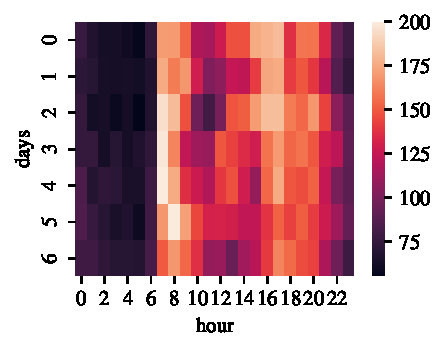
\includegraphics[]{../Figures/LPS/wm_hm_weekly.pdf}
	\label{fig:wm_hm_weekly_2}
\end{figure}

\subsubsection{Bag of Appliances LP}

Another LP that will be used at the end of this Chapter will be the bag-of-appliances LP.
The profile was presented and analyzed in depth in Chapter \ref{chapter4} and was presented in Figure \ref{fig:BOA}.
But again, for ease-of-use purposes, we will summarize the profile here.

\begin{figure}[H]
	\centering
	\caption{Universal presentation of per-building per-appliance LP}
	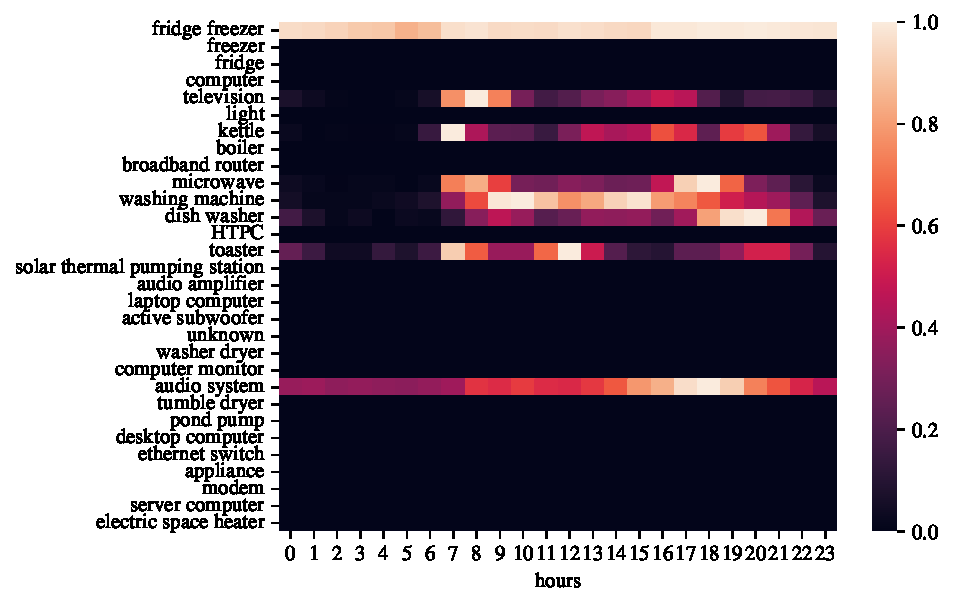
\includegraphics[]{../Figures/LPS/BOA.pdf}
	\label{fig:BOA2}
\end{figure}

To build the profile seen in Figure \ref{fig:BOA2}, we used the data from all 5 datasets and made a list of the most commonly used appliances.
Only the top 30 appliances were selected.
This enables us to have the same LP for all buildings, and thus enables us to see how the usage differs across them.
One problem that arises here is the missing appliances.
These appliances present themselves as a black line.
A lot of missing appliances may cause the image to be primarily black,
which could cause trouble for the algorithm processing this as an image.

\subsection{Data}

We have on average roughly one year of data per building. 
In some cases few weeks and in others up to 5 years for some appliances.
By slicing this data into 1-month-long intervals and converting them to LPs we were able to obtain 5218 samples.

More detailed methodological approaches were discussed in Section \ref{ssec:data}.

\subsection{T-SNE Algorithm}

The t-SNE \cite{tsne2} or t-distribution stochastic neighboring embedding is a method for portraying high dimensional 
data in low dimensional space. This process is also known as dimensionality reduction.

One of the well-known dimensionality reduction algorithms is PCA.
The key difference between the two is that one is linear, and the other is non-linear.
PCA, linear, projects data in new space and finds the one with the least variance between data points.
SNE \cite{sne1}, non-linear, is composed of two main parts. The first one is 
converting the high-dimensional Euclidean distances between data points into conditional probabilities that represent similarities \cite{sne1}.
The pairs with high similarity have a high probability, and pairs with lower a low probability.
Second, it uses Kullback-Leibler divergence to minimize it with respect to a location on a map.
To achieve this it uses gradient descent to minimize the cost function.
Over many iterations, similar data points should be close together and far away from dissimilar objects.
Similar data points usually form clusters. 
t-SNE uses SNE as a basis, except that it uses t-student distribution instead of normal to calculate the similarity.

A good example that showcases the non-linearity of t-SNE can be seen in Figure \ref{fig:tsne_diagram}.
In this simple task, projecting all data points to the y-axis would leave us with a different solution than
one we can see in Figure \ref{fig:tsne_diagram}.
\begin{figure}[H]
    \centering
    \begin{tikzpicture}
        % Draw the input figure
        \node (input) at (0,0) {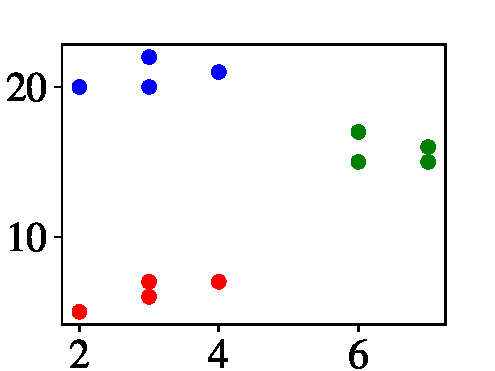
\includegraphics[width=4cm]{Figures/TSNE/DEMO/input.pdf}};
        
        % Draw the output figure
        \node (output) at (6,0) {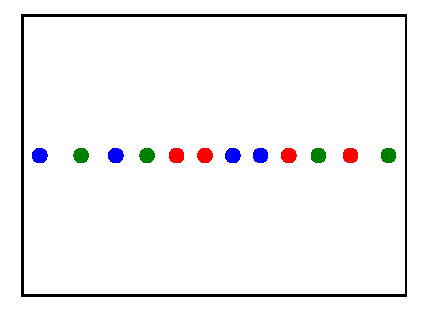
\includegraphics[width=4cm]{Figures/TSNE/DEMO/iteration_4.pdf}};
        
        % Add arrows between the figures
        \draw[->, thick] (input.east) -- (output.west) node[midway, above] {t-SNE};
    \end{tikzpicture}
    \caption{2D data point transformed into 1D data point using t-SNE}
    \label{fig:tsne_diagram}
\end{figure}

In order to calculate the t-SNE for a set of data points, we first need to calculate the conditional probability.
This is calculated based on the Equation \ref{eq:pij} below.
The author of t-SNE Van der Mateen \cite{tsne2} states:
“The similarity of datapoint $x_j$ to datapoint $x_i$ is the conditional probability, $p_{ij}$, that $x_i$ would pick $x_j$ as its neighbor if neighbors were picked in proportion to their probability density under a Gaussian centered at $x_i$.” 

\begin{equation}
\label{eq:pij}
p_{ij} = \frac{\exp(-\lVert x_i - x_j \rVert^2/2\sigma_i^2)}{\sum_{k \neq l} \exp(-\lVert x_k - x_l \rVert^2/2\sigma_i^2)} \
\end{equation}

In Equation \ref{eq:pij} $x_i$ and $x_j$ are two data points and $|x_i - x_j|$ is the Euclidean distance between the two.
The nominator in Equation \ref{eq:pij} is equal to the similarity between two points normalized by the variance $2\sigma_i^2$.
The whole expression is run through $exp()$ function to ensure the value stays positive and within boundaries.
The denominator in Equation \ref{eq:pij} serves as a normalisation factor, to ensure that the sum of probabilities for data point $x_i$ will sum to 1.

The $\sigma_i$ is also known as Gaussian bandwidth, Gaussian kernel or just variance is picked for each data point based on the number of neighbors in its vicinity.
In areas where data points are more crowded, $\sigma_i$ is usually smaller than in less crowded areas.
It is pre-calculated for every point using binary search. 
A search is complete when $\sigma_i$ outputs probability distribution $P_i$ that matches user-defined perplexity $Perp(P_i)$.

$$Perp(P_i) = 2^{H(P_i)}$$

Here, $H(P_i)$ is the entropy of the conditional probability distribution $P_i$.
The entropy of conditional probability distribution is a measure of perplexity.
Perplexity is one of the parameters defined by the user, and it's used as a measure of the number of effective neighbors, between which we will compute similarities.
High perplexity means that the distribution of the Gaussian kernel will be wide and contain more data points between which similarity will be computed.
Low perplexity means that the kernel will be narrow, so fewer data points will fit into it and therefore fewer data points will be compared.

The output of the algorithm is a map of every data point $y_i$.
These points are low dimensional counterparts of $x_i$.
Usually, these data points contain a comprehensible number of dimensions where $y_i \in \mathbb{R}^2$ or $\mathbb{R}^3$. 
Similarly, as in equation \ref{eq:pij} we can now use low dimensional data points $y_i$ and $y_j$ to calculate probability $q_{ij}$ in equation \ref{eq:gij}.
Here, t-student distribution with one degree of freedom is utilized to calculate the similarities.

\begin{equation}
\label{eq:gij}
q_{ij} = \frac{(1+\lVert y_i - y_j \rVert^2)^{-1}}{\sum_{k \neq l} (1+\lVert y_k - y_l \rVert^2)^{-1}} 
\end{equation}

$q_{ij}$ is again a conditional probability of finding $y_i$ and $y_j$ near each other but for fewer dimensions.

Setting up a cost function, which tries to minimize the difference between $q_{ij}$ and $p_{ij}$ should result in a low dimensional map where similar points should be near eachother.
The cost function is also known as Kullback-Leibler divergence seen in Equation \ref{eq:Klle}. 
The equation is the sum of all pairwise similarities between low and high-dimensional data points.
The smaller the $C$ the closer the similar data points are in low dimensional space.

\begin{equation}
\label{eq:Klle}
 C = \sum_{i \neq j}^n p_{ij} \log \frac{p_{ij}}{q_{ij}}
\end{equation}

The similarity is achieved over many iterations where we use gradient descent to minimize the Kullback-Leibler divergence seen in Equation \ref{eq:Klle}. 
The process can be seen in Figure \ref{fig:tsne_iterations_arrows}.

\begin{figure}[H]
    \centering
    \begin{tikzpicture} 
        % Draw the first subfigure
        \node (tsne1) at (0,0) {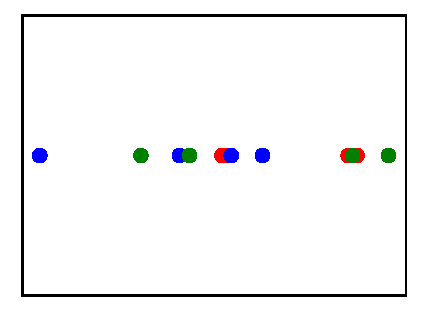
\includegraphics[width=0.25\textwidth]{Figures/TSNE/DEMO/iteration_1.pdf}};
        \node[above] at (tsne1.north) {0 iters};
        
        % Draw the second subfigure
        \node (tsne2) at (0.35\textwidth,0) {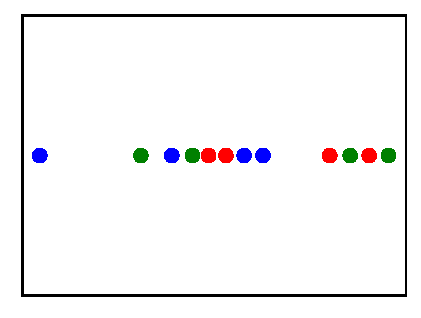
\includegraphics[width=0.25\textwidth]{Figures/TSNE/DEMO/iteration_2.pdf}};
        \node[above] at (tsne2.north) {150 iters};
        
        % Draw the third subfigure
        \node (tsne3) at (0.7\textwidth,0) {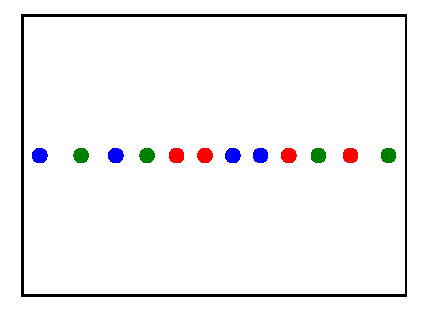
\includegraphics[width=0.25\textwidth]{Figures/TSNE/DEMO/iteration_4.pdf}};
        \node[above] at (tsne3.north) {400 iters};
        
        % Add arrows between the subfigures
        \draw[->, thick] (tsne1.east) -- (tsne2.west);
        \draw[->, thick] (tsne2.east) -- (tsne3.west);
    \end{tikzpicture}
    \caption{Iterations of t-SNE}
	\par
    \par\footnotesize{The input data can be seen in \ref{fig:tsne_diagram} }
	\label{fig:tsne_iterations_arrows}
\end{figure}


In our case, two dimensions will be used. Since this is a non-linear dimensionality reduction,
the axis usually presents dimensions that are hard to comprehend by the brain. 
It is important to keep in mind that the resulting low-dimensional representation is not necessarily interpretable in the same way as the original high-dimensional data.
This also means that the axes labels on the graphical presentations are meaningless.
In our case, we labeled the two axes as $dimension-1$ and $dimension-2$.

\section{Results}

The results will be presented in three subsections

\begin{itemize}
	\item Per-building LP
	\item Per-appliance LP
	\item Per-building per-appliance LP
\end{itemize}

Most of the focus will be done on the per-appliance LP since it is the most universal.

\subsection{Results for Per-Building LPs}
%TODO
\label{ssec:res_pb_lp}
This LP is useful when it comes to comparing how 
activation patterns change over buildings and datasets.
Per-building data uses combined activations of all appliances to present 
the aggregated usage pattern.  

Figure \ref{fig:tsne_scatter_non_norm_all} is using non-normalized data, meaning
the number of appliances in a building will affect the end LP.
The algorithm could pick up on how many appliances are being used.
In some cases, such as energy poverty detection, this information is useful, 
again in othersm, where would like to find more complex usage patterns, we are better off using normalized profiles.

\begin{figure}[H]
	\centering
	\caption{Projection of per-building LPs}
	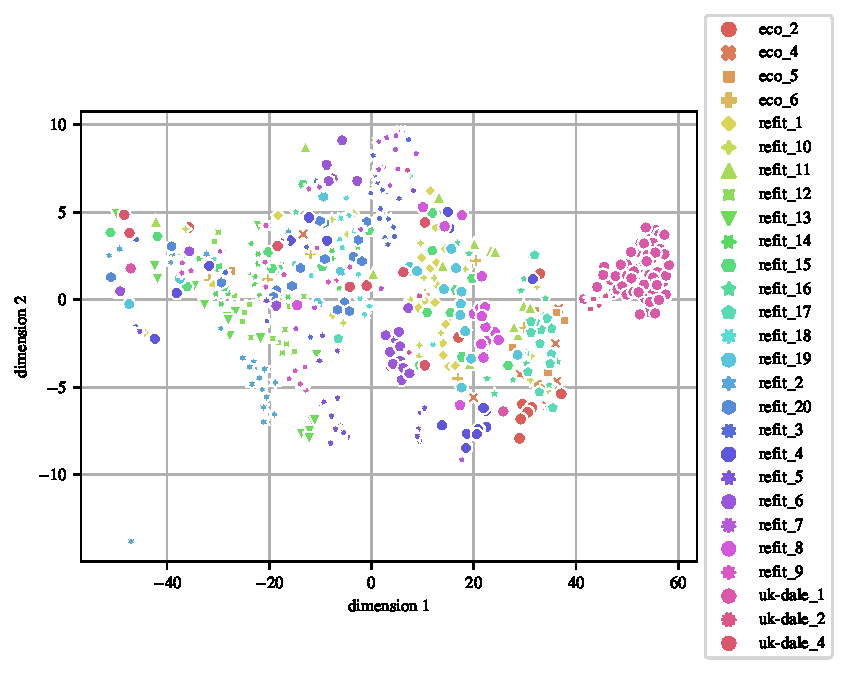
\includegraphics[]{Figures/TSNE/TSNE_per_building/scatter_per_building.pdf}
	\label{fig:tsne_scatter_non_norm_all}
	\par
	\par\footnotesize{Full resolution figure: \url{https://github.com/jenkoj/msc/tree/main/Figures/TSNE/TSNE_per_building/scatter_per_building.pdf}}
\end{figure}

Figure \ref{fig:tsne_pb_img_scatter_allall} below presents the actual LP for each sample. 
It is possible to see that on the left there are mostly samples with very little activity,
and on the right, we see samples with more activity.
Since the two plotted components are of a higher dimension, it is hard to determine what they present.
As said t-SNE gives us the intuition of how LPs are connected in higher-dimensional space.

The following figures are best viewed in color and a digital format. 
Readers reading the digital version should have the ability to zoom into each cluster, and see the actual samples. 
Readers reading a paper version can still explore the high-resolution figures online via the provided link below every figure.

\begin{figure}[H]
	\centering
	\caption{Projection of per-building LPs with actual samples}
	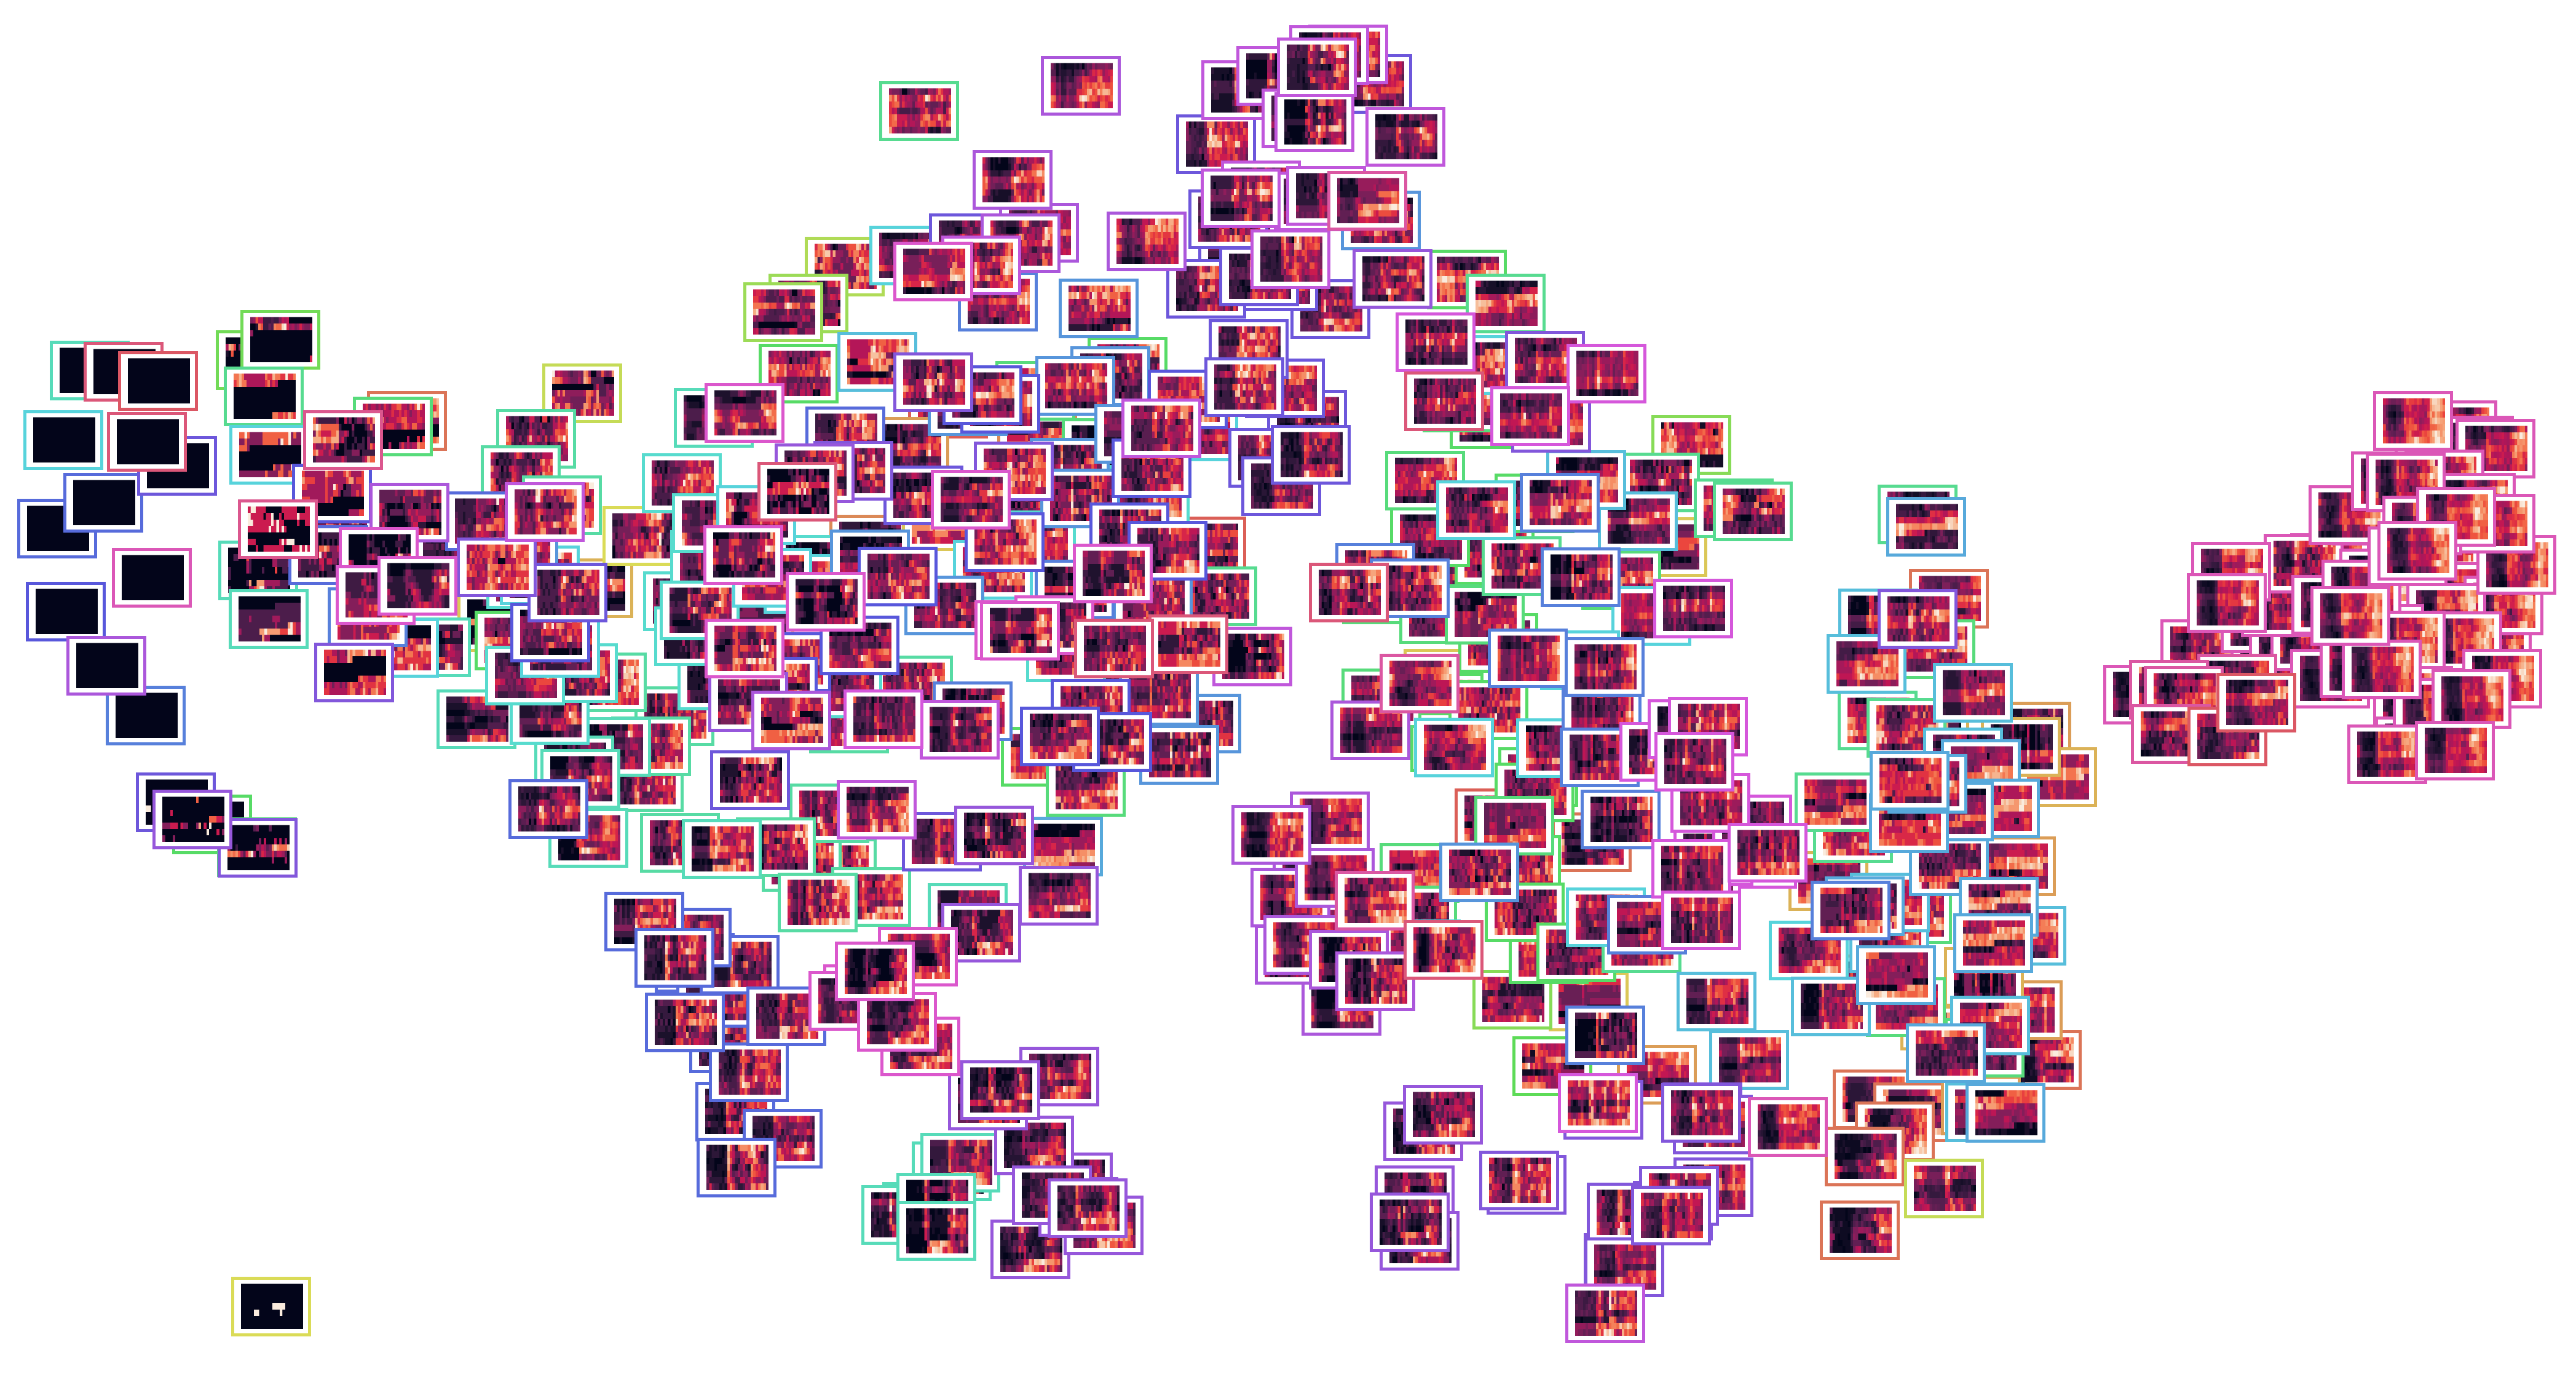
\includegraphics[width=.9\textwidth]{Figures/TSNE/TSNE_per_building/img_scatter_per_building.png}
	\label{fig:tsne_pb_img_scatter_allall}
	\par
	\par\footnotesize{Full resolution figure: \url{https://github.com/jenkoj/msc/tree/main/Figures/TSNE/TSNE_per_building/img_scatter_per_building.png}}
\end{figure}

\subsubsection{Normalized LPs}

To solve the issue mentioned in Subsection \ref{ssec:res_pb_lp} have to normalize the data between 0 and 1.
Figure \ref{fig:tsne_pb_scatter_all_all} shows how normalizing samples affect the algorithm.

When comparing figures \ref{fig:tsne_scatter_non_norm_all} and \ref{fig:tsne_pb_scatter_all_all},
it is possible to see that the samples on the latter are much closer to each other,
while it is still possible to see the individual clusters.
This could imply that the normalized usage pattern of users is more similar to the activation pattern of users.
A normalized activation pattern tells us at what part of the day the appliances will most likely be used,
and the activation pattern tells us how much will the appliance be used in each part of the day.
Based on that, we can conclude the time when the appliance is used is more consistent than how much it will be used. 


\begin{figure}[H]
	\centering
	\caption{Projection of normalised per-building LPs}
	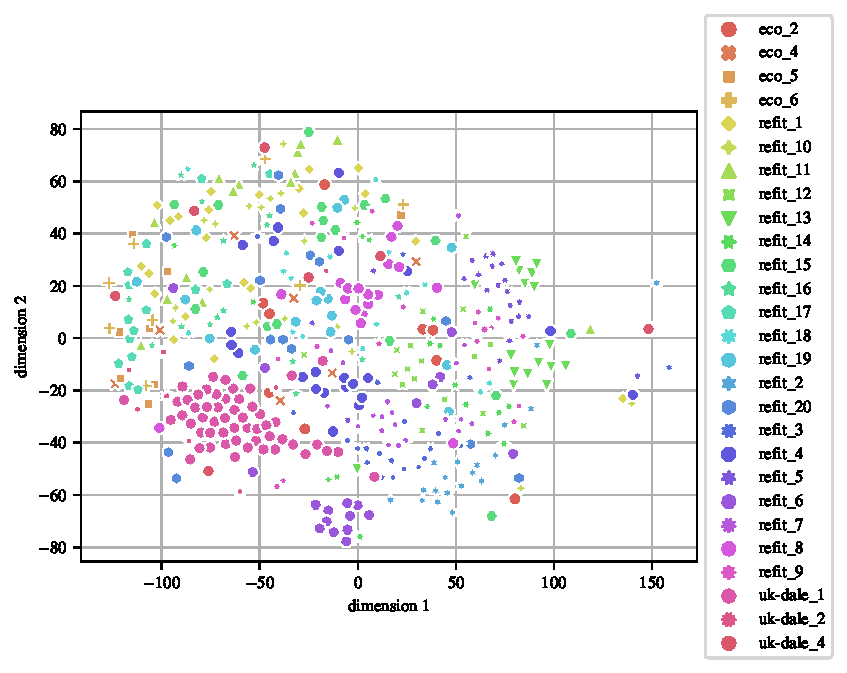
\includegraphics[]{Figures/TSNE/TSNE_per_building/scatter_per_building_norm.pdf}
	\label{fig:tsne_pb_scatter_all_all}
	\par
	\par\footnotesize{Full resolution figure: \url{https://github.com/jenkoj/msc/tree/main/Figures/TSNE/TSNE_per_building/scatter_per_building_norm.pdf}}
\end{figure}

Figure \ref{fig:tsne_pb_img_norm_scatter_allall} presents only the main cluster of samples.
Since the smaller cluster presents mostly low entropy data, it was cut out. 
If the reader wants to see the samples in the cluster, the very same cluster can be found on the far left in Figure \ref{fig:tsne_pb_img_scatter_allall}.

\begin{figure}[H]
	\centering
	\caption{Projection of normalised per-building LPs with actual samples}
	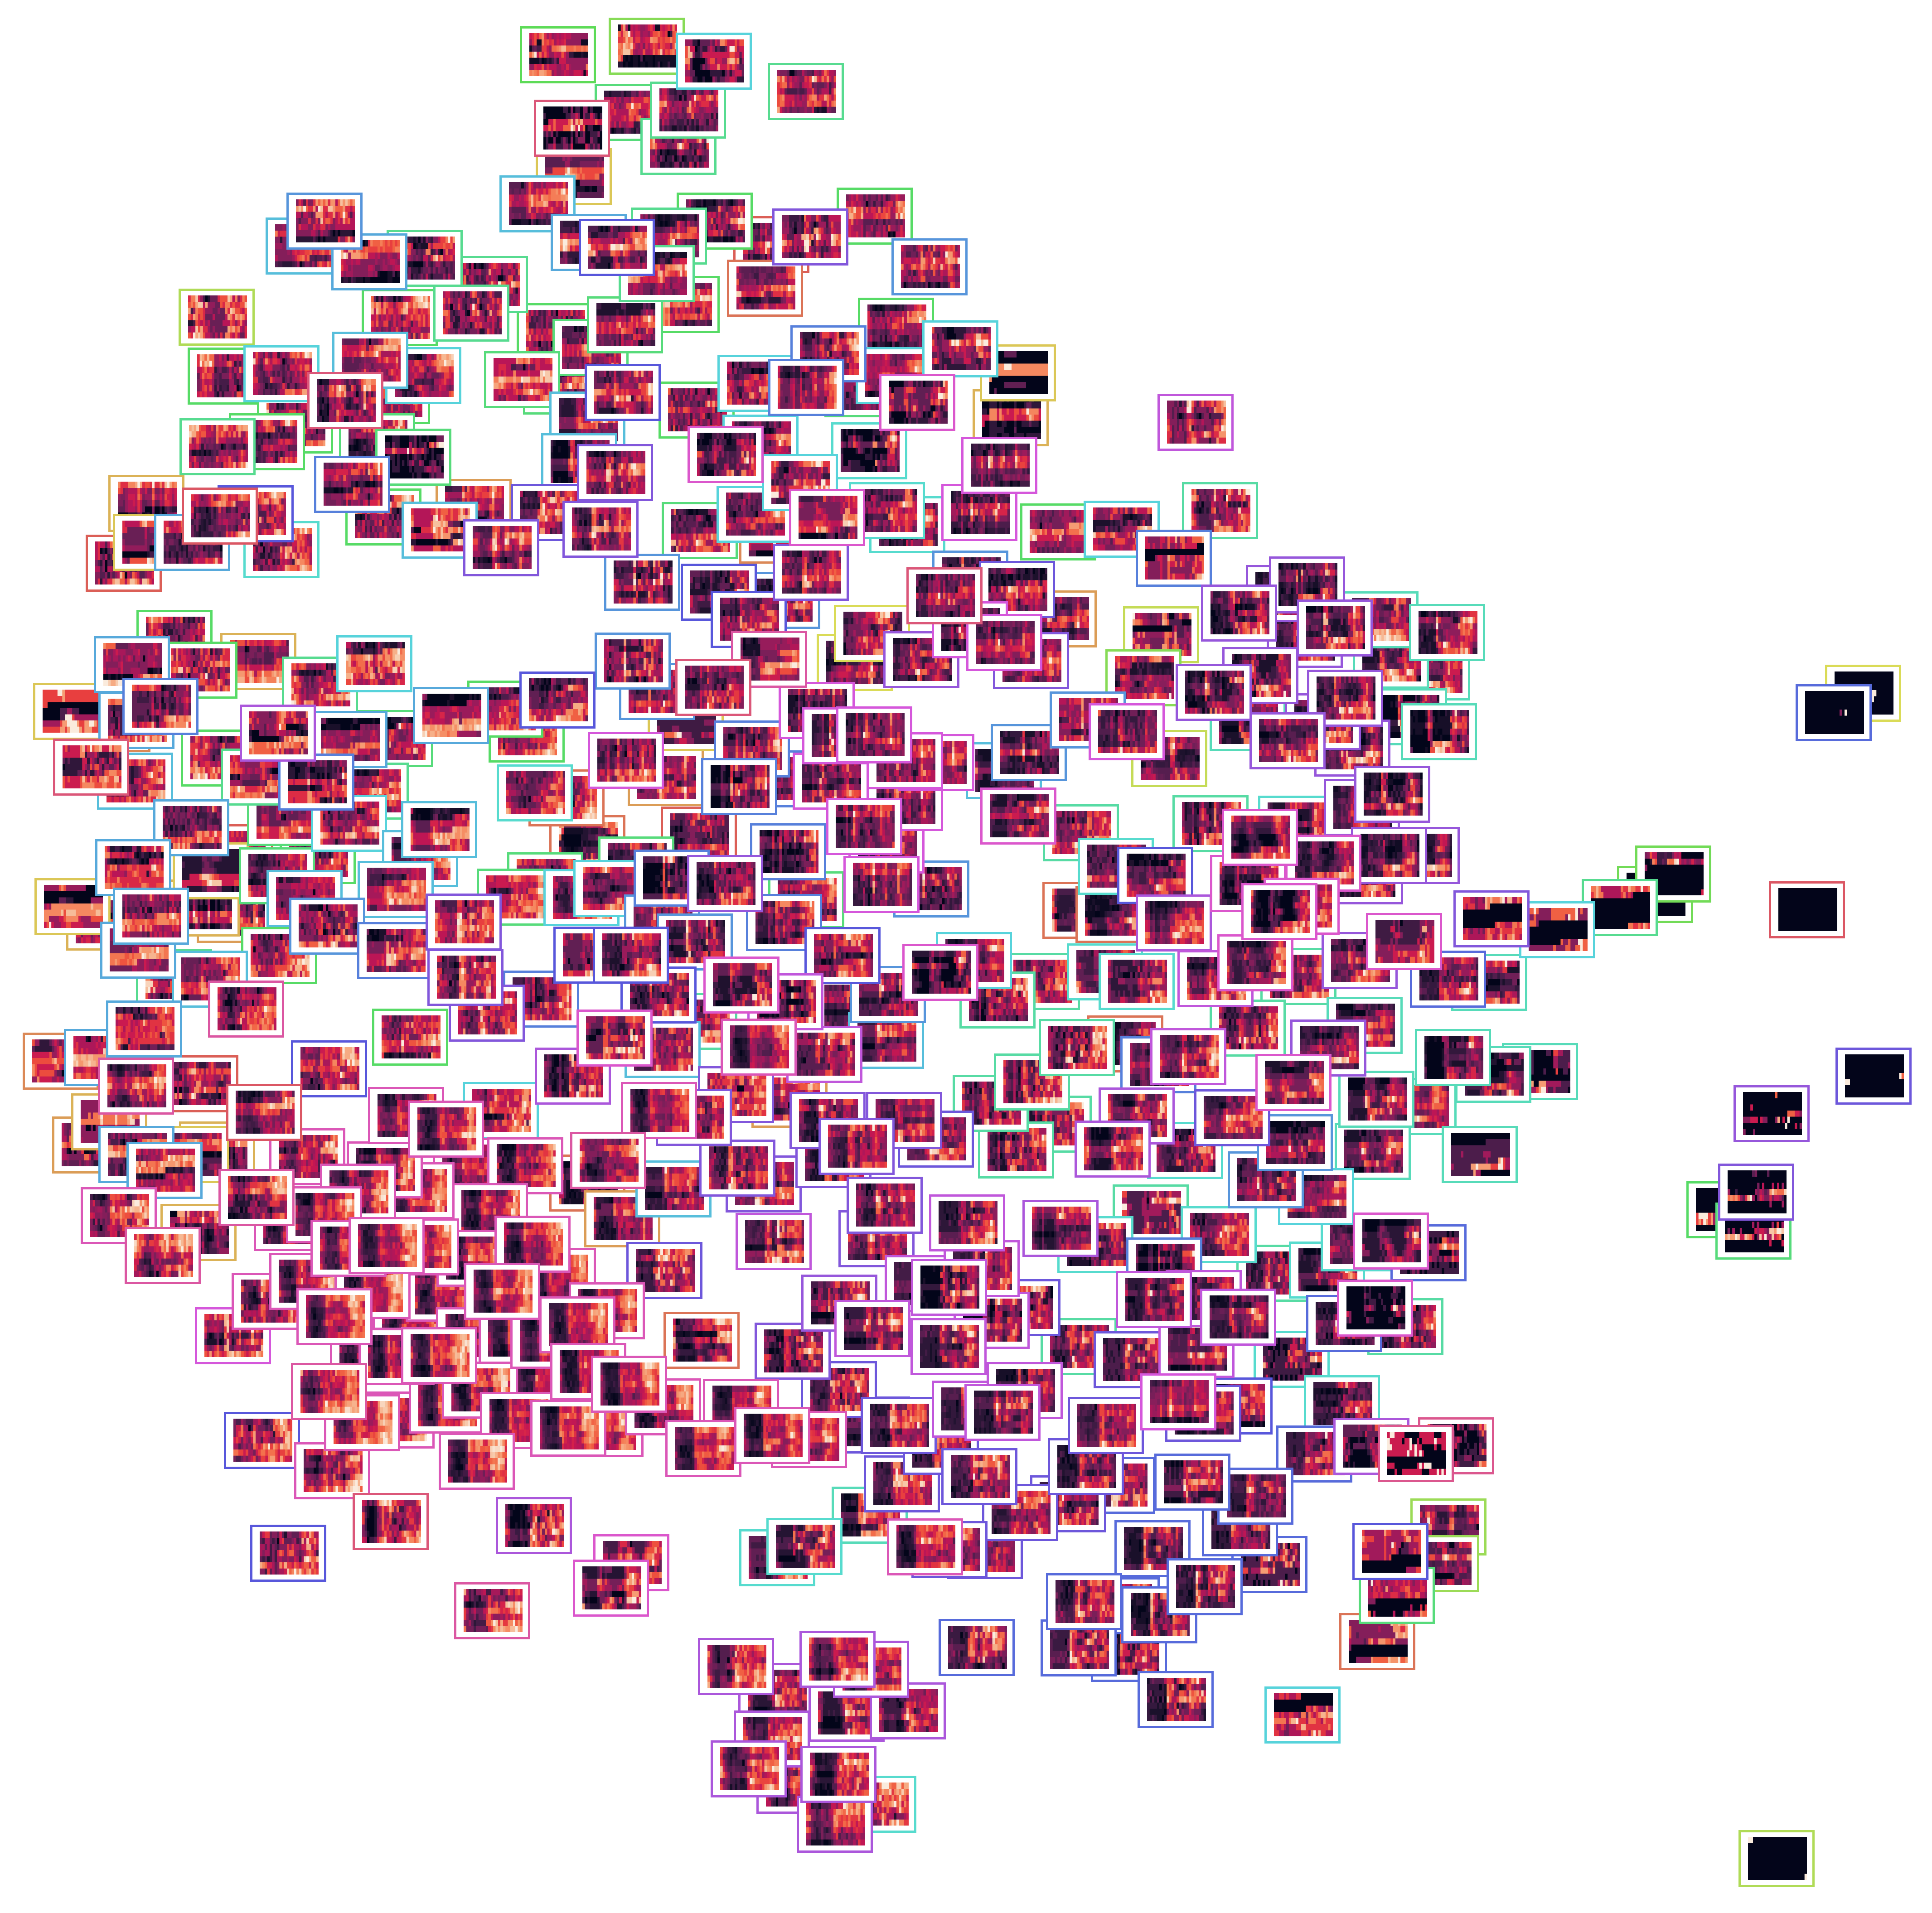
\includegraphics[width=.9\textwidth]{Figures/TSNE/TSNE_per_building/img_scatter_per_building_norm.png}
	\label{fig:tsne_pb_img_norm_scatter_allall}
	\par
	\par\footnotesize{Full resolution figure: \url{https://github.com/jenkoj/msc/tree/main/Figures/TSNE/TSNE_per_building/img_scatter_per_building_norm.png}}
\end{figure}

In Figure \ref{fig:tsne_pb_img_norm_scatter_allall} it is possible to find various usage patterns. 
But the general pattern is that there is less activity during the night with one peak in the morning and evening hours.
Some buildings are more active during the week and again some more during the weekend.
A lot of the data is from UK-DALE building 1 (pink box). 
It is possible to see that the building has one big cluster where activations are generally similar, with few outliers, where the pattern completely changed. 
Albeit less obvious, this pattern is the same for all buildings.
This happens due to events such as vacations, holidays or weather-induced behavioral changes.

\subsection{Per-Appliance}

We can use per-appliance LPs to examine how different appliances 
are used in a single building, how a single appliance is being used across other buildings or how many appliances are being used in many buildings.

Per appliance LPs are built using sub-meter data,
meaning each LP should present each appliance.

\subsubsection{Single Appliance Over Many Buildings}

Using one appliance and the building as a label,
allows us to examine how the same type of appliance is being used across different buildings.

Fridges are generally a bad indicator when it comes to user behavior since the user does not affect its operation. 
The only case when the user interacts with it is when opening the door and turning on the light inside. 
Usually, this event is dwarfed by the activations of a compressor. 
This also means that the usage pattern should be the same across all buildings. 
This can be seen in Figure \ref{fig:tsne_pa_scatter_all_fridge}, 
where apart from REFIT buildings 1 and 11, there are no clusters.


\begin{figure}[H]
	\centering
	\caption{Projection of fridge LPs for various buildings}
	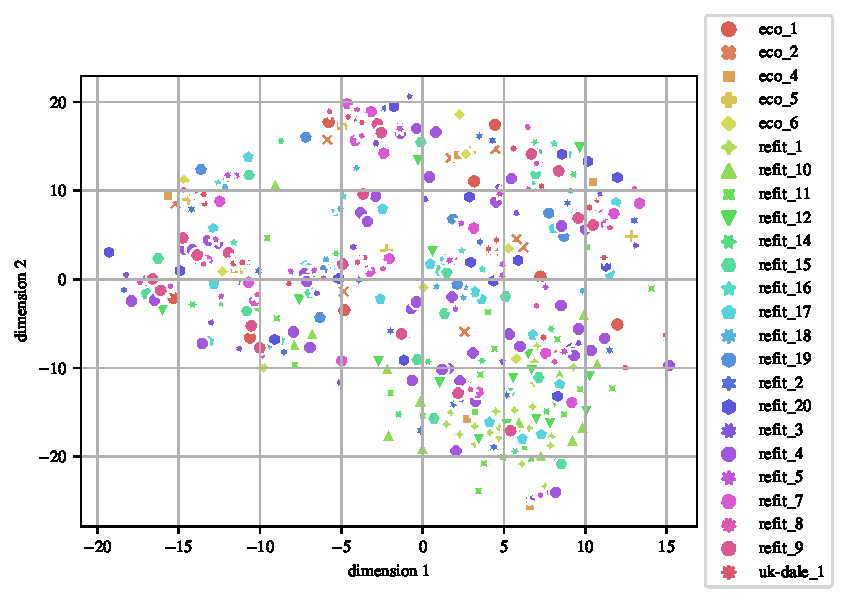
\includegraphics[]{Figures/TSNE/TSNE_per_appliance/scatter_refit_fridge_freeezer_fridge_freezer.pdf}
	\label{fig:tsne_pa_scatter_all_fridge}
	\par
	\par\footnotesize{Full resolution figure: \url{https://github.com/jenkoj/msc/tree/main/Figures/TSNE/TSNE_per_appliance/scatter_refit_fridge_freeezer_fridge_freezer.pdf}}
\end{figure}

Figure \ref{fig:tsne_pa_img_scatter_all_fridge} Shows mostly bright images, apart from a few outliers.
LPs scattered in a circle are generally less dynamic than the ones at the bottom.
Figure \ref{fig:tsne_pa_img_scatter_all_fridge} is a good example of how LPs with little to no human interaction, can look a lot different. 
This could be due to different makes of the appliances, malfunctions of the appliance or the meter measuring it.

\begin{figure}[H]
	\centering
	\caption{Projection of fridge LPs for various buildings with actual samples}
	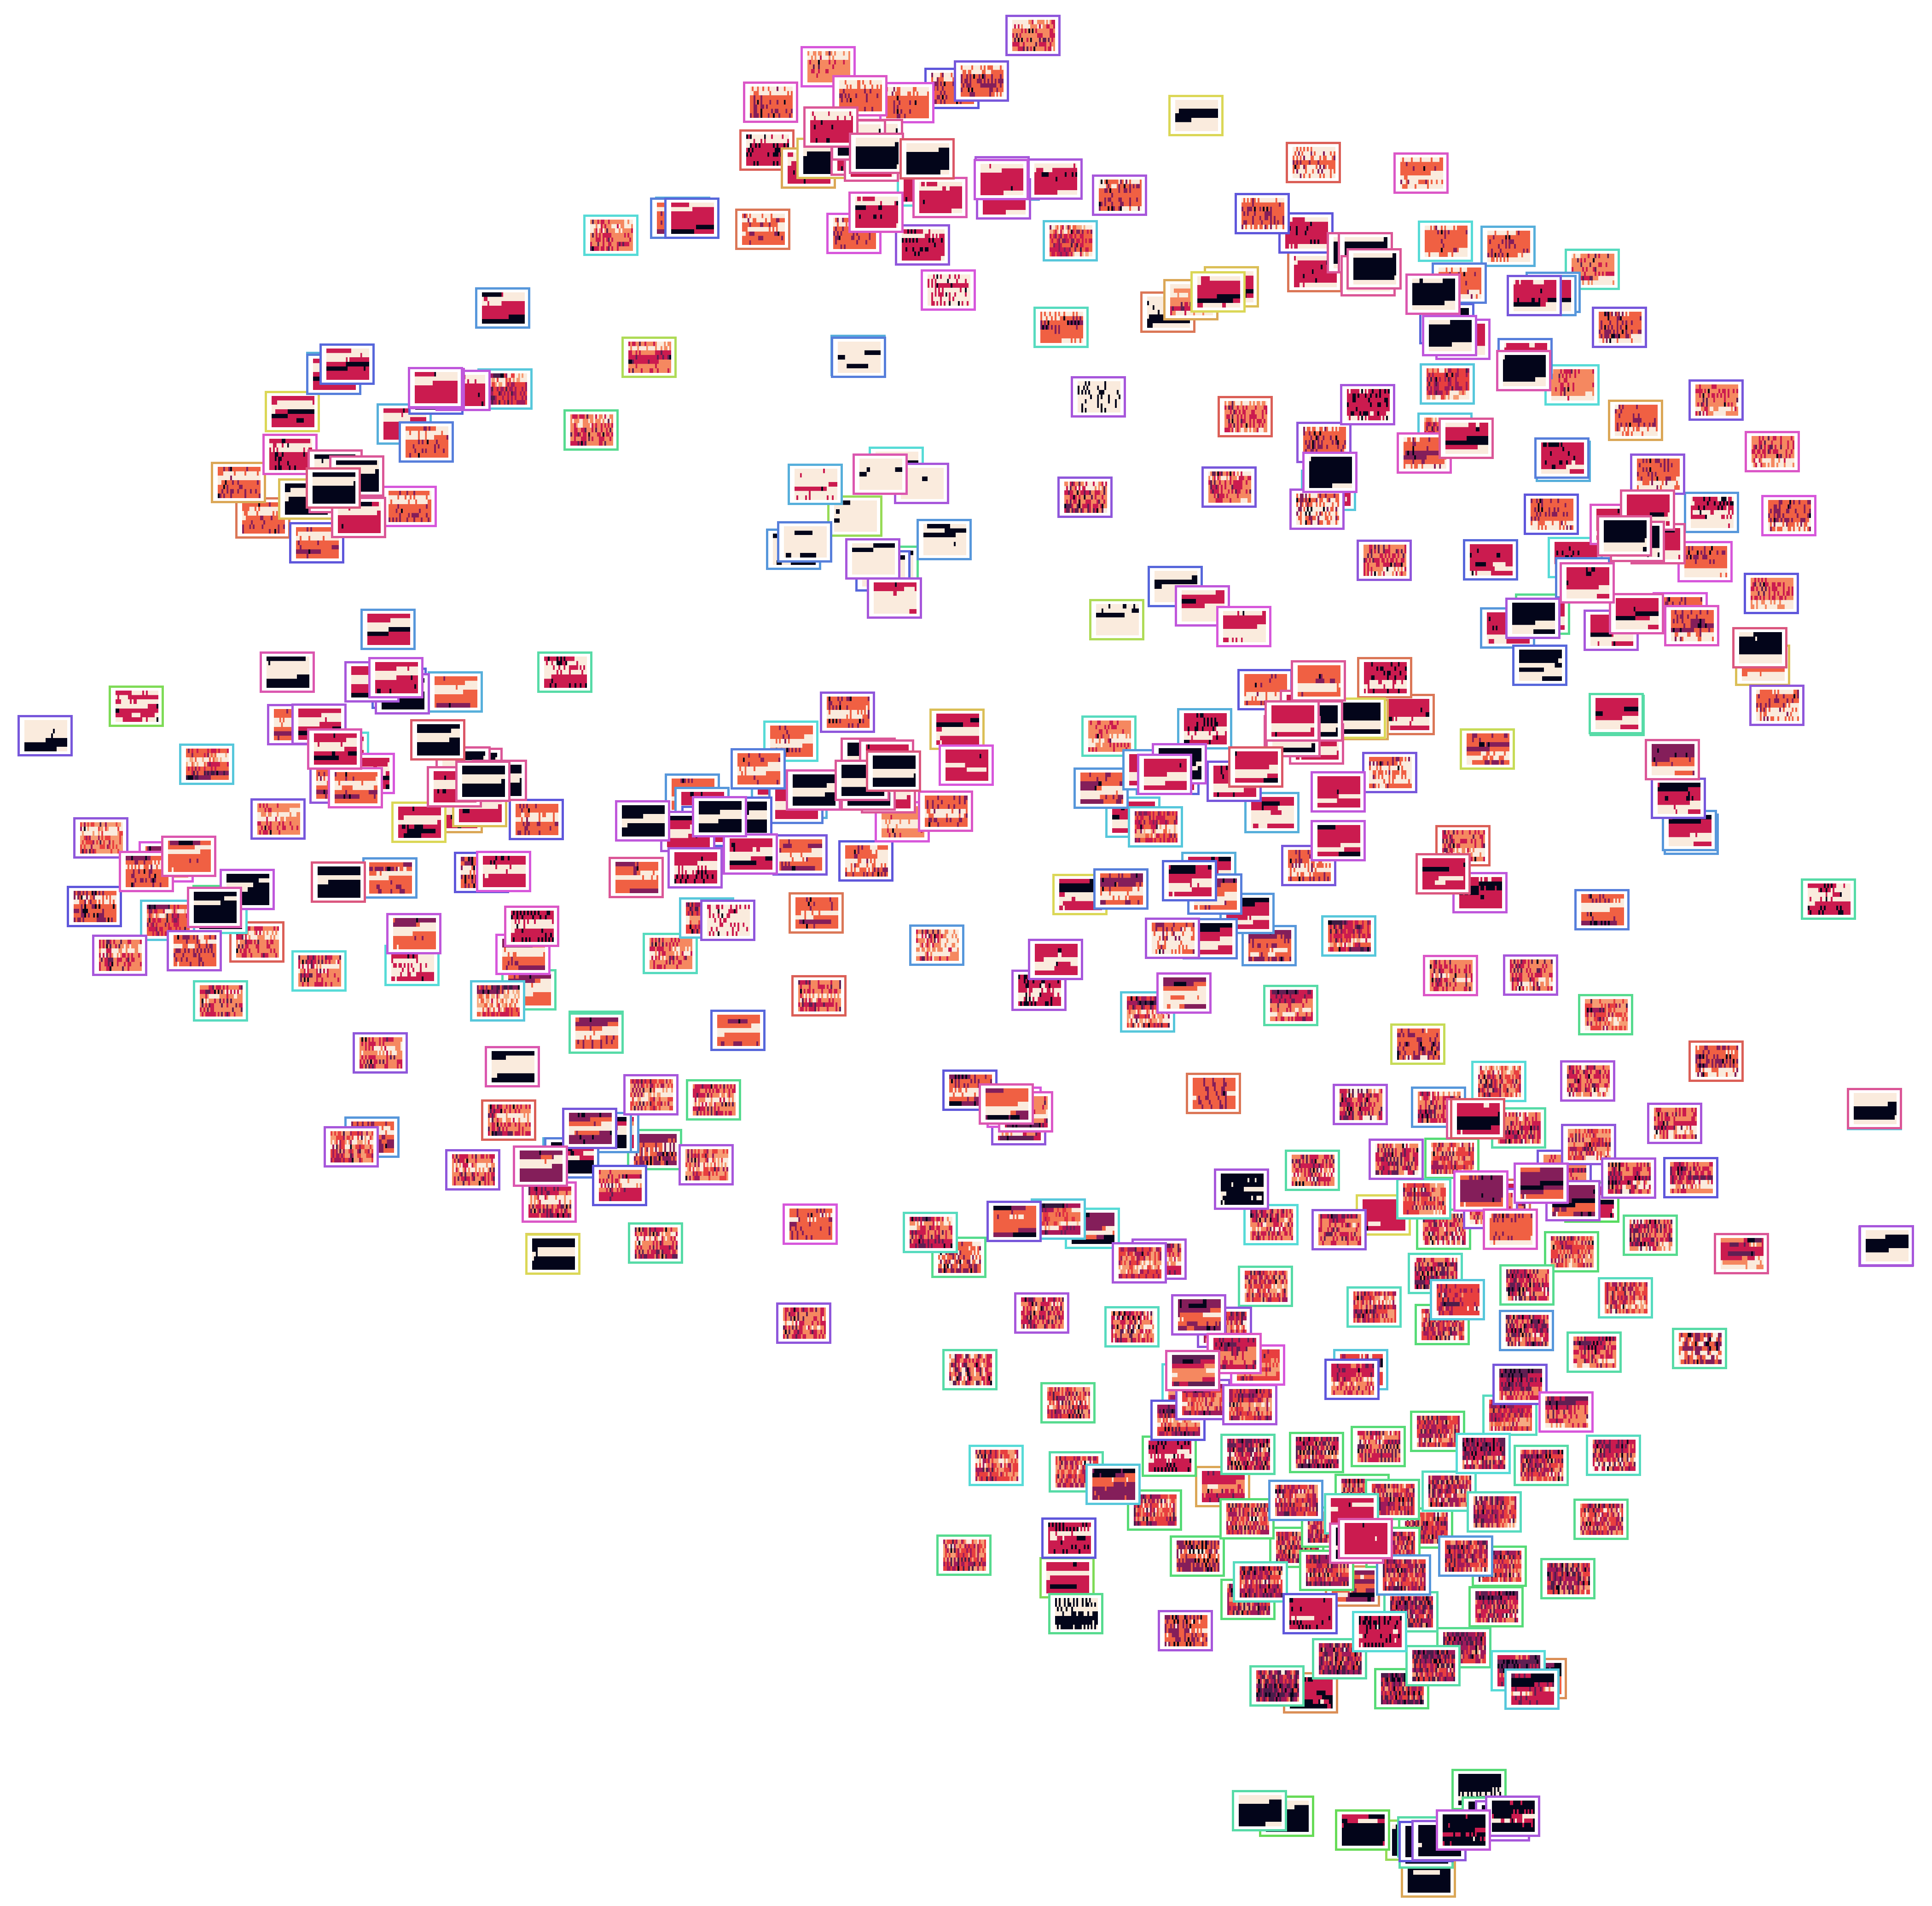
\includegraphics[width=.9\textwidth]{Figures/TSNE/TSNE_per_appliance/img_scatter_refit_fridge_freeezer_fridge_freezer.png}
	\label{fig:tsne_pa_img_scatter_all_fridge}
	\par
	\par\footnotesize{Full resolution figure: \url{https://github.com/jenkoj/msc/tree/main/Figures/TSNE/TSNE_per_appliance/img_scatter_refit_fridge_freeezer_fridge_freezer.png}}
\end{figure}

Figure \ref{fig:tsne_pa_scatter_all_kettle} shows how,
compared to fridges, kettles have many clear clusters that are spaced out between each other. 
This could mean that every household uses a kettle a bit differently.
This cluster is a good example where we can see how strong is a routine of a user.
The closer together the clusters, the higher the routine since samples are more similar to each other.

\begin{figure}[H]
	\centering
	\caption{Projection of kettle LPs for various buildings}
	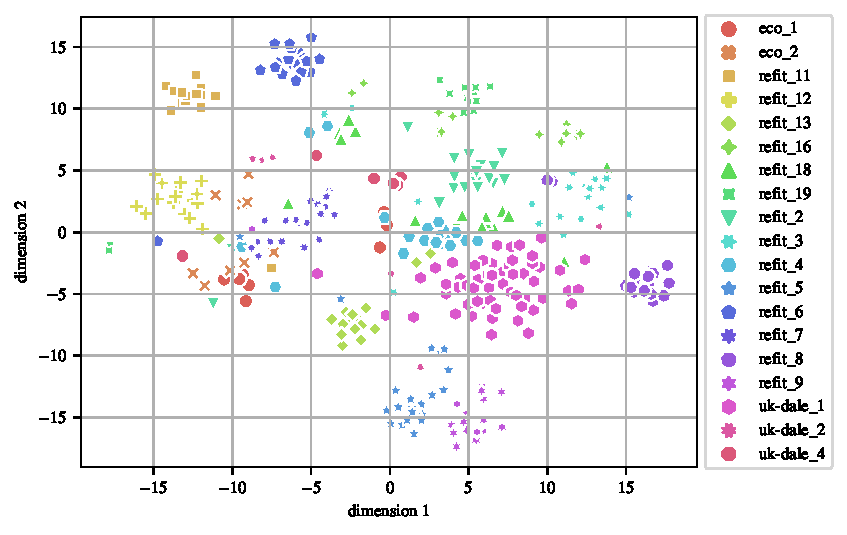
\includegraphics[]{Figures/TSNE/TSNE_per_appliance/scatter_refit_kettle.pdf}
	\label{fig:tsne_pa_scatter_all_kettle}
	\par
	\par\footnotesize{Full resolution figure: \url{https://github.com/jenkoj/msc/tree/main/Figures/TSNE/TSNE_per_appliance/scatter_refit_kettle.pdf}}
\end{figure}

Figure \ref{fig:tsne_pa_img_scatter_all_kettle} shows us that images on the lower part 
of the plot contain less activity than the others. 
LPs that are closer together have more similar activation patterns.
Similar activation patterns are caused by similar behavior, which is essentially a routine.
This means that this projection could be used to calculate how much a behavior variates in time for each building.
This could be calculated by measuring the scattering of samples (variance) for each building.

If we find samples that always activate in the same morning buckets, we would see that they form a straight line on the y-axis.
This is the daily routine. One such example can be seen in Figure \ref{fig:tsne_pa_scatter_all_kettle} in cluster refit 5 and refit 9, where we can see the lines and the pattern throughout the day. 
Since the routine is present, the samples look more similar and are therefore closer together. 
This does not necessarily mean that the closer the samples higher the routine.
They could also be together in case of "ordered chaos" such as can be seen in Figure \ref{fig:tsne_pa_scatter_all_kettle} for building refit 16 and refit 8 where there is no pattern through the day.
So the scattering is not a precise metric when it comes to the routine, but it gives us a rough idea of its presence.
The strength of a routine is an important feature that will be used
in Chapter \ref{chapter6} to build an elderly care anomaly system.

\begin{figure}[H]
	\centering
	\caption{Projection of kettle LPs for various buildings with actual samples}
	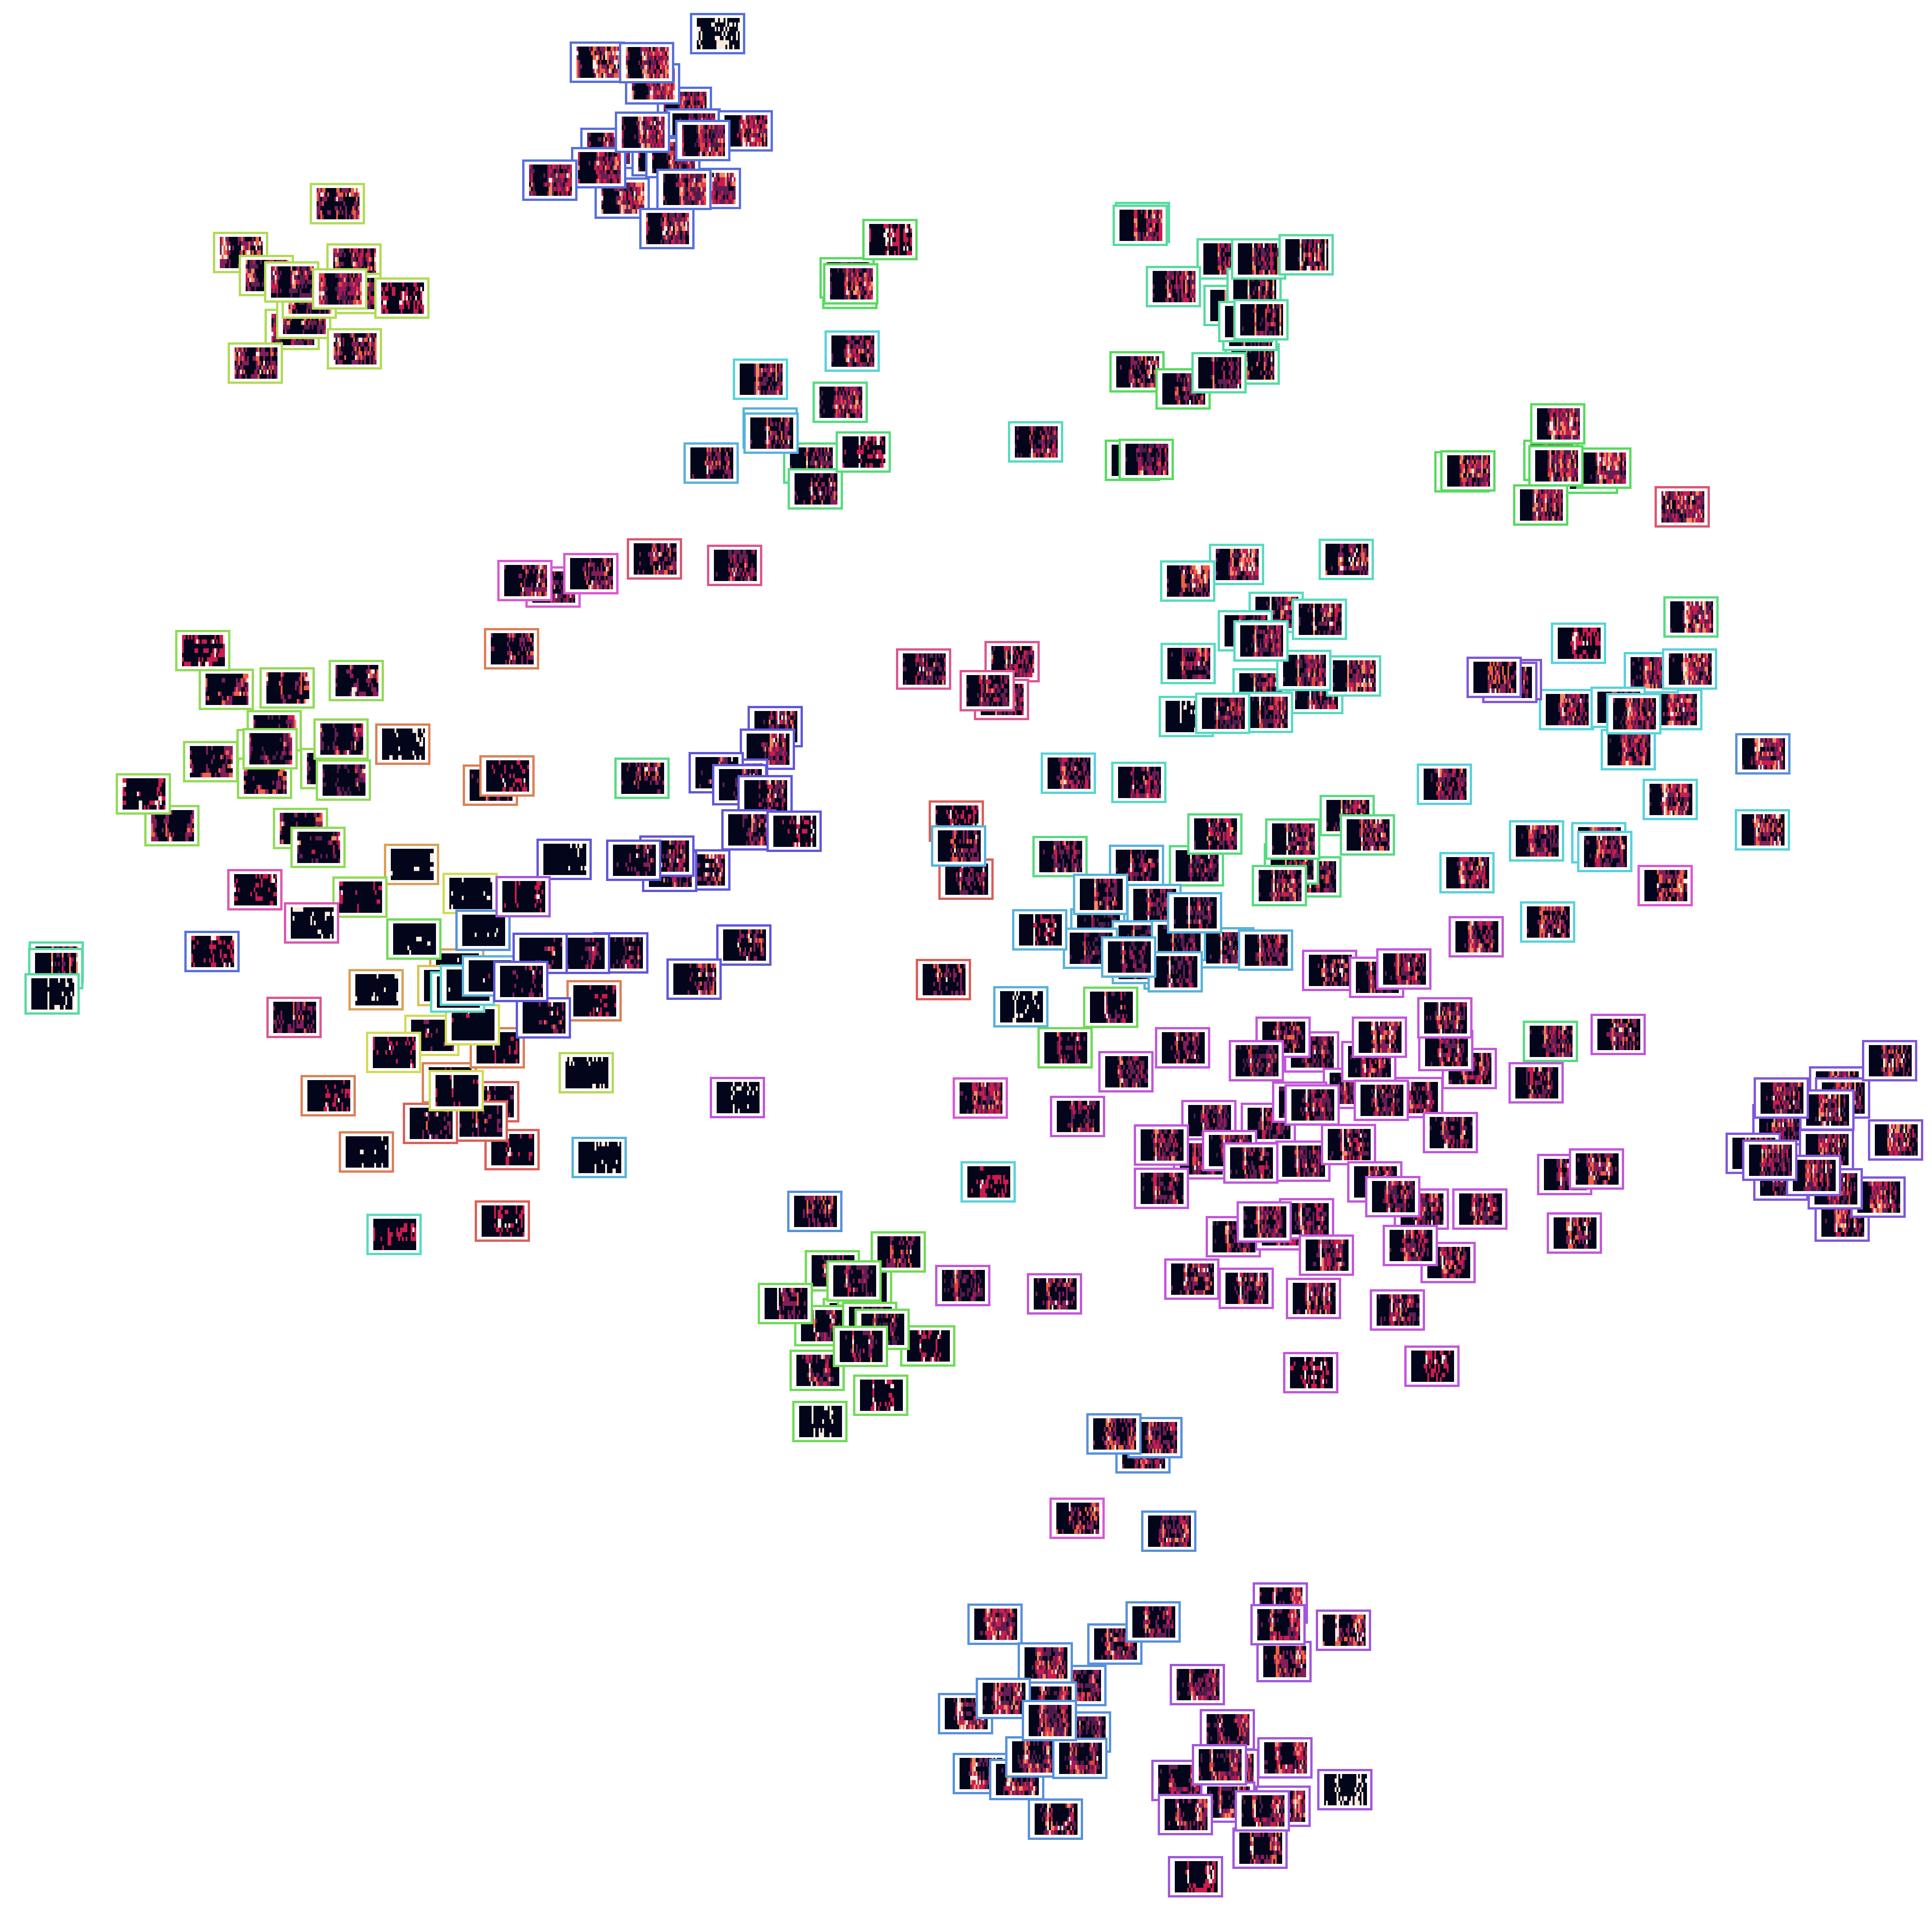
\includegraphics[width=.9\textwidth]{Figures/TSNE/TSNE_per_appliance/img_scatter_refit_kettle.png}
	\label{fig:tsne_pa_img_scatter_all_kettle}
	\par
	\par\footnotesize{Full resolution figure: \url{https://github.com/jenkoj/msc/tree/main/Figures/TSNE/TSNE_per_appliance/img_scatter_refit_kettle.png}}
\end{figure}

% Figure \ref{fig:tsne_pa_scatter_all_microwave} shows that microwaves are again a bit different from the kettle.
% They are more clustered than the fridges, and less than the kettles, even though they are used similarly.
% This could be due to additional electronics such as a clock that are built into
% the appliance. This could lead to some samples being registered as turned on due to 
% a "dark" current. One other difference between the two is that microwave has more than one mode of operation.

% \begin{figure}[H]
% 	\centering
% 	\caption{Projection of microwave LPs for various buildings}
% 	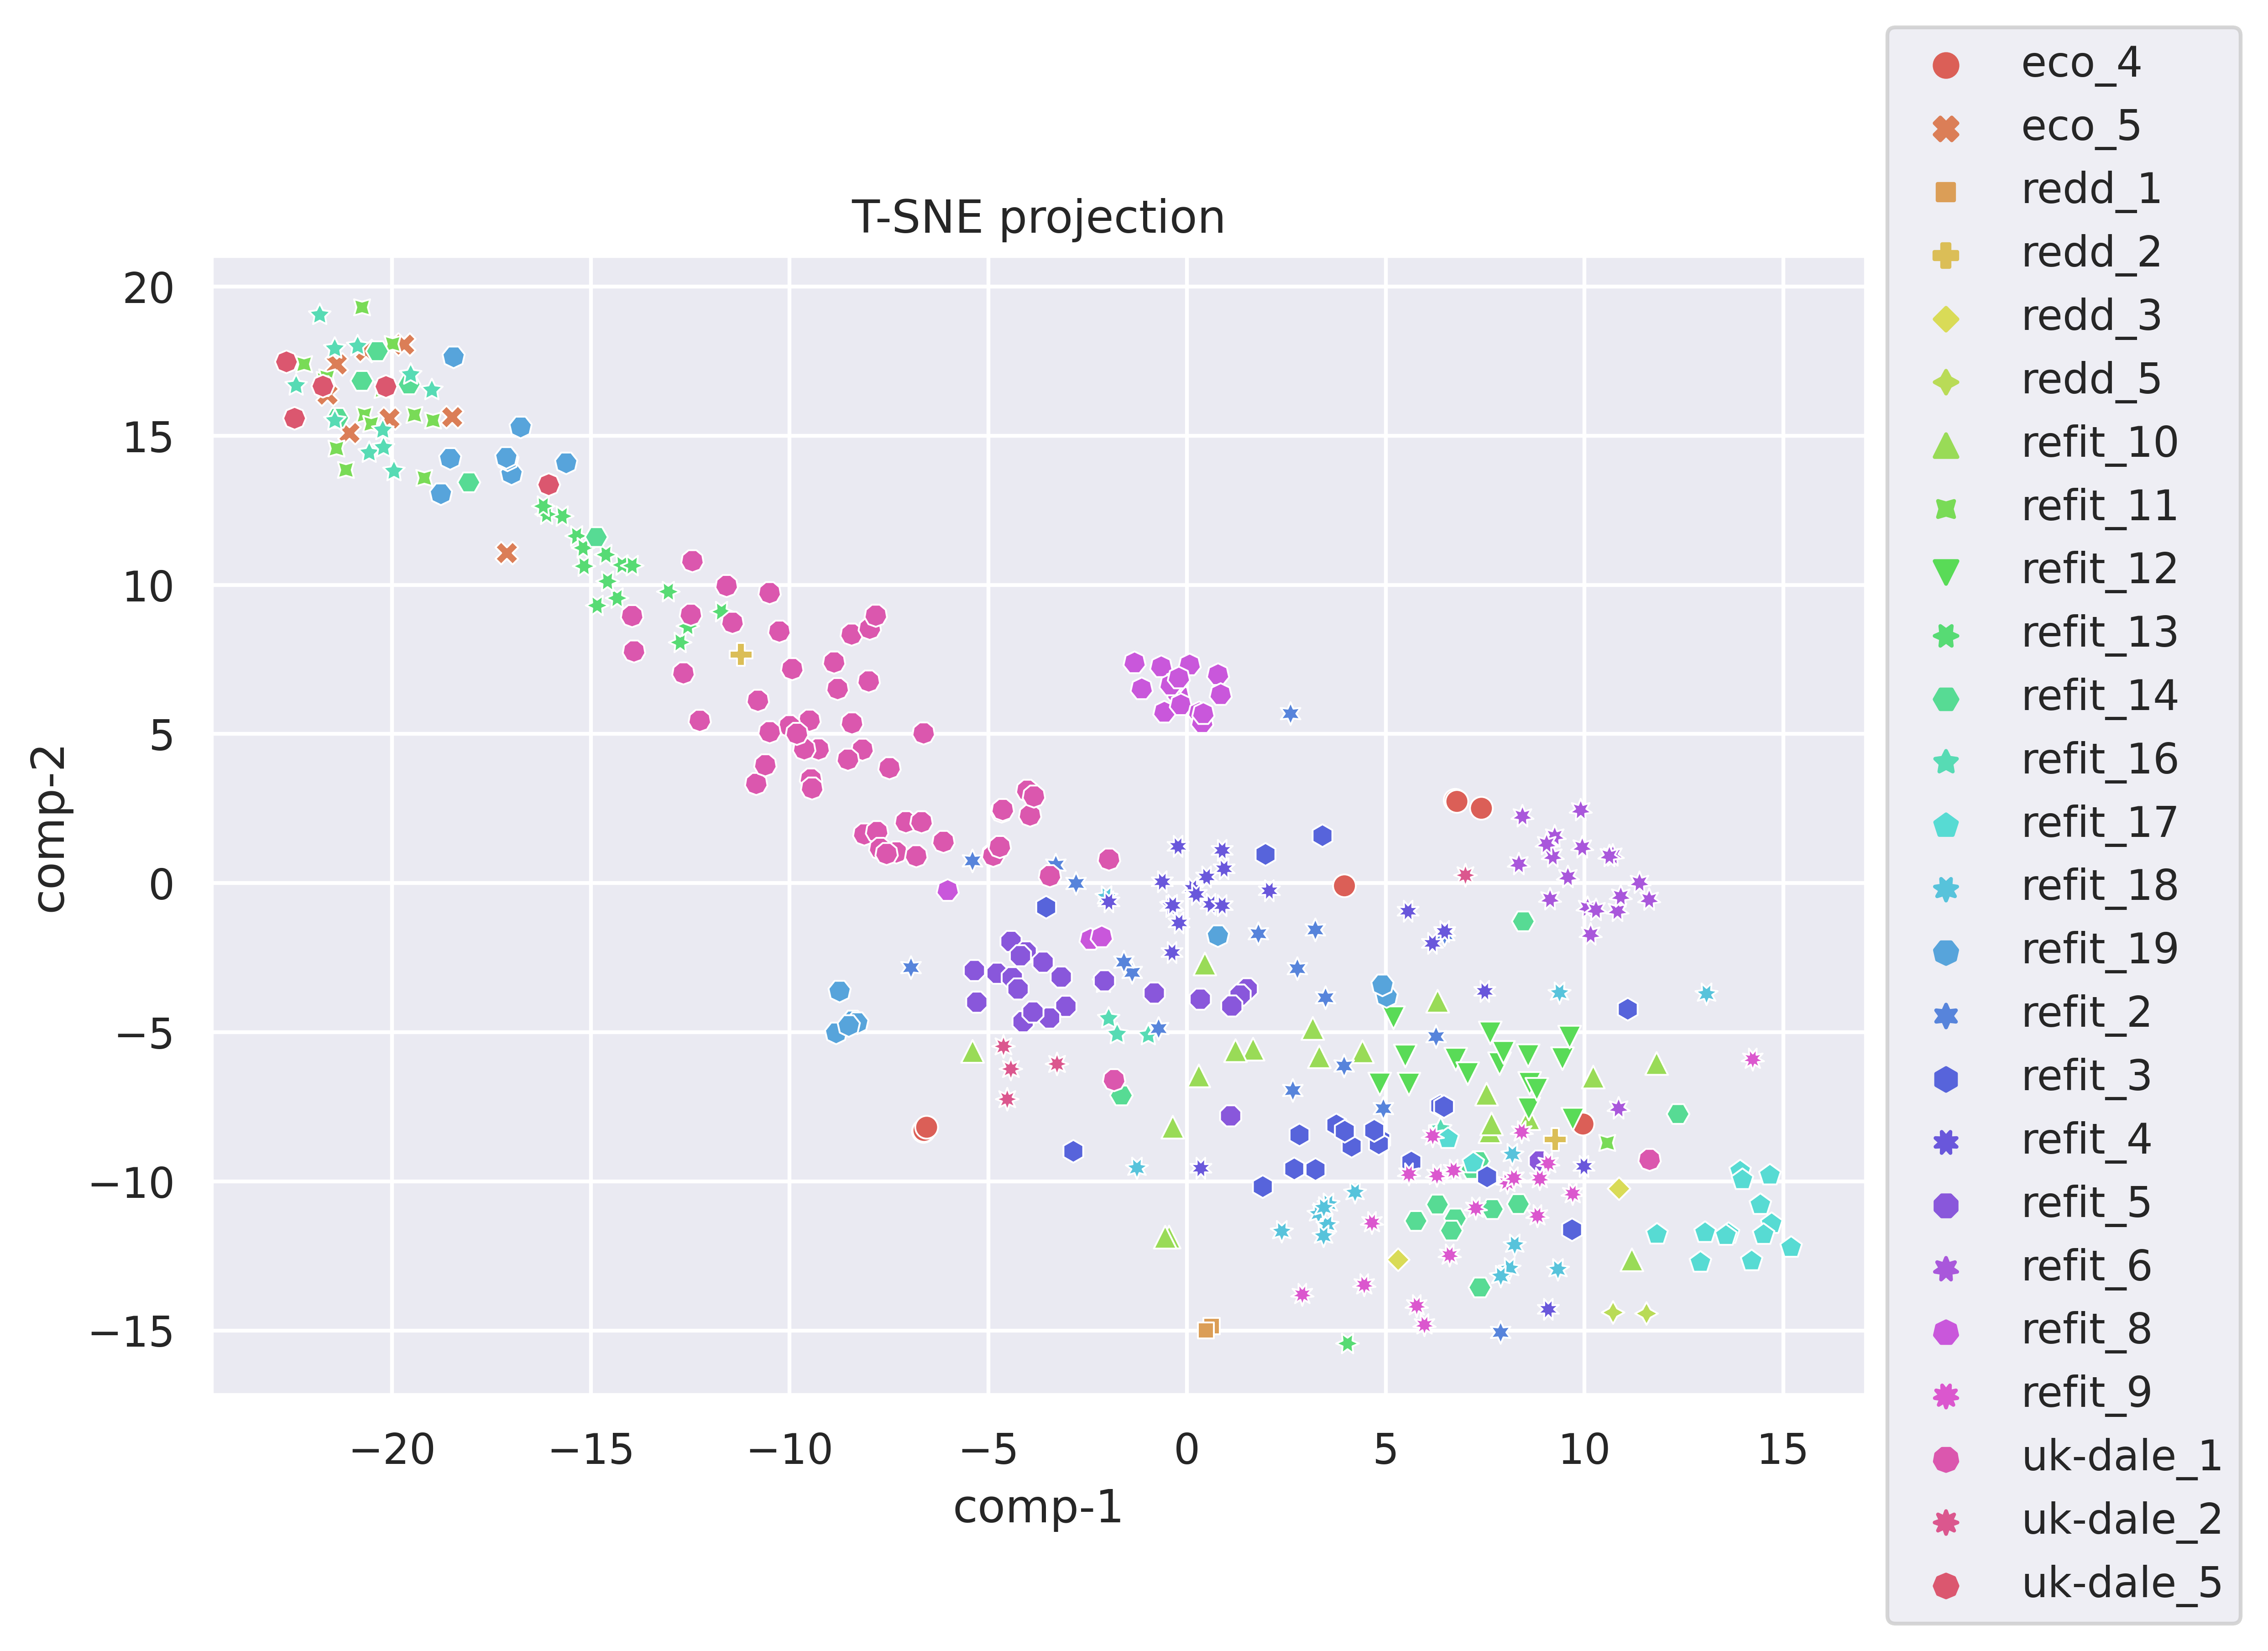
\includegraphics[width=1.2\textwidth]{Figures/TSNE/TSNE_per_appliance/all/scatter_all_microwave.png}
% 	\label{fig:tsne_pa_scatter_all_microwave}
% \end{figure}

% Figure \ref{fig:tsne_pa_img_scatter_all_microwave} shows the faulty samples could be the ones in the upper left part of the plot since they are too bright.
% They do present a pattern, but it is questionable what it presents since it seems like it's turned on during the nighttime. 
% Images at the other end show less lot less activity, which could indicate that
% the household does not use microwaves as much. The most interesting LPs are in the middle of the 
% plot, where it is possible to observe clear activation patterns. 

% \begin{figure}[H]
% 	\centering
% 	\caption{Projection of microwave LPs for various buildings with actual samples}
% 	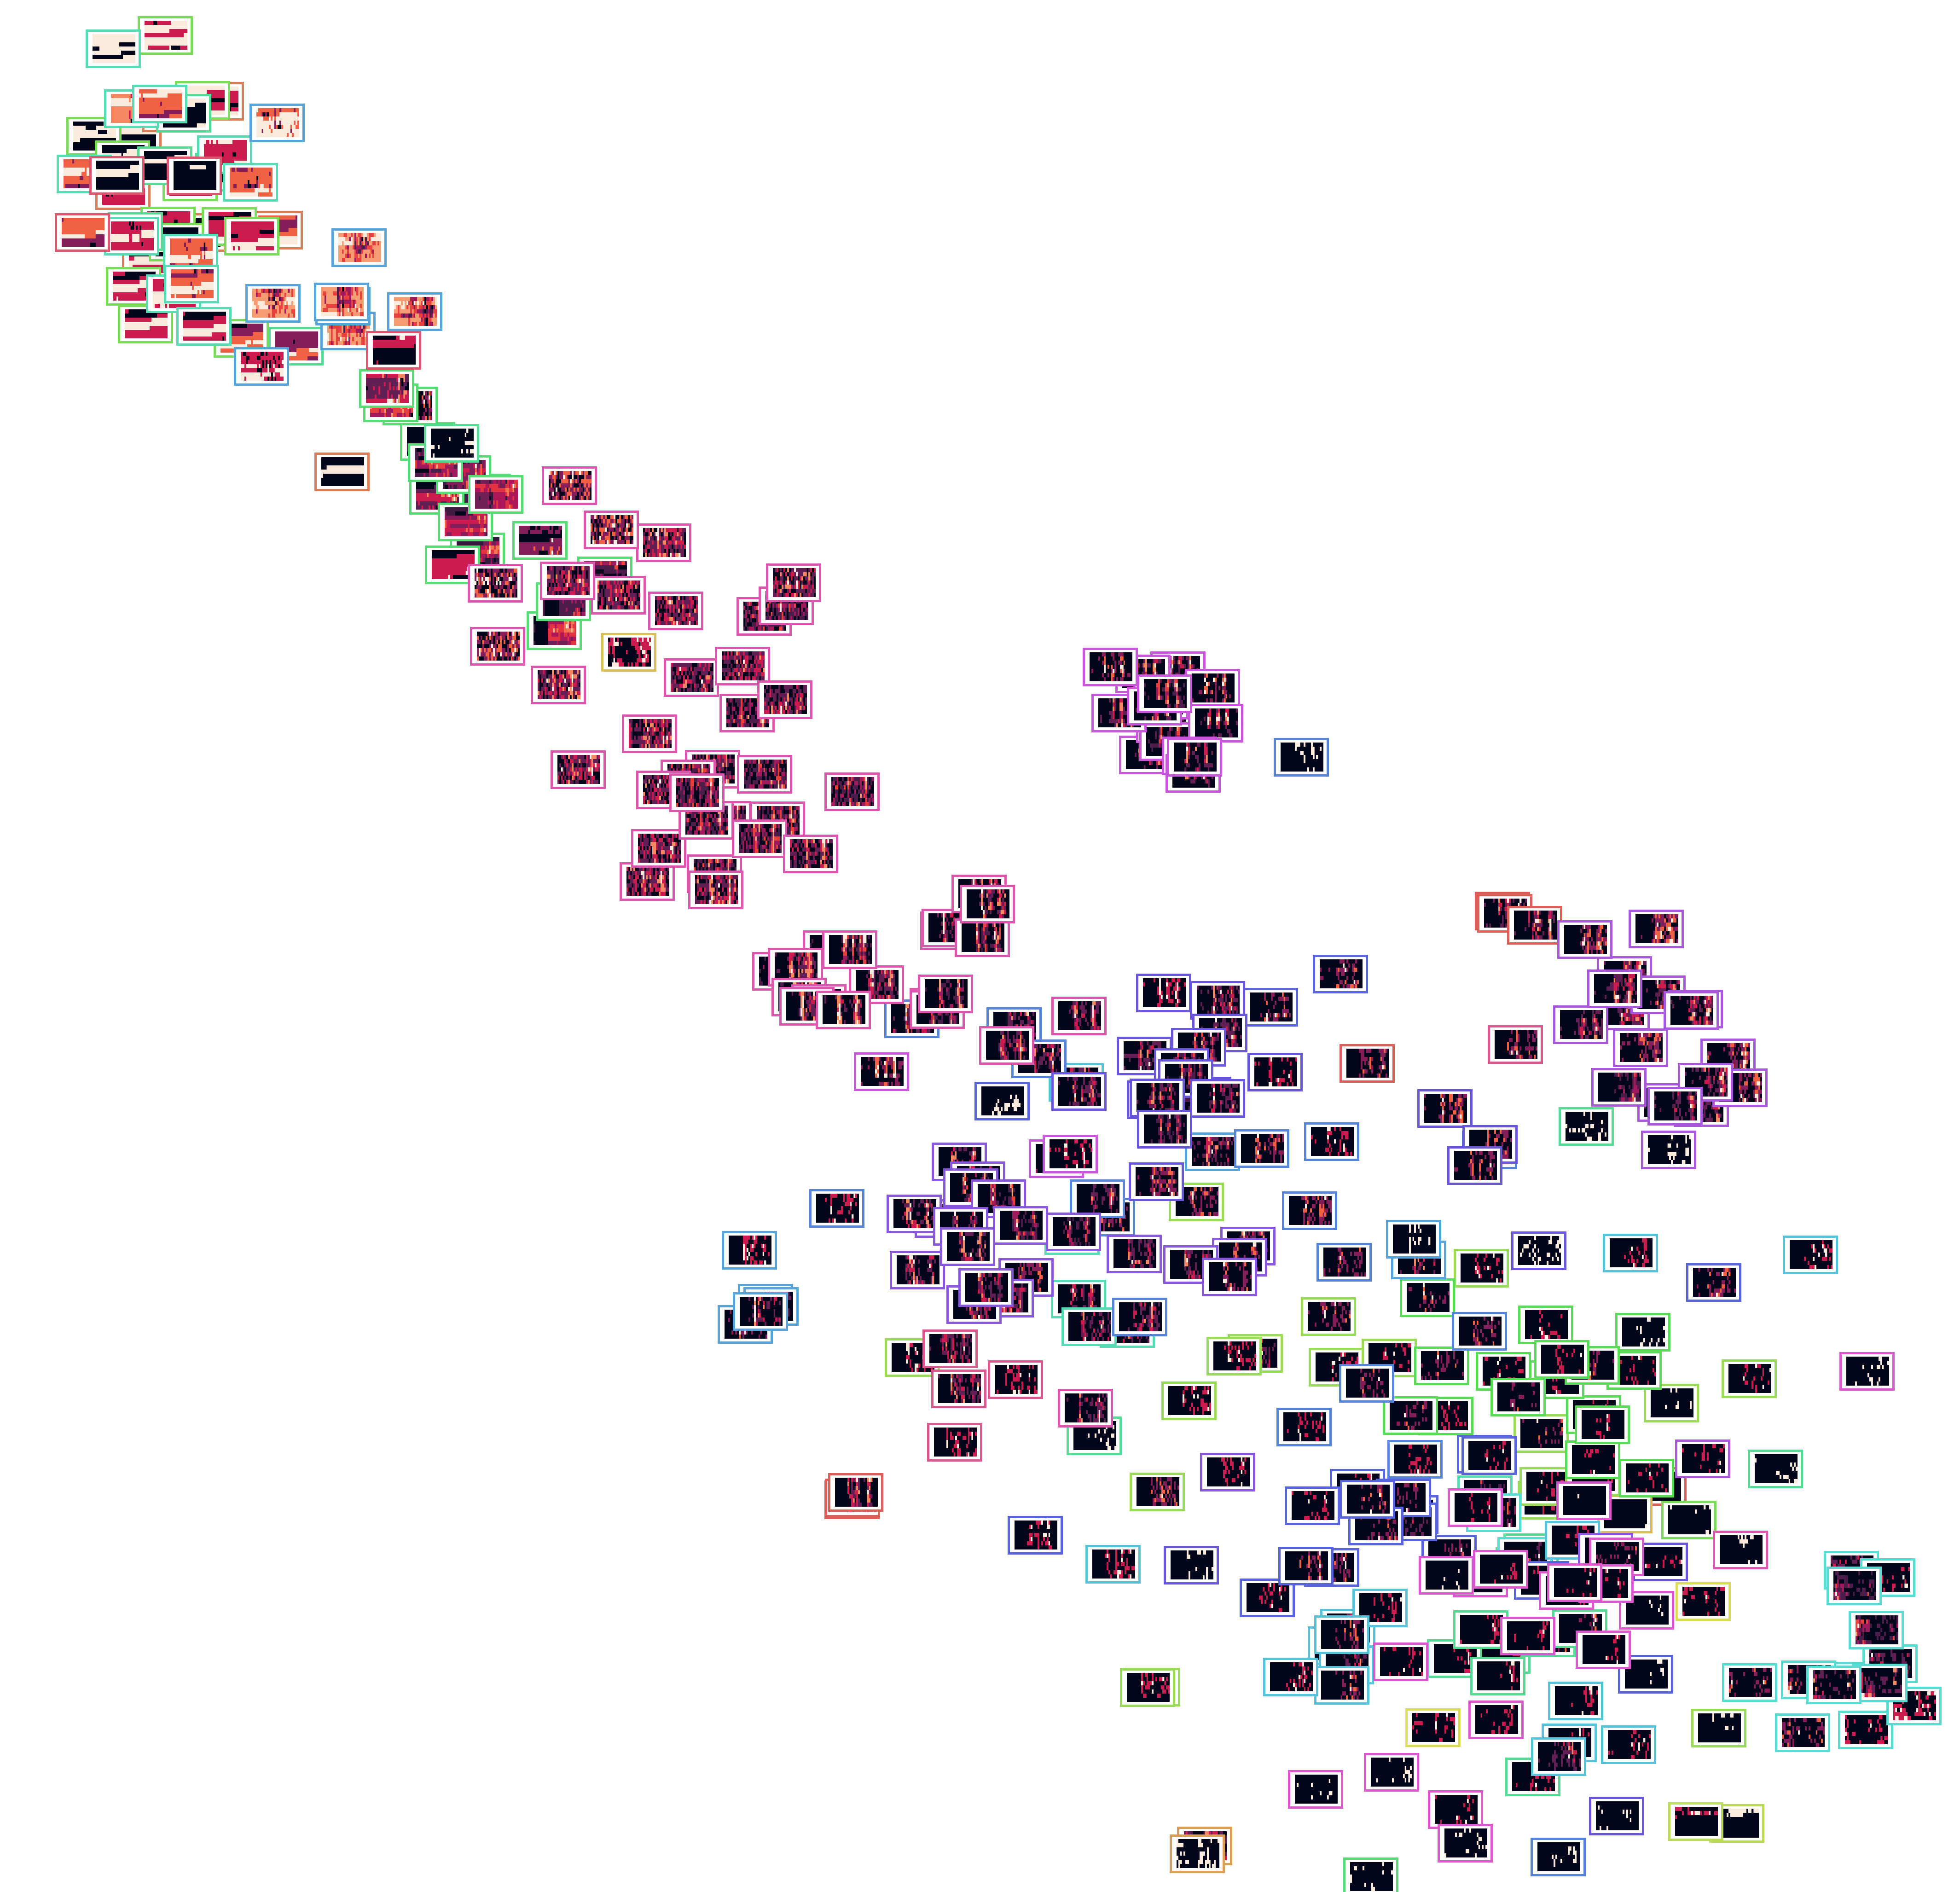
\includegraphics[width=.9\textwidth]{Figures/TSNE/TSNE_per_appliance/all/img_scatter_allmicrowave.png}
% 	\label{fig:tsne_pa_img_scatter_all_microwave}
% \end{figure}

The last per-appliance example is television presented in Figure \ref{fig:tsne_pa_scatter_all_tv}. 
Television was chosen since it is the most commonly occurring appliance.
Interestingly enough, televisions form nice clusters with a few outliers.
Clusters are separated but close together, this could mean that usage patterns across buildings are unique
but not that different from one another. 
The LPs in some clusters are also close to each other, which could also indicate 
a higher routine.

\begin{figure}[H]
	\centering
	\caption{Projection of TV LPs for various buildings}
	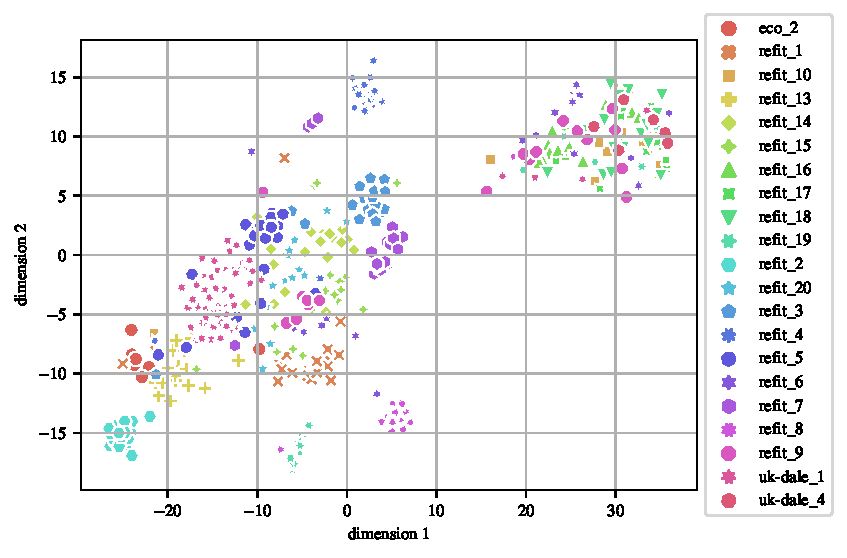
\includegraphics[]{Figures/TSNE/TSNE_per_appliance/scatter_refit_television.pdf}
	\label{fig:tsne_pa_scatter_all_tv}
	\par
	\par\footnotesize{Full resolution figure: \url{https://github.com/jenkoj/msc/tree/main/Figures/TSNE/TSNE_per_appliance/scatter_refit_television.pdf}}
\end{figure}

The images in Figure \ref{fig:tsne_pa_img_scatter_all_tv} prove the fact that outliers' consumption is a lot different.
Again the bright images could be the results of faulty appliances, faulty meters or simply odd behavior.
Figure \ref{fig:tsne_pa_img_scatter_all_tv} also enables us to see that TVs are primarily used 
in the evening hours. Outliers from the main cluster show slightly different behavior. One such 
example is the blue cluster (building REFIT 4), where appliances are mostly used in the morning hours. 
One other interesting observation can be made when looking at the purple cluster. This is the far low cluster for building REFIT 8.
Here, the TV is being consistently used every day in the early morning hours.
This is portrayed as a straight line.
There could be two possible explanations for this.
First is simply a high routine of a user, who turns on the TV every morning to listen to the news.
The other is that the TV updates itself every morning. This is probably not the case since updates do not occur on regular basis.
What is also interesting, is that the very same pattern can be observed in a few other buildings, one example being building REFIT 19.

\begin{figure}[H]
	\centering
	\caption{Projection of TV LPs for various buildings with actual samples.}
	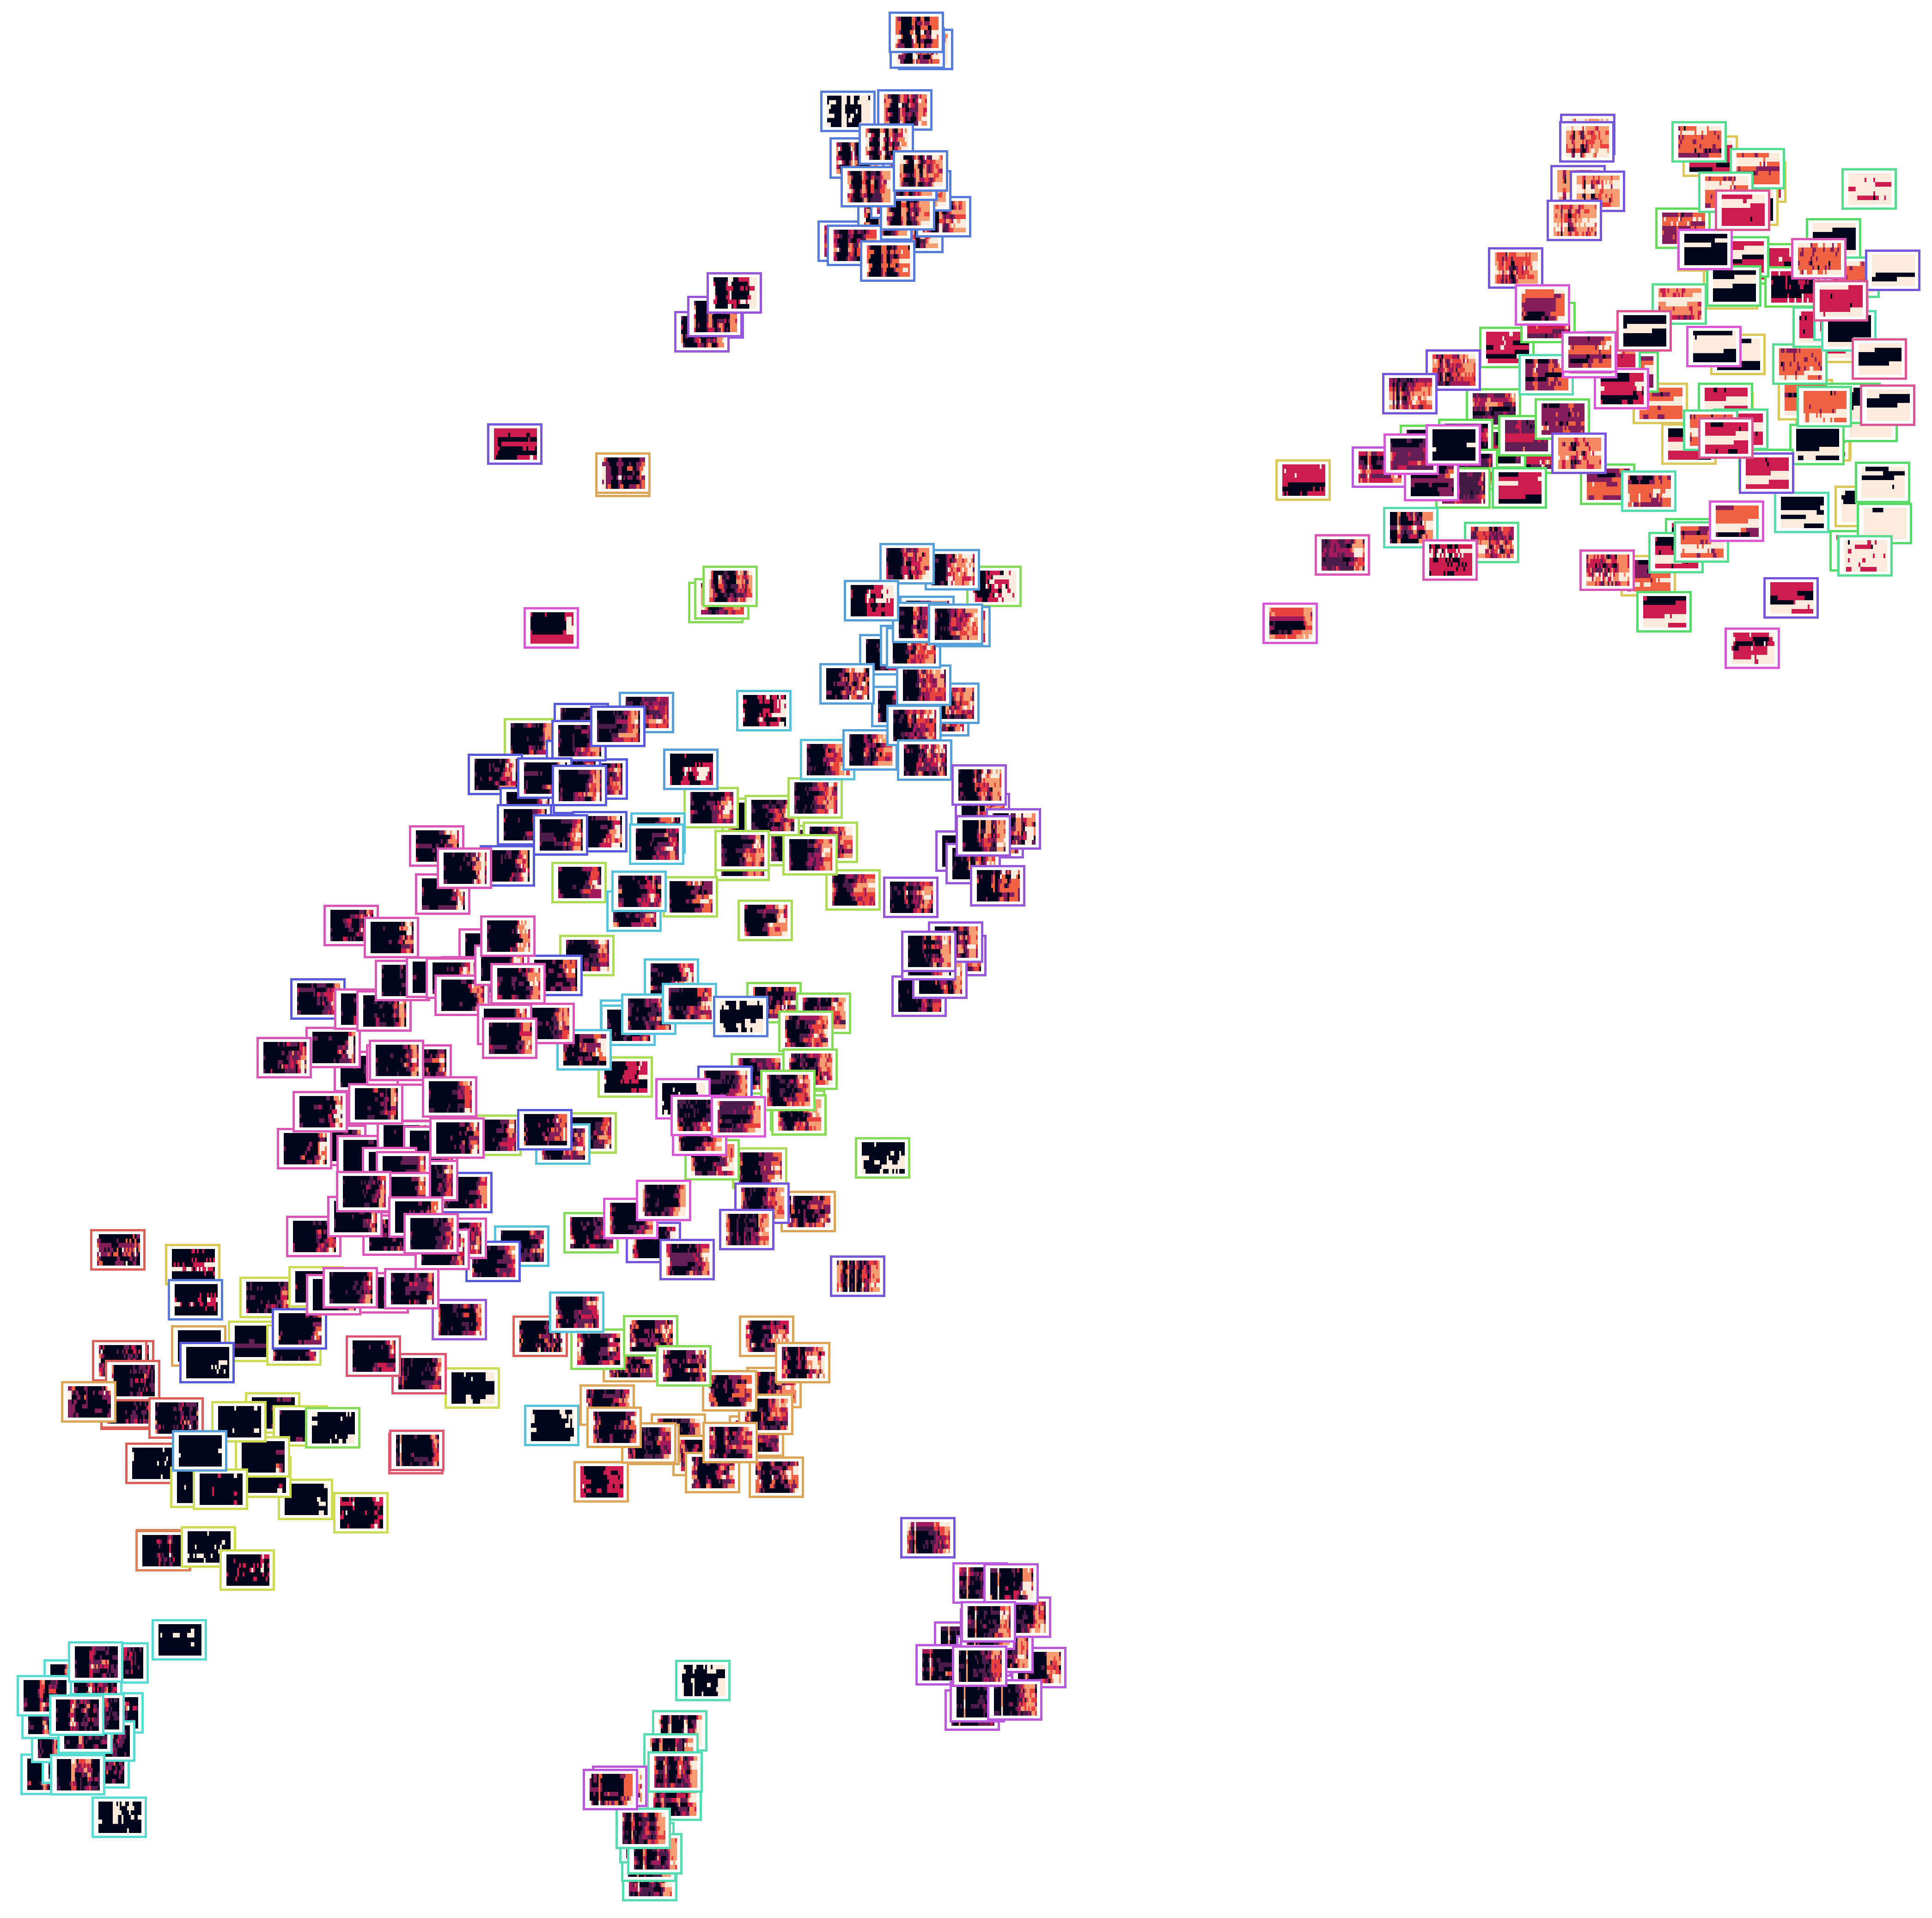
\includegraphics[width=.9\textwidth]{Figures/TSNE/TSNE_per_appliance/img_scatter_refit_television.png}
	\label{fig:tsne_pa_img_scatter_all_tv}
	\par
	\par\footnotesize{Full resolution figure: \url{https://github.com/jenkoj/msc/tree/main/Figures/TSNE/TSNE_per_appliance/img_scatter_refit_television.png}}
\end{figure}

\subsubsection{Per-Appliance LPs - Comparing Appliances}

% Figure \ref{fig:tsne_papb_scatter_all} presents the general picture of where each appliance lays in comparison to the other.
% One obvious issue here is that there are too many appliances, and it is impossible to comprehend the plot.

% \begin{figure}[H]
% 	\centering
% 	\caption{Projection of per-appliance LPs}
% 	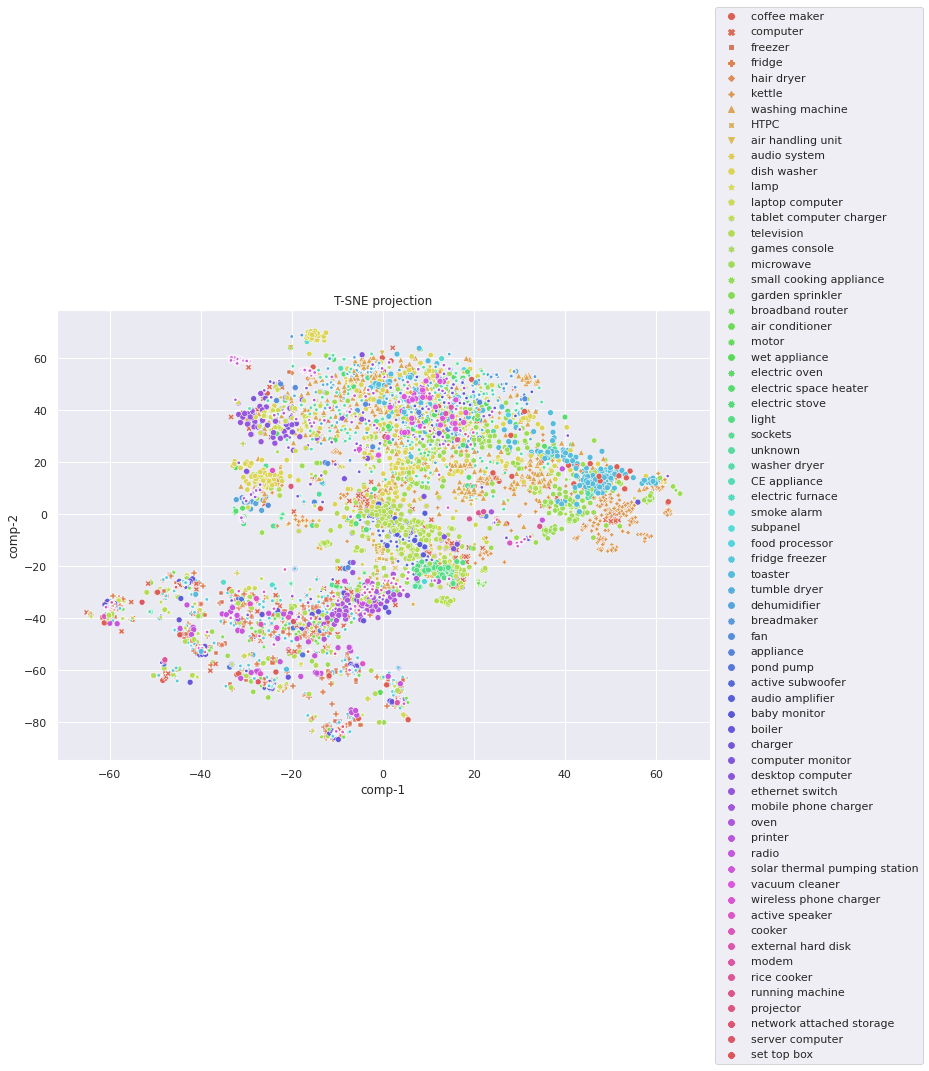
\includegraphics[width=1.2\textwidth]{Figures/TSNE/TSNE_results/all/scatter_all_all_lgimgs.png}
% 	\label{fig:tsne_papb_scatter_all}
% \end{figure}

% The same goes for image presentation in Figure \ref{fig:tsne_papb_img_scatter_all}. 
% We can see, that most active appliances are the ones in the bottom left,
% by moving to the upper right part of the corner, we can see less activity.
% Less activity does not necessarily mean that LPs contain less information about user behavior.

% \begin{figure}[H]
% 	\centering
% 	\caption{Projection of per-appliance LPs with actual samples}
% 	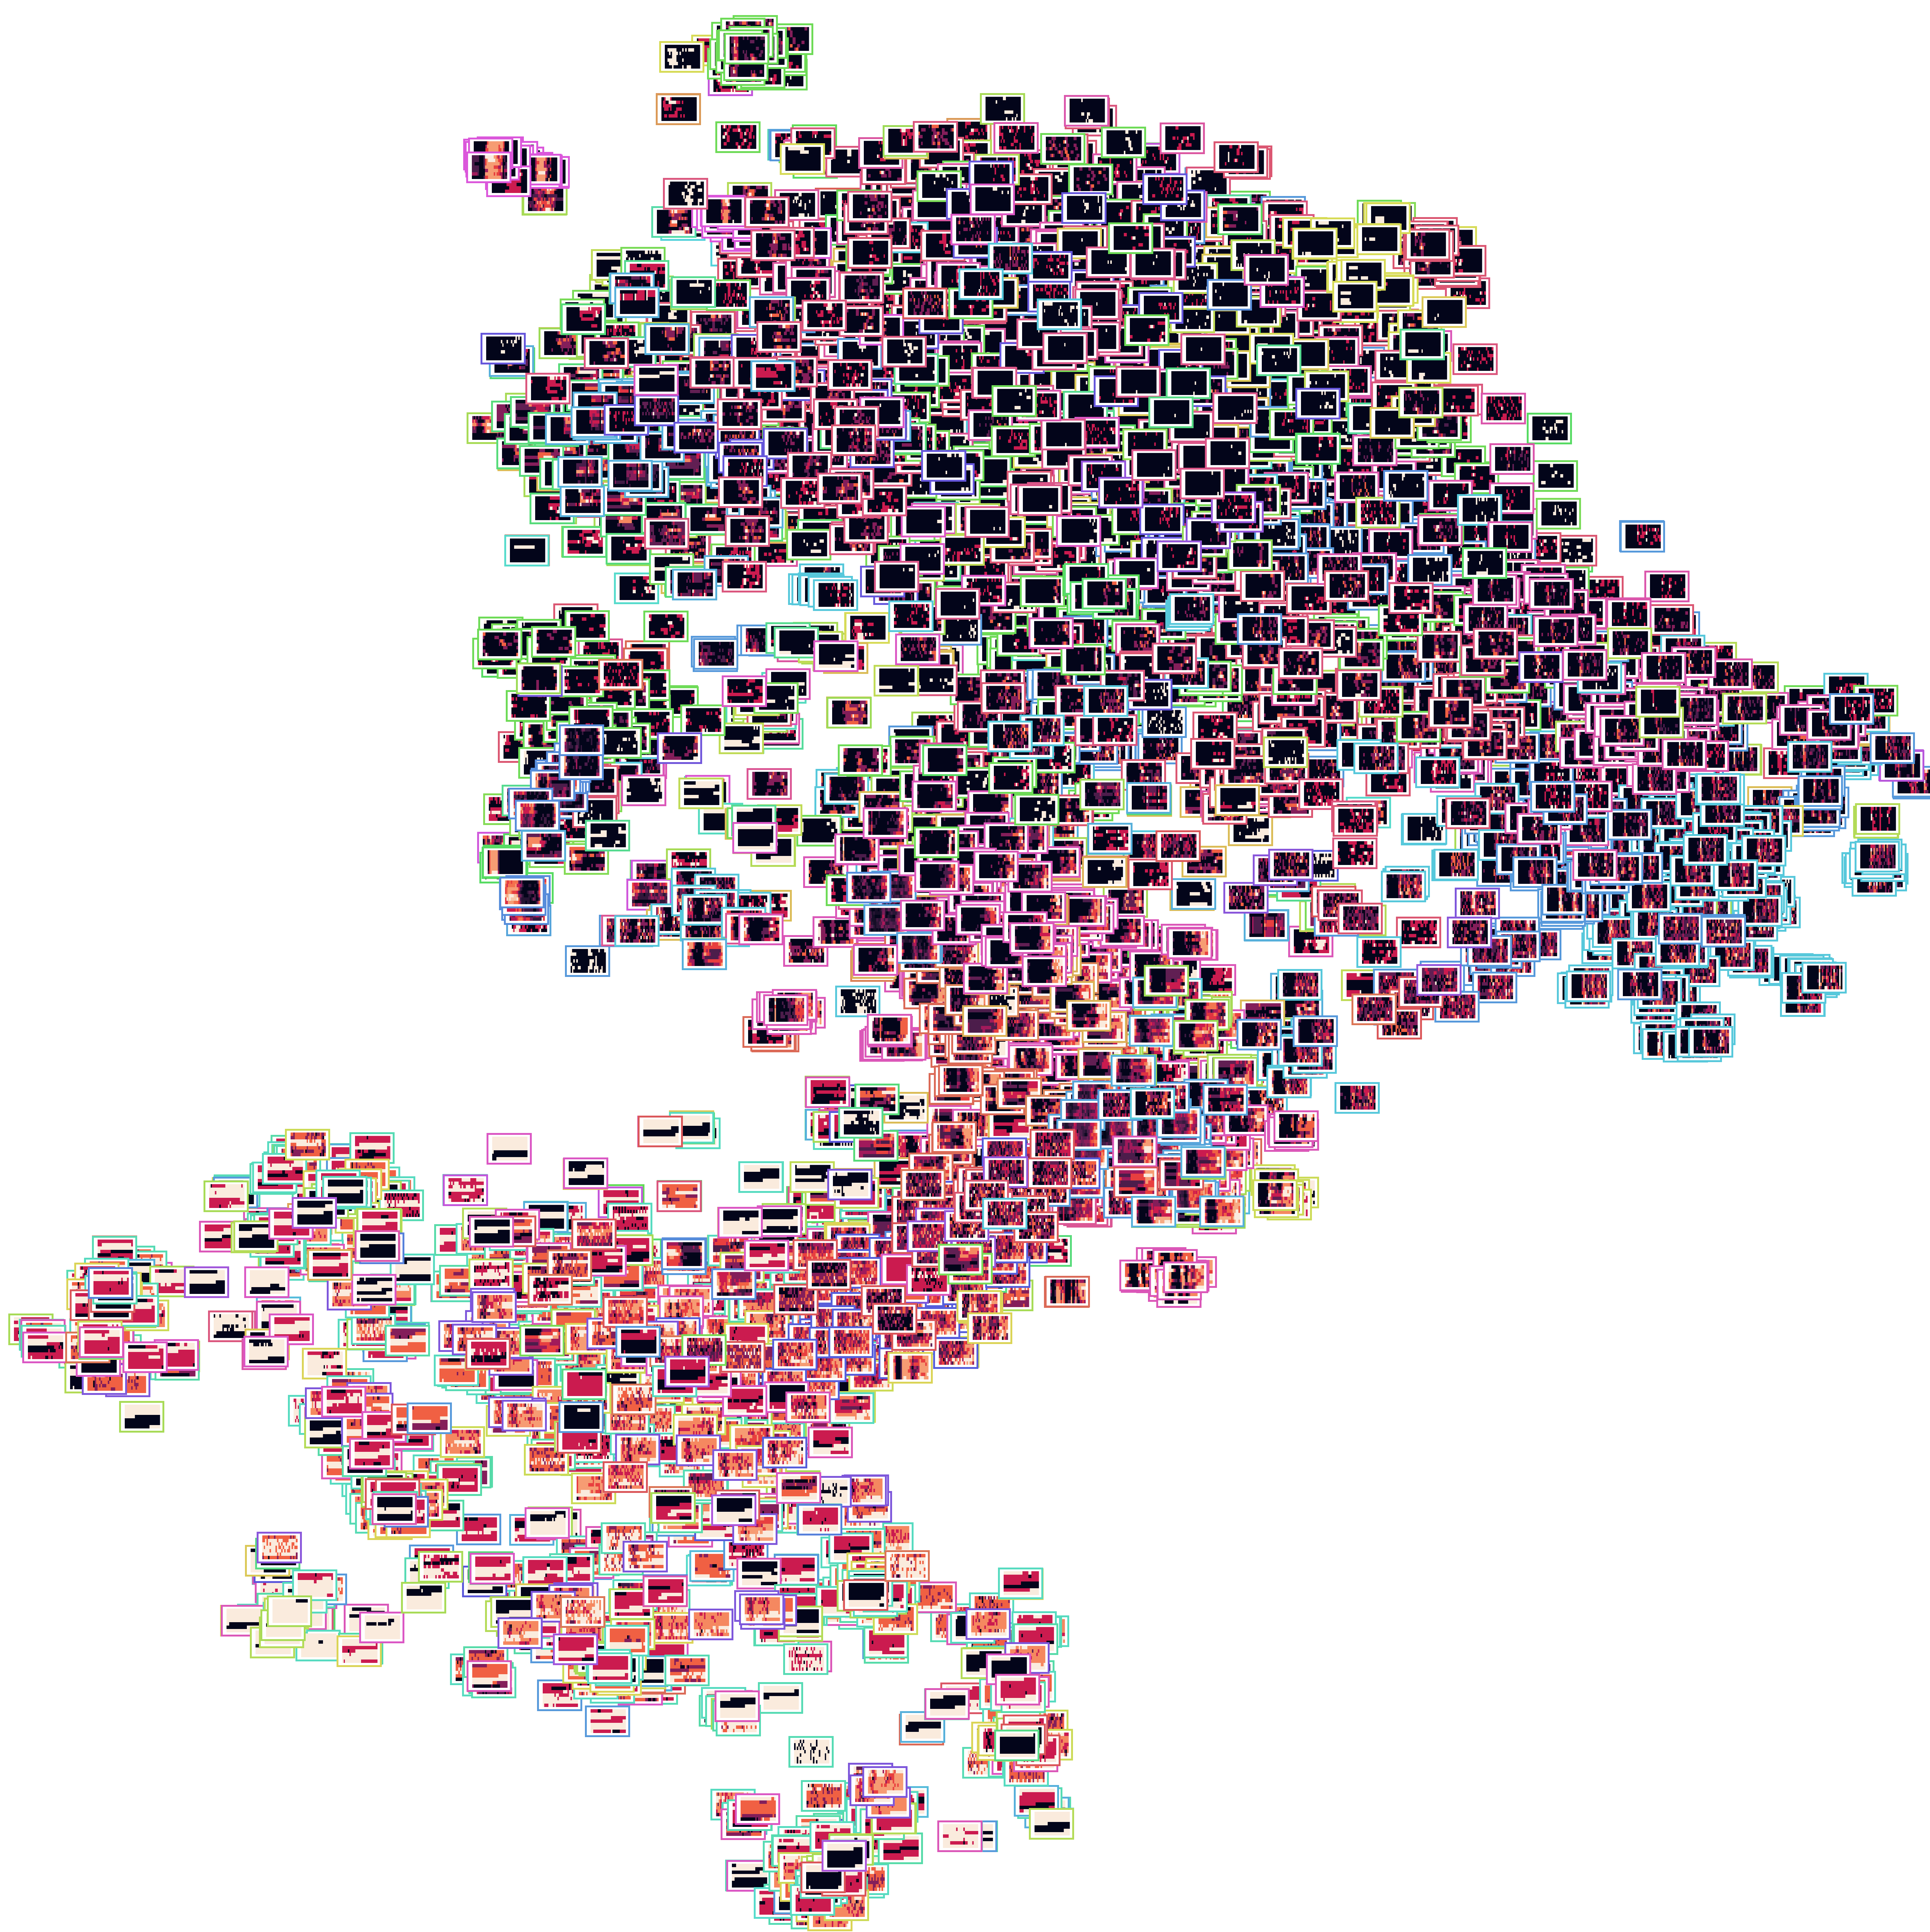
\includegraphics[width=.9\textwidth]{Figures/TSNE/TSNE_results/all/img_scatter_allall_lgimgs.png}
% 	\label{fig:tsne_papb_img_scatter_all}
% \end{figure}

To get a general idea of where each appliance group lies,
let's filter out all appliances that have less than 150 samples.
Applying this filter yields Figure \ref{fig:tsne_papb_scatter_all_reduced}.

\begin{figure}[H]
	\centering
	\caption{Projection of filtered per-appliance LPs}
	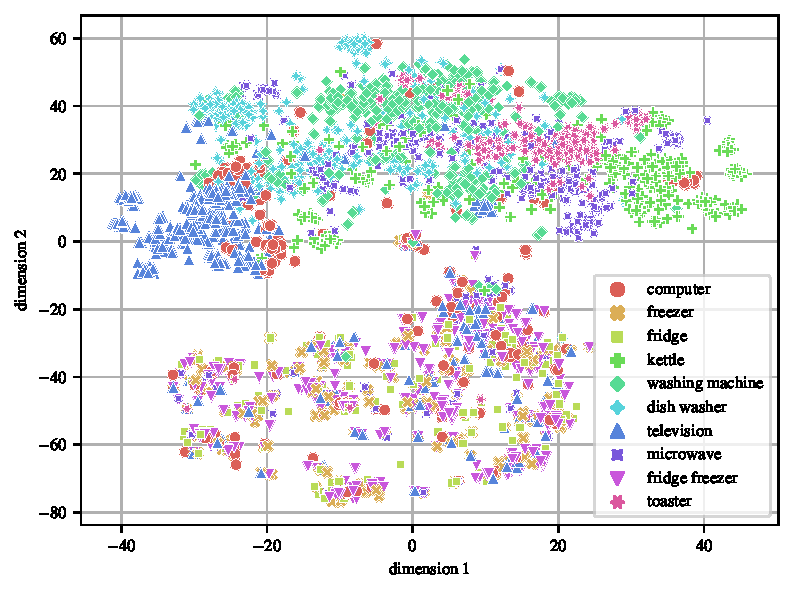
\includegraphics[]{Figures/TSNE/TSNE_PHPA/phpa_reduced_15.pdf}
	\label{fig:tsne_papb_scatter_all_reduced}
	\par
	\par\footnotesize{Full resolution figure: \url{https://github.com/jenkoj/msc/tree/main/Figures/TSNE/TSNE_PHPA/phpa_reduced_15.pdf}}
\end{figure}

Figure \ref{fig:tsne_papb_scatter_all_reduced} shows how these 10 appliances are connected in high dimensional space.
Kettles, microwaves and toasters are quite similar when it comes to usage patterns.
They are operated for a short amount of time and are usually used in users' routines in the morning or evening.
These appliances are located in the upper left part of the plot.

The second group of appliances that are quite near each other is white
goods (without fridges) such as washing machines, dishwashers, dryers etc.
Let's say that they are white goods with a program. 
This group of appliances is located in the upper right part of the plot.

The third group of appliances is white goods with a compressor.
They are usually not affected by human interaction and are therefore harder to cluster.
They are located in the lower part of the plot.

The final group of appliances is televisions and computers. They lie 
on a bridge between the fridges and other groups. 

% \begin{figure}[H]
% 	\centering
% 	\caption{Projection of filtered per-appliance LPs with actual samples}
% 	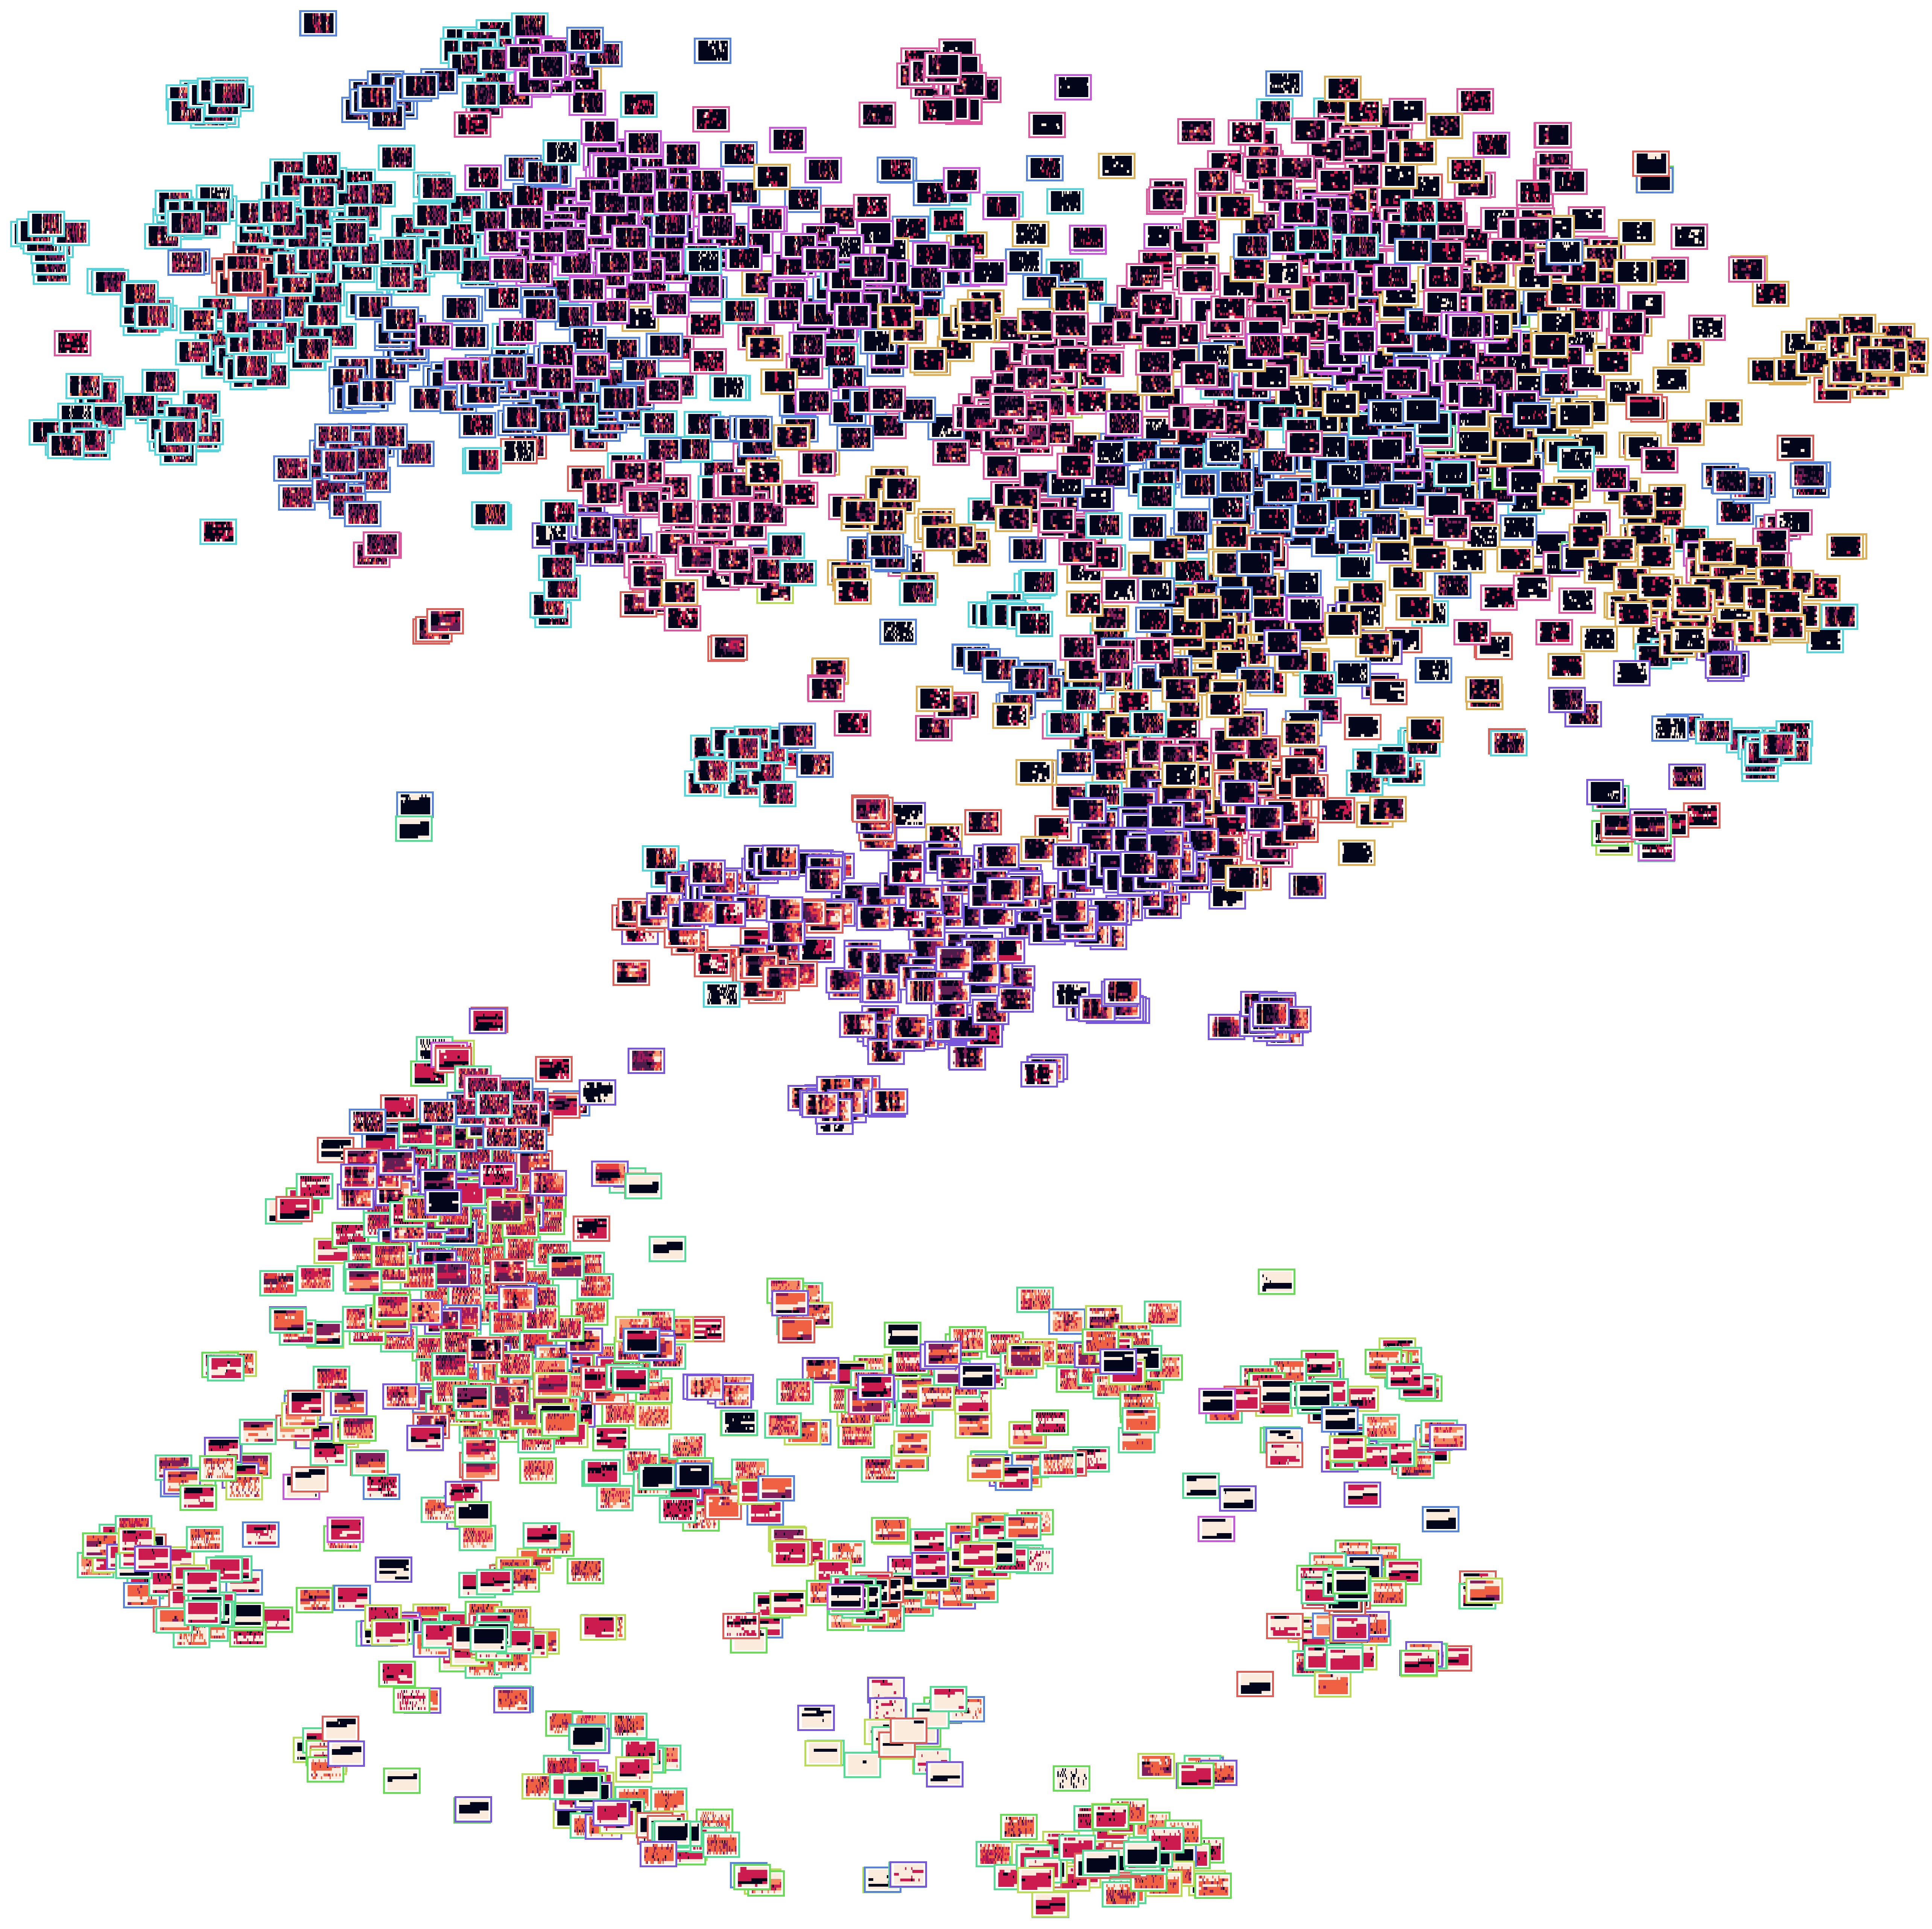
\includegraphics[width=.9\textwidth]{Figures/TSNE/TSNE_results/all/img_scatter_allall_reduced_max.png}
% 	\label{fig:tsne_papb_img_scatter_all_reduced}
% \end{figure}

% Even though the set of LPs is different due to filtering,
% the Figure \ref{fig:tsne_papb_img_scatter_all_reduced},
% retains a similar structure to the previous Figure \ref{fig:tsne_papb_scatter_all_reduced}. 

Knowing that a pattern exists, we can use the newly found group to define new appliance groups.
The following 8 groups will be defined
\begin{itemize}
    \item Kitchen appliances - toasters, ovens, microwaves, etc.
    \item Fridges and freezers  - contains fridges, freezers and fridge freezers or white goods with a compressor
    \item White goods - washers, dryers, dishwashers i.e. white goods with a program
    \item heating and cooling - Electric radiators, dehumidifiers and HVACs
    \item leisure -  Living room appliances such as TVs, games consoles, audio amps, HTPCs, etc.
    \item home office - Computer, laptops, printers, network equipment, chargers, etc.
    \item lightning - lights and lamps
    \item Others - unknown and unlabeled appliances
\end{itemize}

Applying these groups yields Figure \ref{fig:tsne_papb_scatter_all_groups}.
The new plot shows how, although appliances could be used by a different
user, maybe even by users in a different part of the EU or world,
they can be grouped in a high-dimensional space. 

\begin{figure}[H]
	\centering
	\caption{Projection of grouped per-appliance LPs}
	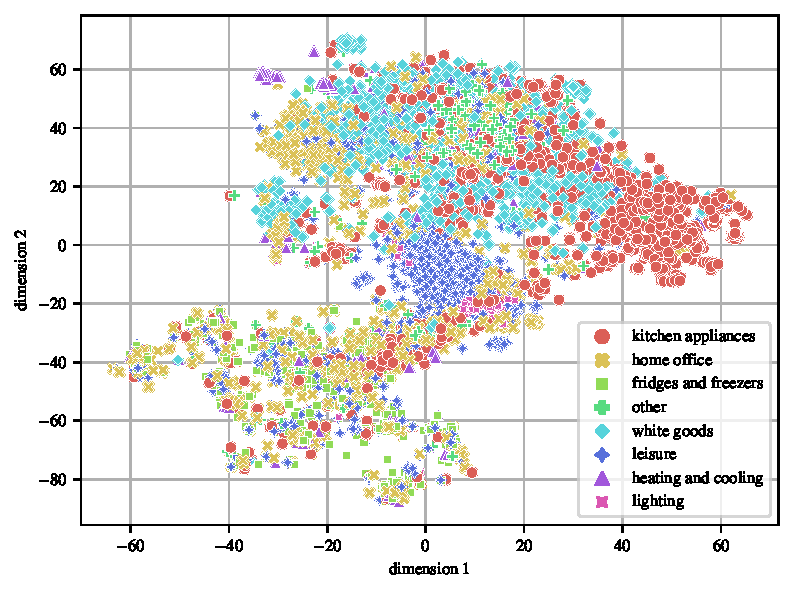
\includegraphics[]{Figures/TSNE/TSNE_PHPA/phpa_grouped_15.pdf}
	\label{fig:tsne_papb_scatter_all_groups}
	\par
	\par\footnotesize{Full resolution figure: \url{https://github.com/jenkoj/msc/tree/main/Figures/TSNE/TSNE_PHPA/phpa_grouped_15.pdf}}
\end{figure} 

The Figure \ref{fig:tsne_papb_img_scatter_all_groups} below is the same as the first Figure \ref{fig:tsne_papb_img_scatter_all} in the subsection,
except it is easier to use color to see the appliance they present

\begin{figure}[H]  
	\centering
	\caption{Projection of grouped per-appliance LPs with actual samples}
	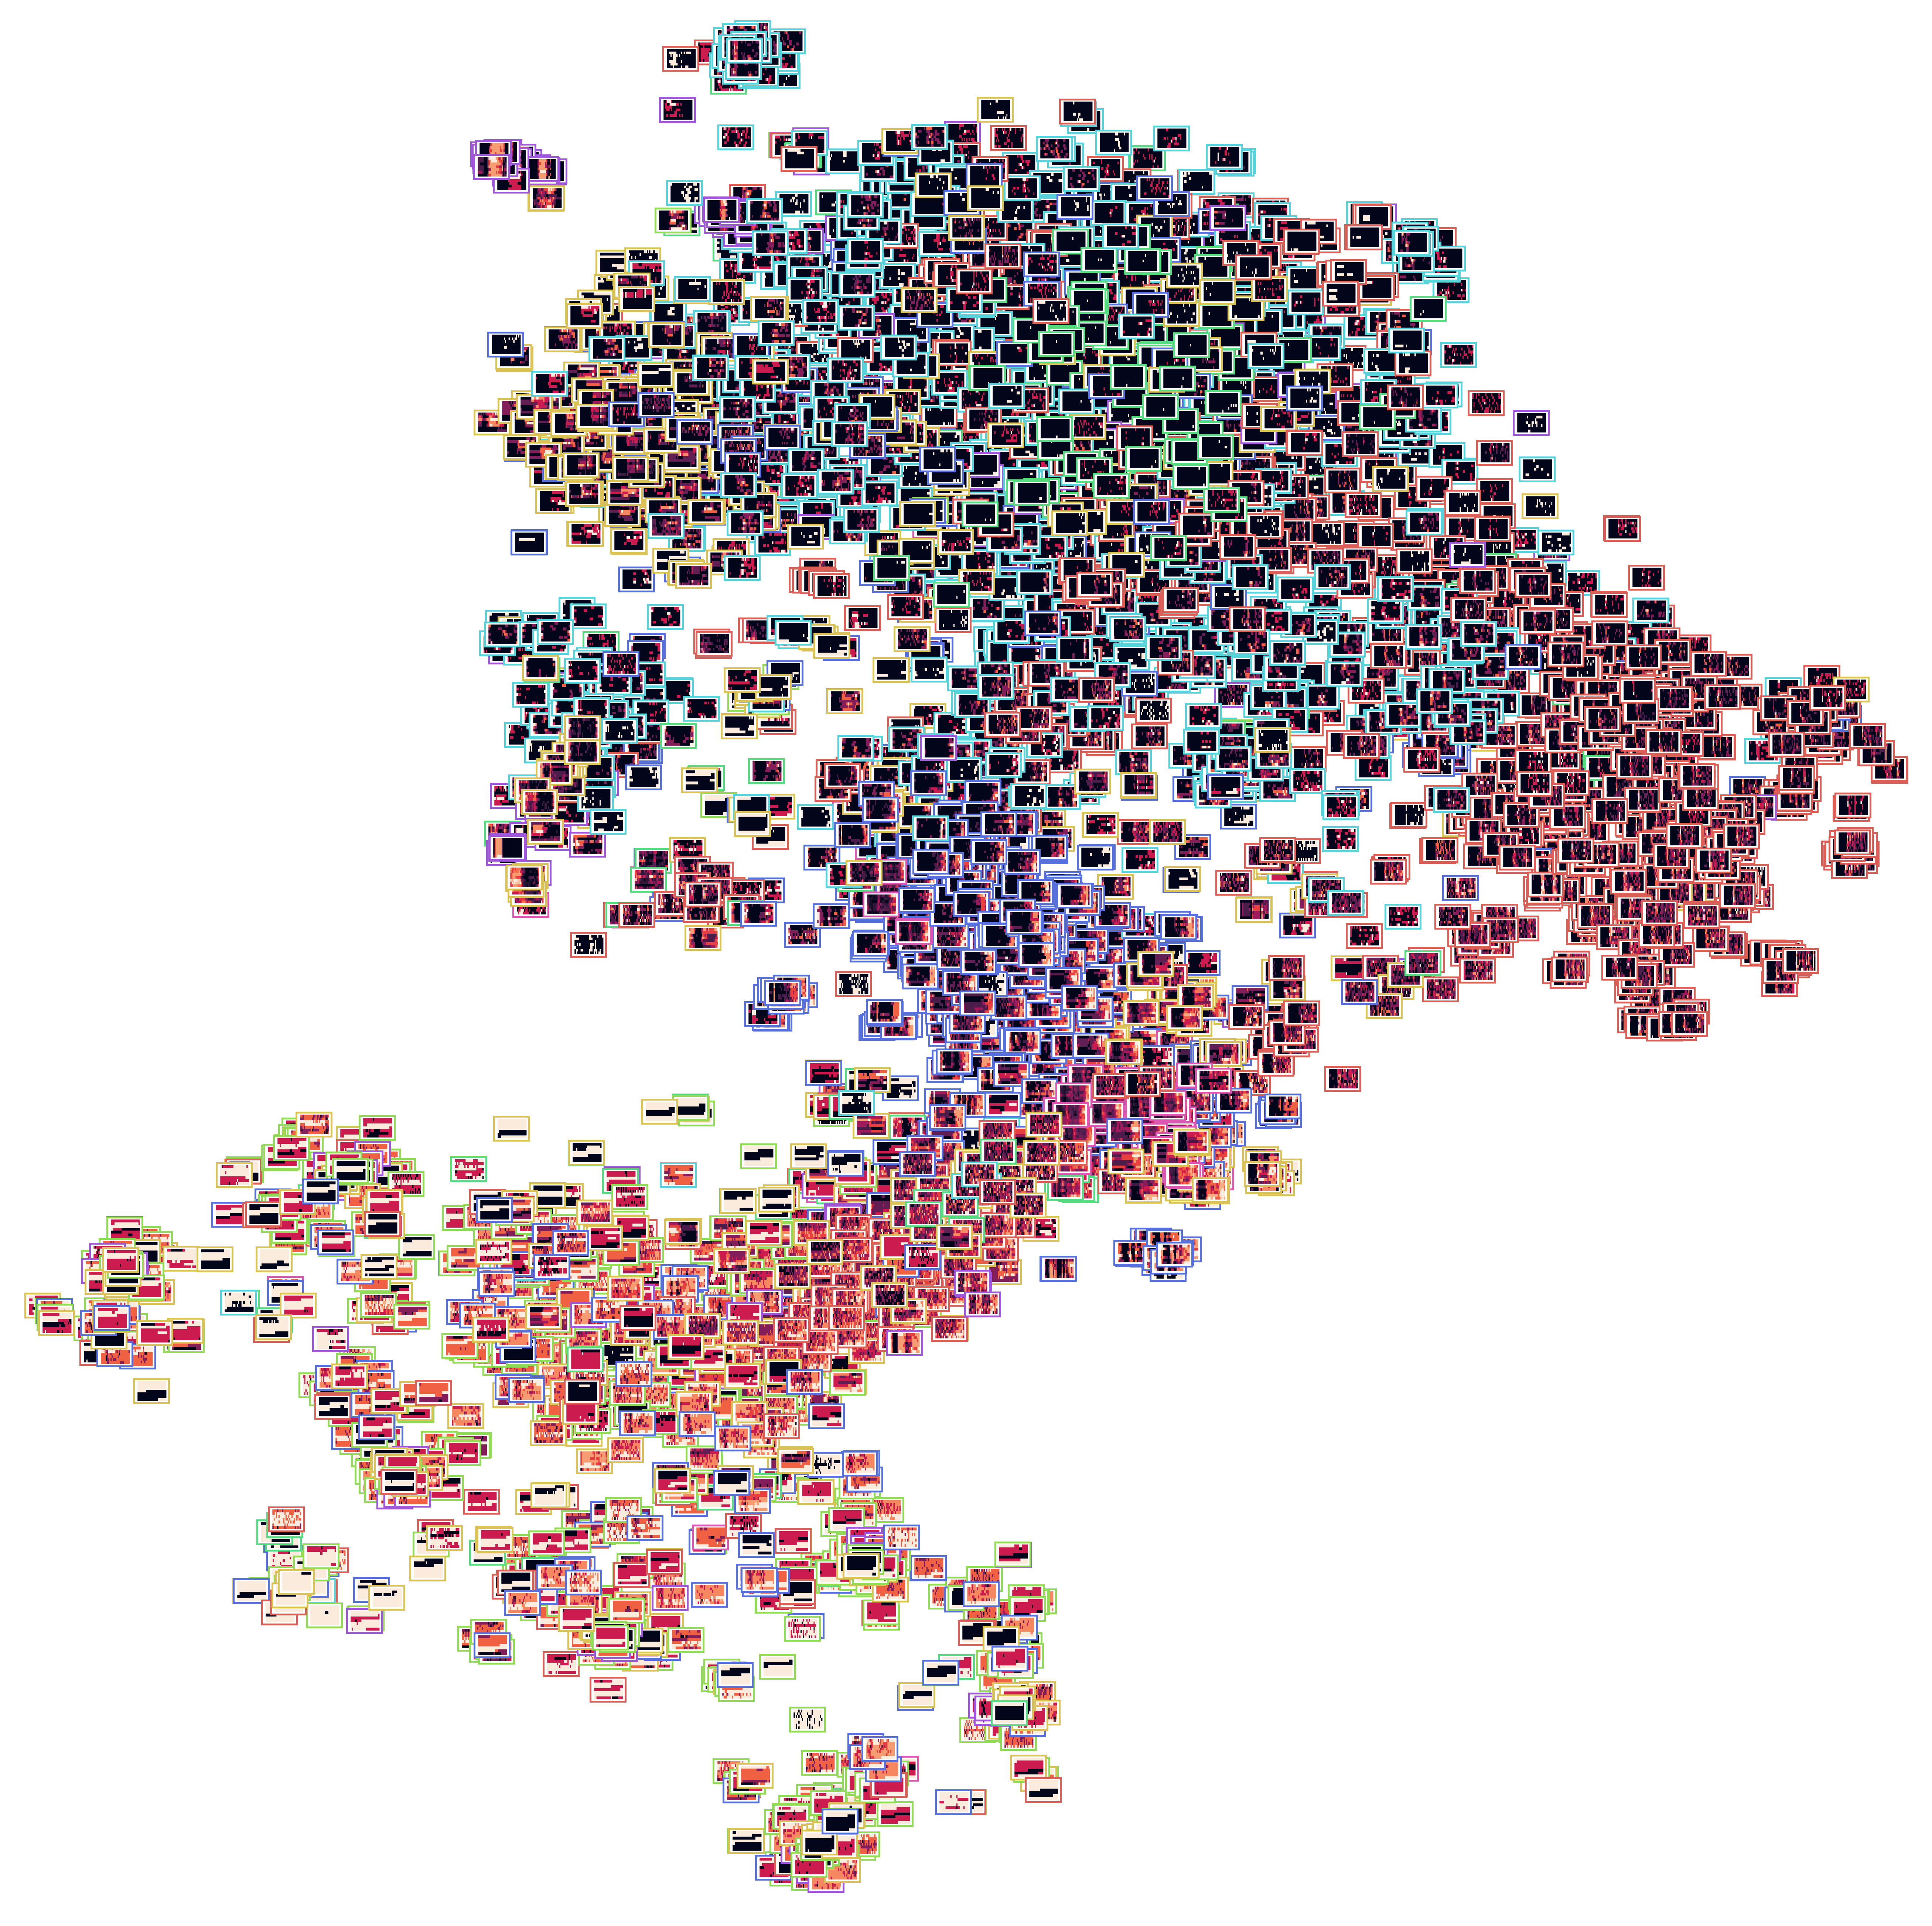
\includegraphics[width=.9\textwidth]{Figures/TSNE/TSNE_PHPA/img_scatter_all_all_groups.png}
	\label{fig:tsne_papb_img_scatter_all_groups}
	\par
	\par\footnotesize{Full resolution figure: \url{https://github.com/jenkoj/msc/tree/main/Figures/TSNE/TSNE_PHPA/img_scatter_all_all_groups.png}}
\end{figure}

To better emphasize the details from Figure \ref{fig:tsne_papb_img_scatter_all_groups} and \ref{fig:tsne_papb_scatter_all_groups} we present zoomed-in areas of key locations with Figure \ref{fig:t-sne_zoomed}.
\begin{figure}[H] 
	\centering
	\caption{Projection of grouped per-appliance LPs with actual samples}
	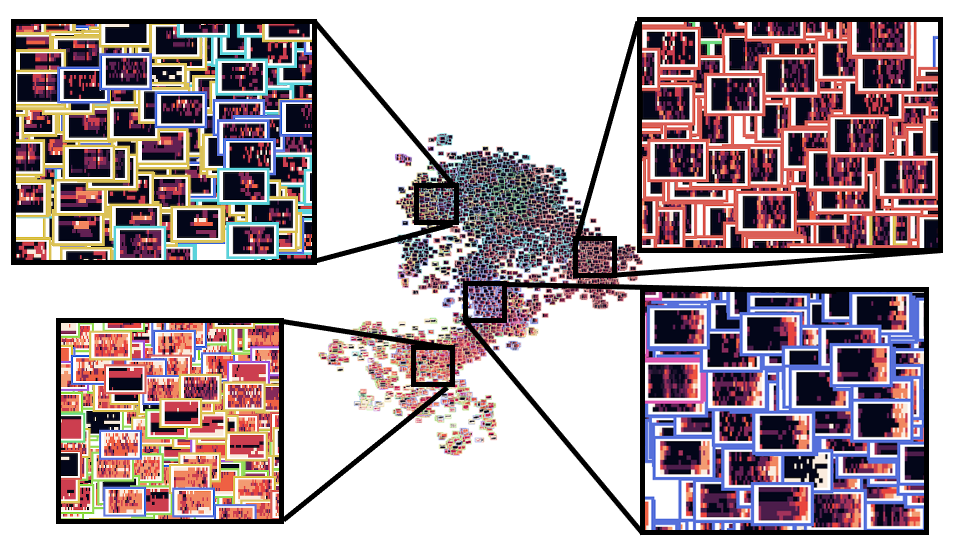
\includegraphics[width=.9\textwidth]{Figures/TSNE/TSNE_PHPA/t-sne_zoomed.png}
	\label{fig:t-sne_zoomed}
	\par
	\par\footnotesize{Full resolution figure: \url{https://github.com/jenkoj/msc/tree/main/Figures/TSNE/TSNE_PHPA/t-sne_zoomed.png}}
\end{figure}

% One issue that causes the t-SNE algorithm an issue is low entropy data or 
% in other words, images that are almost completely dark or white, due to various faults in appliances or measurements.

% If we calculate the entropy for each image and set a threshold, it is possible to filter out these samples. 
% By setting an entropy threshold of 0.5, we filter out around 5 \% of all samples. 

% \begin{figure}[H]
% 	\centering
% 	\caption{Projection of entropy filtered per-appliance LPs}
% 	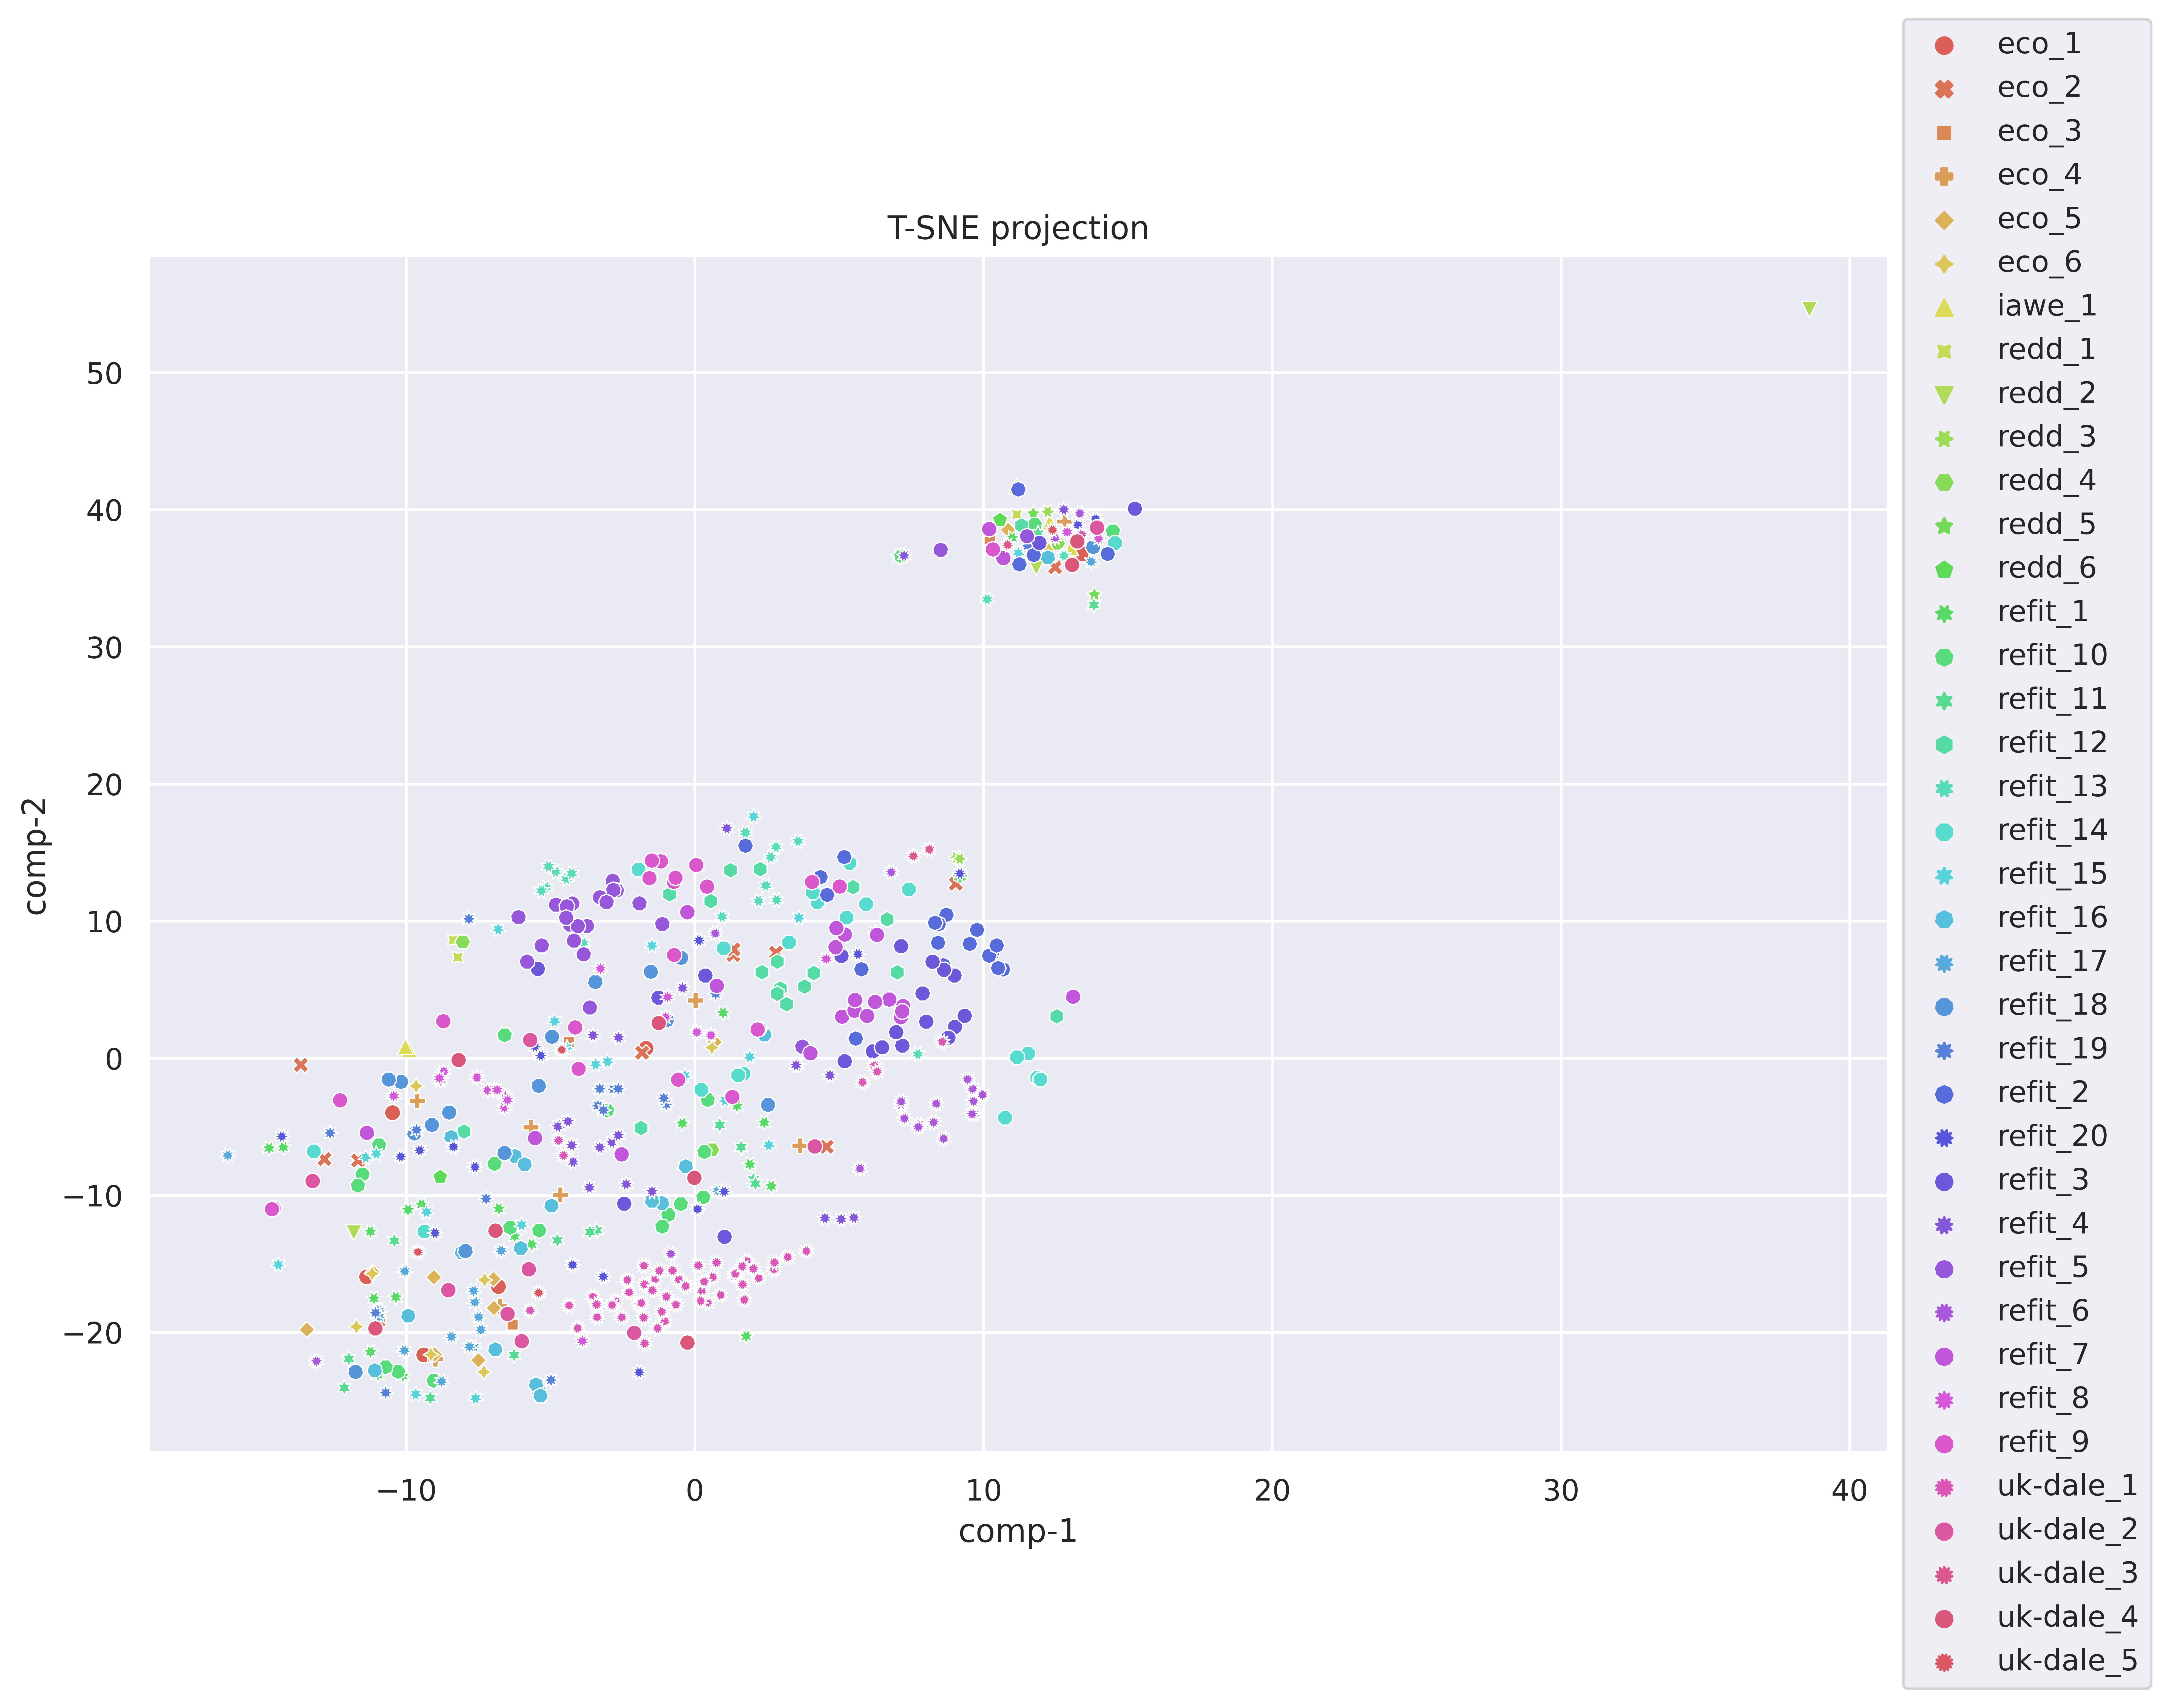
\includegraphics[width=.8\textwidth]{Figures/TSNE/TSNE_results_entropy/all/scatter_all_all.png}
% 	\label{fig:tsne_papb_scatter_ent_all_groups}
% \end{figure}

% Again, we can apply appliance grouping and get nicely formed clusters, such as can be seen in Figure \ref{fig:tsne_papb_img_scatter_ent_all_groups}.

% \begin{figure}[H]
% 	\centering
% 	\caption{Projection of entropy filtered per-appliance LPs with actual samples}
% 	\includegraphics[width=.8\textwidth]{Figures/TSNE/TSNE_results_entropy/all/scatter_all_all_groups.png}
% 	\label{fig:tsne_papb_img_scatter_ent_all_groups}
% \end{figure}


% \subsubsection{Comparing Appliances in a Building}

% It is also possible to use per-appliance data to study
% individual buildings, and how each appliance is used.
% In this case, we have used building 8 from REFIT as an example.

% \begin{figure}[H]
% 	\centering
% 	\caption{Projection of per-appliance LPs in a single building}
% 	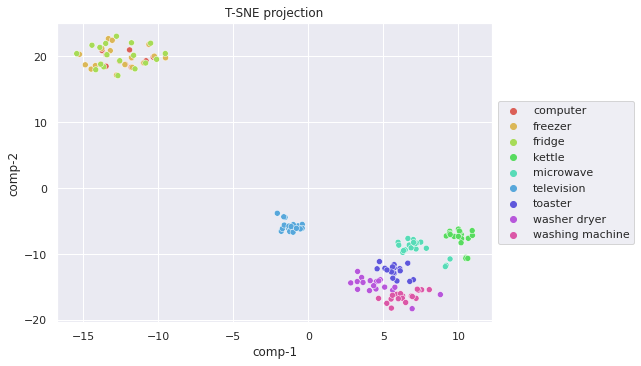
\includegraphics[width=.8\textwidth]{Figures/TSNE/TSNE_results/refit/scatter_refit_8.png}
% 	\label{fig:tsne_papb_scatter_ent_refit8}
% \end{figure}

% In general, the scattering is similar to before.
% Fridges and freezers are located opposite of white goods and kitchen appliances. 
% The television lies somewhere in between. 

% \begin{figure}[H]
% 	\centering
% 	\caption{Projection of per-appliance LPs in a single building with actual samples}
% 	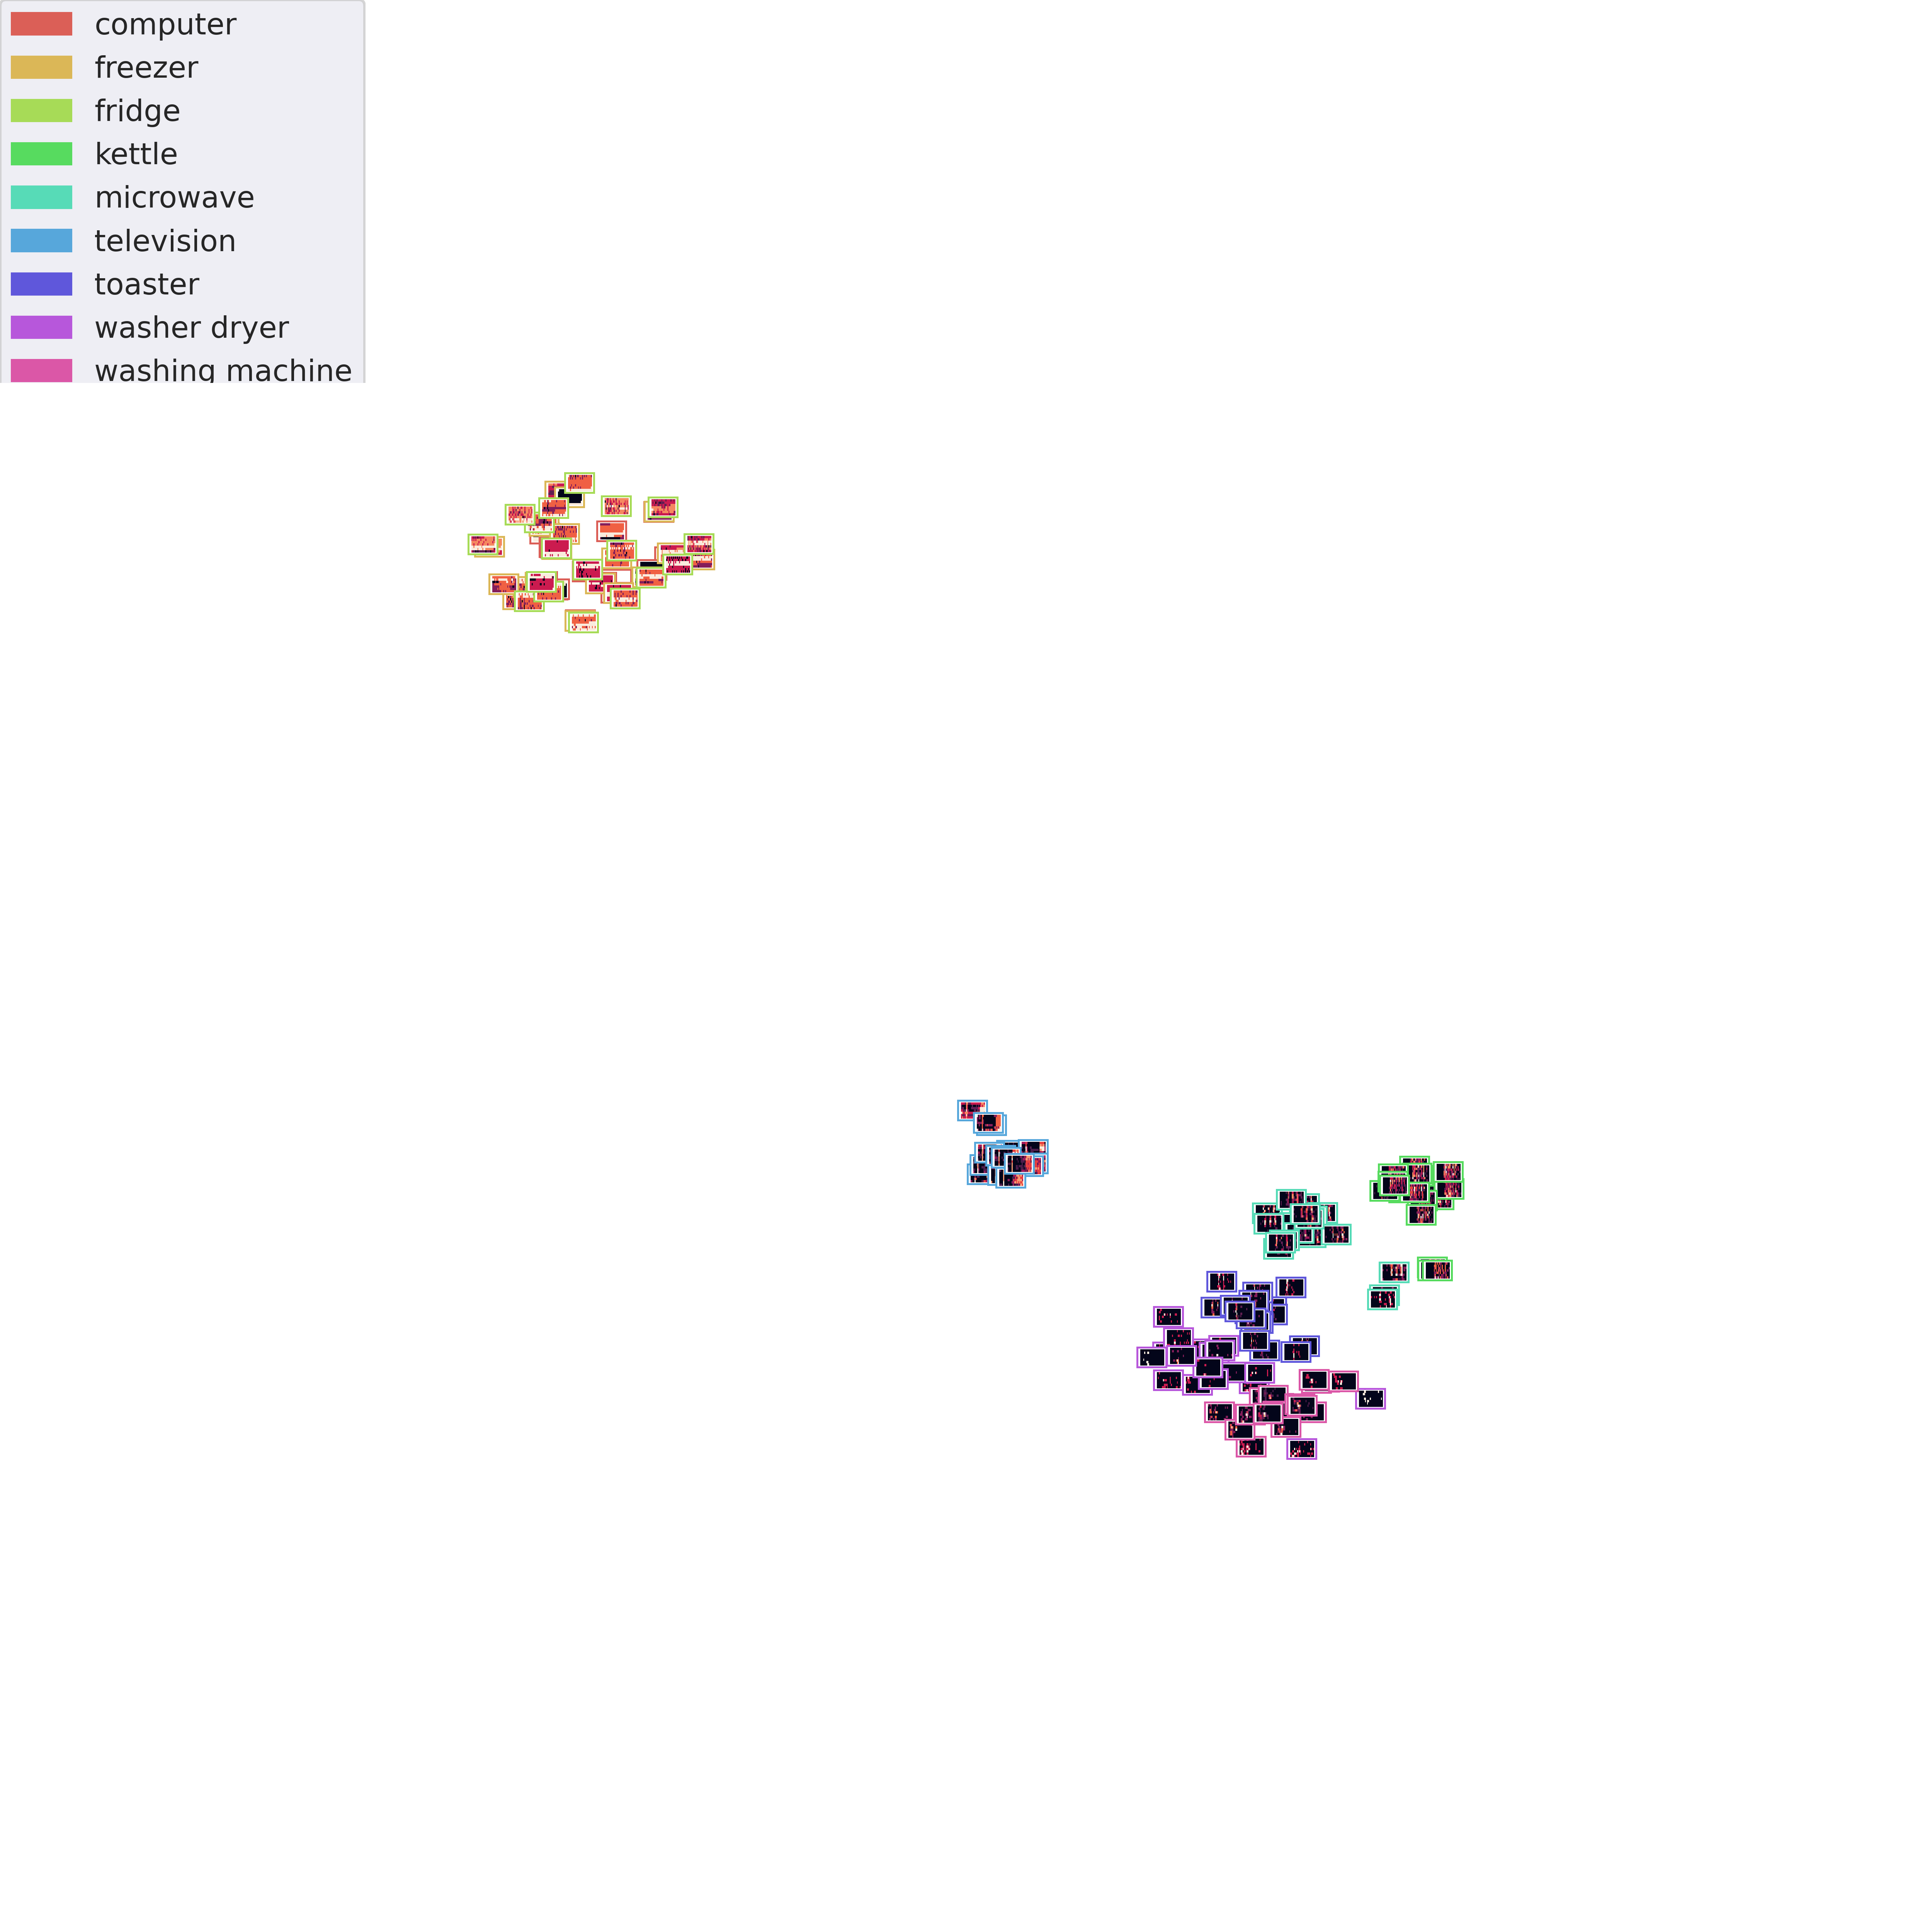
\includegraphics[width=.9\textwidth]{Figures/TSNE/TSNE_results/refit/img_scatter_refit8.png}
% 	\label{fig:tsne_papb_img_scatter_ent_refit8}
% \end{figure}

% Similar to before Figure \ref{fig:tsne_papb_img_scatter_ent_refit8} shows the fridge cluster as the most active,
% with the least interesting information. In the middle, we can again observe the TV that is mostly being used
% in the evening hours. The samples also point to the possibility of a high-user routine in the early morning hours.
% The high routine is portrayed as a straight line on the figures. 

% In this case, when observing white goods in pink and purple boxes, it is possible to see that this user primarily uses them during the night hours.
% This could point out that the user is making use of cheaper tariffs.

% One other interesting observation that can be made here is comparing kettles, microwaves and toasters.
% Usually, these appliances are used similarly and in similar parts of the day. 
% Here the toaster and microwave are being used periodically, but the kettle is being used throughout the day with no general pattern.
% It is self-obvious that some users have higher routines than others, but this observation
% would add that some users can have a higher routine for some appliances and lower for others, of the same type. 

\subsection{Per-Appliance Per-Building}

To study the usage by comparing all appliances between buildings,
we have to use one of the proposed LPs and in this case, this is a Bag of appliances.

\subsubsection{Bag of Appliances}

This LP is a combination of the LPs above,
except it offers a larger detail when observing groups of appliances.
Since we are using one dimension for appliances, we will use only the daily dimension.

To construct such a profile we need a universal way of constructing it.
This is done by measuring how many times each appliance occurs in the datasets,
then this list is sorted from most common to least common, and finally, the top 30 are selected.

The problem with such a comparison is, that it is best 
if all buildings would use the same appliances.
Since that is not the case, missing appliances are portrayed as always off. 

This is the main reason why we can see in Figure \ref{fig:tsne_boa_scatter_refit8} the clusters are separated quite a bit.
We can still see that some clusters are closer than others,
meaning they are more similar.  

\begin{figure}[H]
	\centering
	\caption{Projection of a bag of appliances LPs for various buildings}
	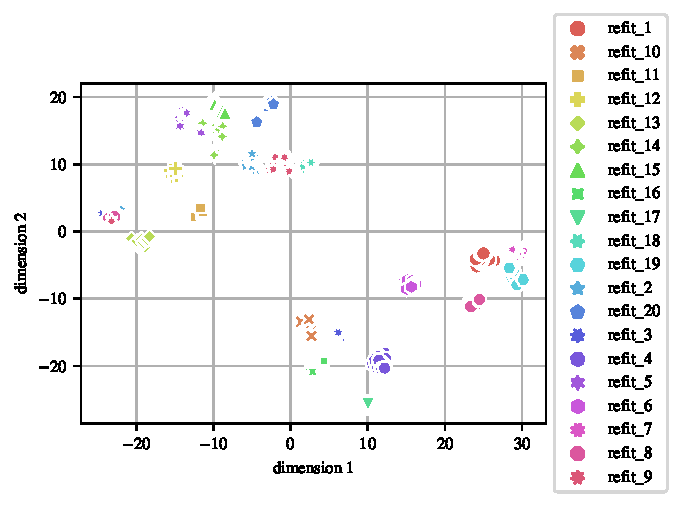
\includegraphics[]{Figures/TSNE/TSNE_BOA/scatter_refit_boa.pdf}
	\label{fig:tsne_boa_scatter_refit8}
	\par
	\par\footnotesize{Full resolution figure: \url{https://github.com/jenkoj/msc/tree/main/Figures/TSNE/TSNE_BOA/scatter_refit_boa.pdf}}
\end{figure} 

Figure \ref{fig:tsne_boa_img_scatter_refit8} shows that LPs are split 
between two poles. 
By observing the Figure it is possible to see that all the bottom clusters
have more than one active white good with a compressor (fridges and freezers), while
the top ones have only one. In general, the bottom buildings have more appliances,
with more activity than the top ones. 

\begin{figure}[H]
	\centering
	\caption{Projection of a bag of appliances LPs for various buildings with actual samples}
	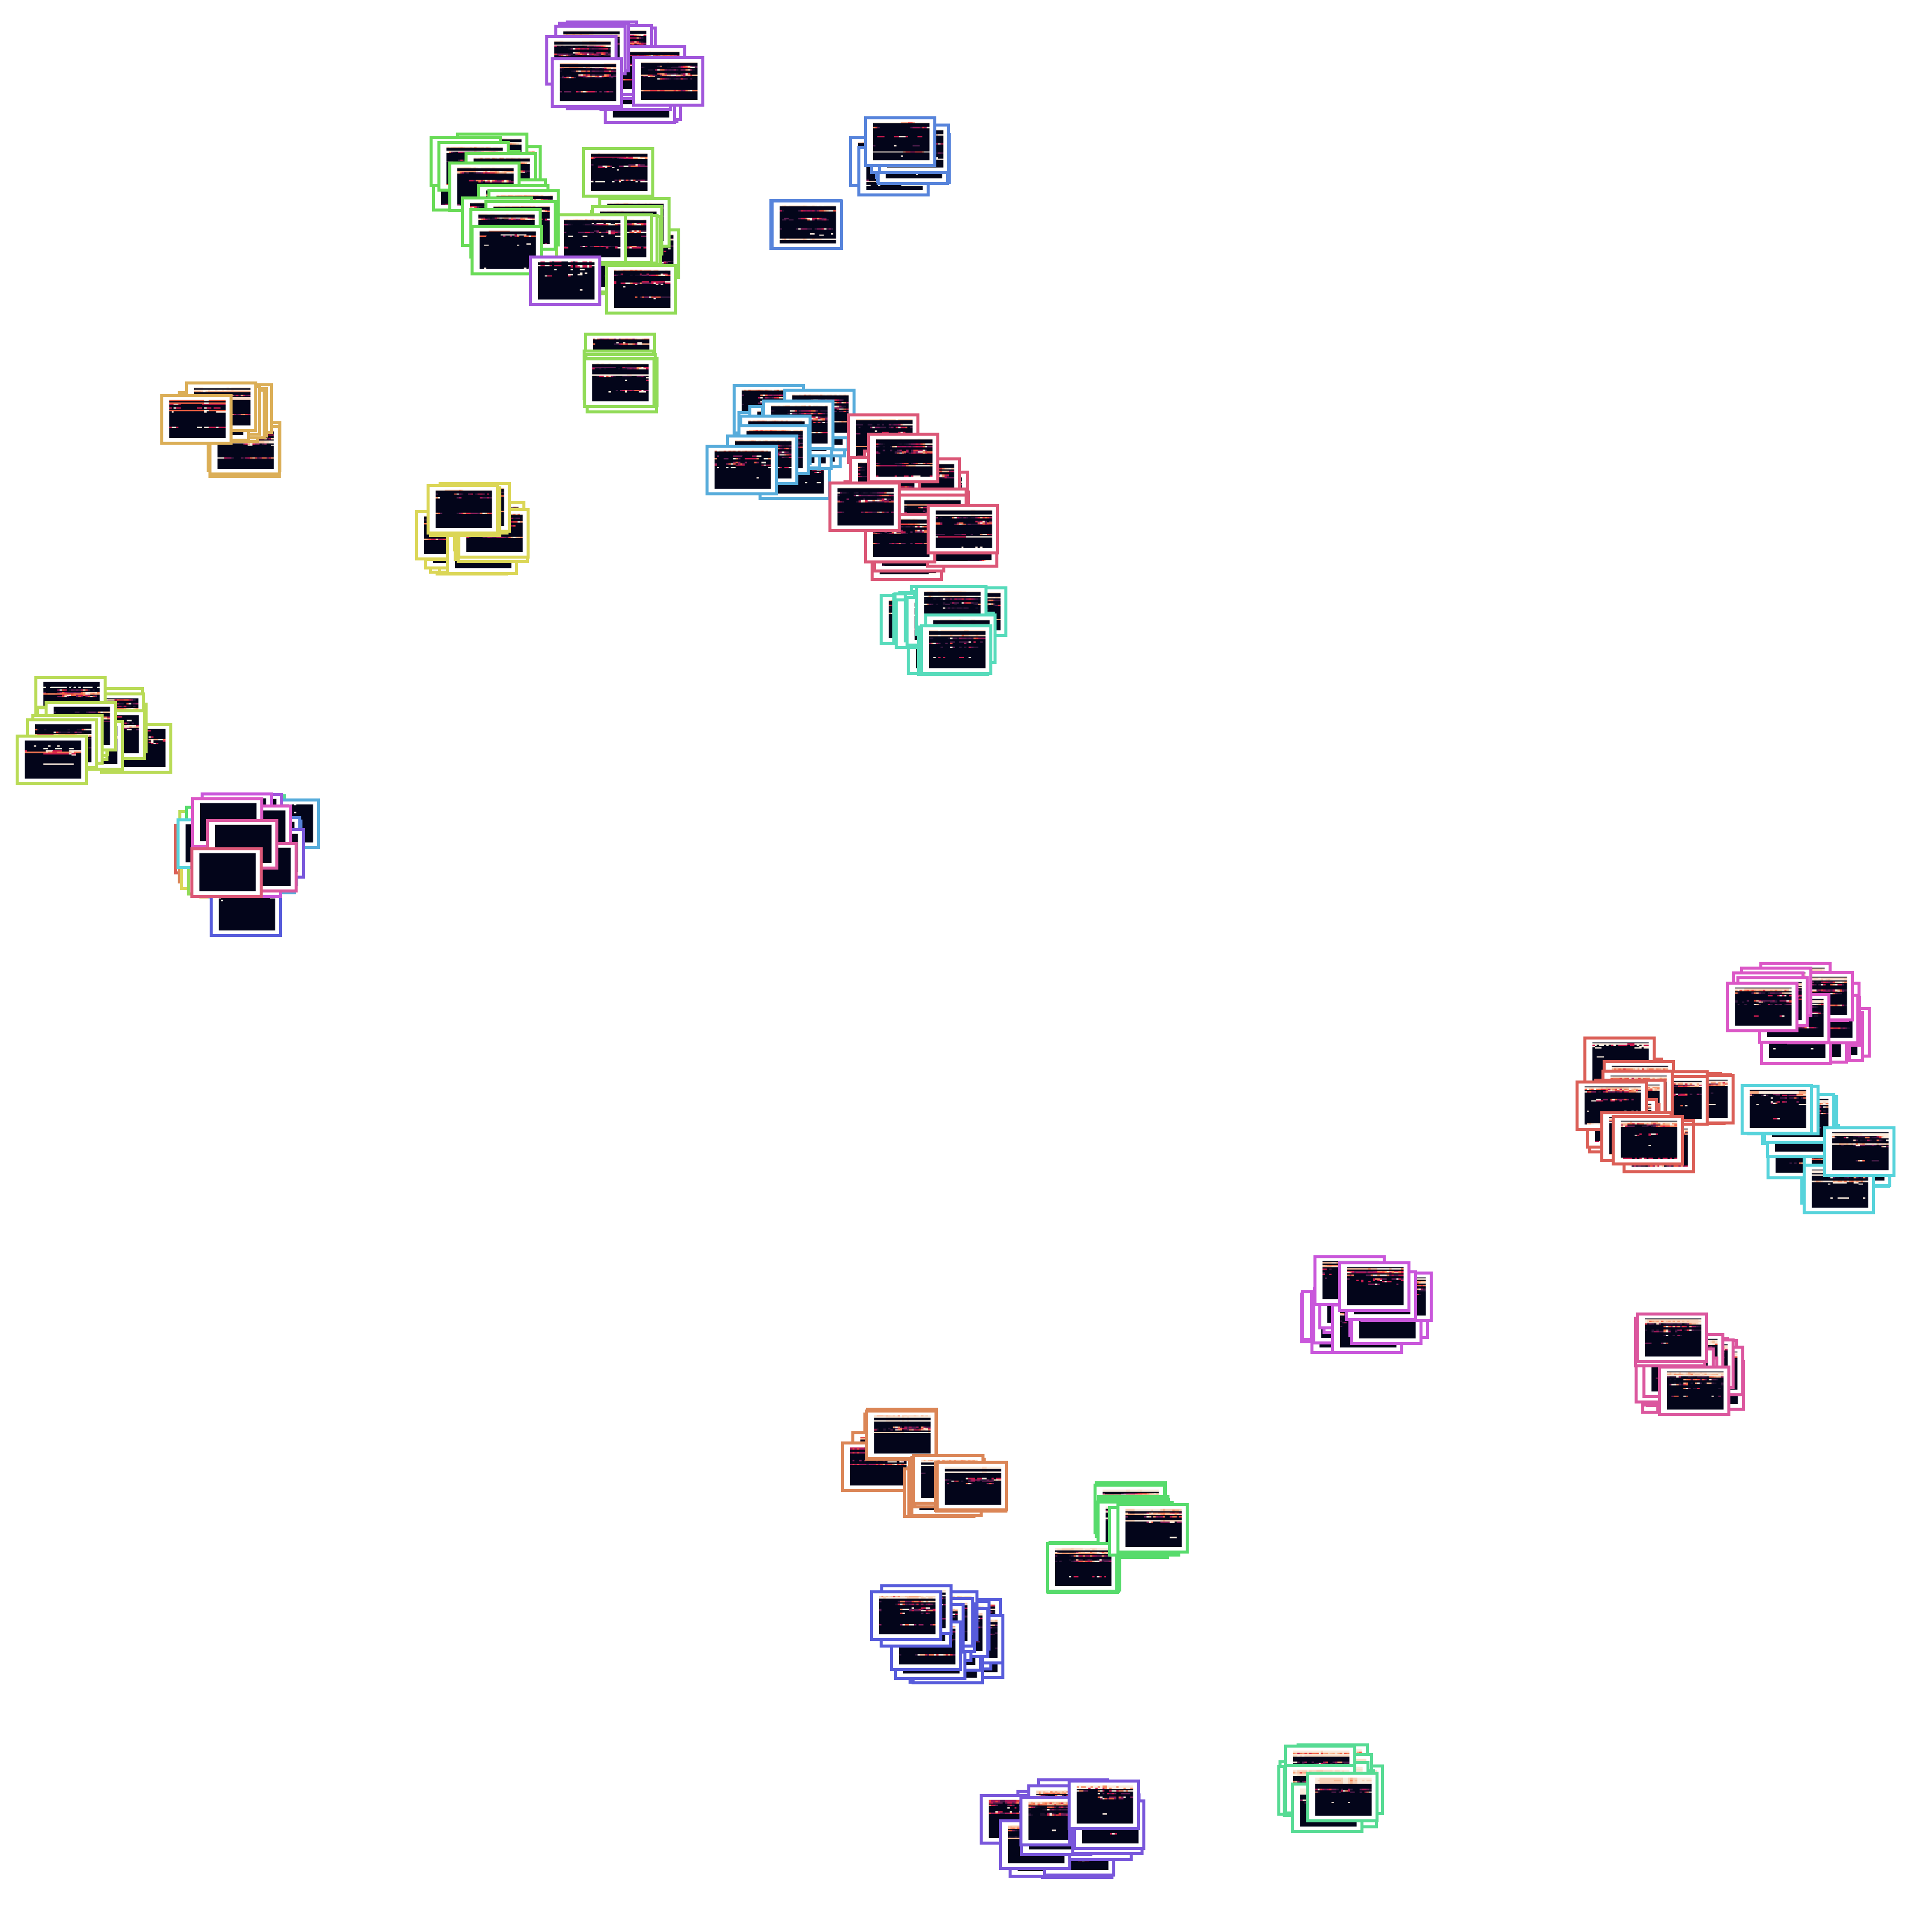
\includegraphics[width=.9\textwidth]{Figures/TSNE/TSNE_BOA/img_scatter_boa.png}
	\label{fig:tsne_boa_img_scatter_refit8}
	\par
	\par\footnotesize{Full resolution figure: \url{https://github.com/jenkoj/msc/tree/main/Figures/TSNE/TSNE_BOA/img_scatter_boa.png}}
\end{figure}

\section{Discussion}

We used t-SNE to show how LPs are related in high-dimensional space, by mapping them into two-dimensional space.
We used three different types of LPs: per-building, per-building per-appliance, a bag of appliances, and per-appliance.
Per-building load profiles offered a look into how activations patterns differ across different buildings and datasets.
Per-building per-appliance bag of appliance load profiles offered the same thing, but in greater detail.
Per-appliance load profiles were the most versatile and were utilized in the most various ways:
First, we have shown how the same type of appliance is being used across various buildings.
Next, we compared appliances with each other. 
Since the plot was hard to comprehend, we have defined appliance groups.
These new groups formed clusters, which furthermore revealed the relation between LPs. 
Finally, we compared how appliance load profiles are connected in a single building. 

One of the main findings of this chapter was the formation of appliance groups.
Such groups enable us to look into the similarity of their activation profiles and enable us to understand which groups have similar usage patterns.
Another important piece of information these groups contain is the strength of the user's routine.
The closer the samples, the more similar their activation is, which means the user has a higher routine.
Such a routine will be useful in the next chapter, where we will try to evaluate if it is strong enough to detect anomalies.

\section{Summary}

The analysis provided a look into the relationships between LPs and their consumption patterns.
We were able to group appliances into categories and found a presence of routine in the LPs
These findings will be valuable in the next chapter where we continue to explore the potential applications of LPs.


\chapter{Elderly care demo} % Main chapter title

\label{chapter6} % Change X to a consecutive number; for referencing this chapter elsewhere, use \ref{ChapterX}

%----------------------------------------------------------------------------------------
%	SECTION 1
%----------------------------------------------------------------------------------------

\section{Introduction}


Elderly care has been addressed by many EU-funded research projects since the aging population is one of the main issues the EU is facing. 
There are many solutions to this problem.
One approach is invasive such as wearables, sound sensors, IR occupancy detectors, etc. 
This approach has been addressed by thousands of publications, such as reviews \cite{elderReview1}, \cite{elderReview2} and \cite{elderReview3} show and present.

Authors \cite{elderNILM} and \cite{elderNILMDementia} tried to solve this issue using a non-invasive approach with NILM algorithms. 
In the case of a non-invasive approach, no additional meters need to be installed, since per-appliance usage can be disaggregated.
While this is practical from the "no additional equipment needed" side, it is a bit less practical from the efficiency and accuracy side, especially for larger buildings. 

There is a middle way between invasive and non-invasive approaches, such as the authors explored in \cite{elder1} and \cite{elder2}. 
It is possible to use sub-meters for each appliance and indirectly observe the usage pattern. 
The advantage of this approach is that the elder does not need to wear the device.
The disadvantage is, that new meters need to be installed for the most commonly used appliances.

Our approach will use the latter.

\section{Goal}

The chapter will focus on building an elderly care system that will use users' periodic usage patterns to detect an anomaly.
The anomaly could be anything from a fall, stroke or altered usage pattern due to dementia. 
The algorithm will be designed based on the load profile \ref{fig:PHPA}, which we discussed in chapter \ref{chapter4}.
Figure shows, that the first thing in the morning used are a kettle and toaster, and with a delay of one hour, microwave and TV. 
If none of these appliances are used within that hour, then that hour is considered anomalous.
This means that the algorithm will be able to detect the anomaly within 1 hour of the accident.

\section{Methodology}

\subsection{Defining an Anomaly}

Since the elderly care system is based on anomaly detection, we have to define it first.
In our case, the anomaly occurs when something that should operate, does not. 
Based on this definition we will develop an anomaly detection algorithm. 

\subsection{Building Anomaly Detection Algorithm}

The next section will present the steps taken while designing this algorithm.

\subsubsection{Step One}
To detect the anomalies one first needs to build a daily activation profile for each appliance, such as the one previously shown in Figure \ref{fig:PHPA}.
In this specific case, we will be using 2h buckets, yielding a total of 12 buckets. 

\subsubsection{Step Two}
The second step is to ignore appliances that are always on by calculating the standard deviation of activations for each bucket. 
The activations are normalized between 0 and 1. 
This step is important so that appliances that are always on, such as fridges or freezers get ignored. 
These appliances are detected based on the width of their activation normal distribution. 
Periodic (on an hourly basis) appliances should have narrow distributions and the more dynamic should have wider distributions.
This can be seen in examples from building 2.
\begin{figure}[H]
    \centering
    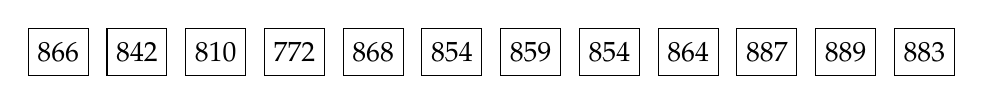
\begin{tikzpicture}
        \coordinate (s) at (0,0);
        \foreach \num in {866, 842, 810, 772, 868, 854, 859, 854, 864, 887, 889, 883}{
        \node[minimum size=6mm, draw, rectangle] at (s) {\num};
        \coordinate (s) at ($(s) + (1,0)$);
        }
    \end{tikzpicture}
    \caption{Daily activations for fridge $\sigma$ = 0.036}
    \label{arr:fridge_acts}
\end{figure}

\begin{figure}[H]
    \centering
    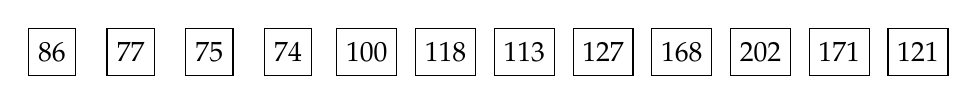
\begin{tikzpicture}
        \coordinate (s) at (0,0);
        \foreach \num in {86, 77, 75, 74, 100, 118, 113, 127, 168, 202, 171, 121}{
        \node[minimum size=6mm, draw, rectangle] at (s) {\num};
        \coordinate (s) at ($(s) + (1,0)$);
        }
    \end{tikzpicture}
    \caption{Daily activations for audio system $\sigma$ = 0.2}
    \label{arr:as_acts}
\end{figure}

\begin{figure}[H]
    \centering
    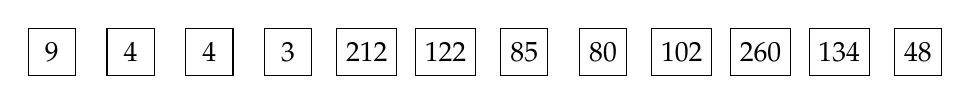
\begin{tikzpicture}
        \coordinate (s) at (0,0);
        \foreach \num in {9, 4, 4, 3, 212, 122, 85, 80, 102, 260, 134, 48}{
        \node[minimum size=6mm, draw, rectangle] at (s) {\num};
        \coordinate (s) at ($(s) + (1,0)$);
        }
    \end{tikzpicture}
    \caption{Daily activations for microwave $\sigma$ = 0.3}
    \label{arr:microwave_acts}
\end{figure}

Based on results from all appliances a threshold of $\sigma$ = 0.1 was set.
This method will also get rid of appliances that are always on due to their specific nature such as server computers 
or fridges. 

\subsubsection{Step Three}

Next, appliances that trigger together must be grouped. 
This means we must find part of the day that they are operating together.
Due to the filter in the previous step, we are left with appliances whose usage variate throughout the day. 
Some appliances are on even when the user is not necessarily using them, this can be seen in figure \ref{arr:as_acts}.
One of many ways to do this is to normalize the activations, this yields a metric that tells us the probability of that appliance being turned on compared to the rest of the day. 
If we do this for the same appliances as above the result is the following: 

\begin{figure}[H]
    \centering
    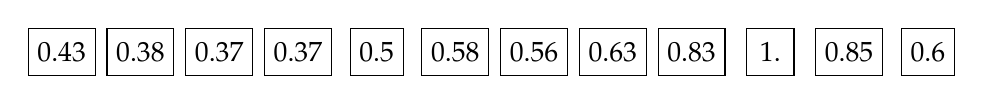
\begin{tikzpicture}
        \coordinate (s) at (0,0);
        \foreach \num in {0.43, 0.38, 0.37, 0.37, 0.5 , 0.58, 0.56, 0.63, 0.83, 1. , 0.85,
        0.6}{
        \node[minimum size=6mm, draw, rectangle] at (s) {\num};
        \coordinate (s) at ($(s) + (1,0)$);
        }
    \end{tikzpicture}
    \caption{Daily activations for audio system $\sigma$ = 0.2}
    \label{arr:as_acts_norm}
\end{figure}

\begin{figure}[H]
    \centering
    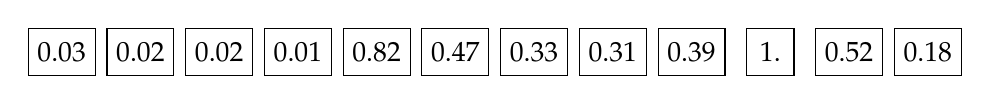
\begin{tikzpicture}
        \coordinate (s) at (0,0);
        \foreach \num in {0.03, 0.02, 0.02, 0.01, 0.82, 0.47, 0.33, 0.31, 0.39, 1.  , 0.52,
        0.18}{
        \node[minimum size=6mm, draw, rectangle] at (s) {\num};
        \coordinate (s) at ($(s) + (1,0)$);
        }
    \end{tikzpicture}
    \caption{Daily activations for microwave $\sigma$ = 0.3}
    \label{arr:microwave_acts_norm}
\end{figure}

Finally, a suitable threshold must be selected.
The threshold of 0.5 was selected, which yields the following vectors:

\begin{figure}[H]
    \centering
    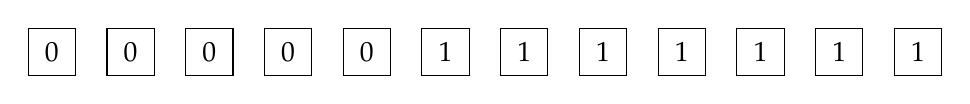
\begin{tikzpicture}
        \coordinate (s) at (0,0);
        \foreach \num in {0, 0, 0, 0, 0 , 1, 1, 1, 1, 1 , 1, 1}{
        \node[minimum size=6mm, draw, rectangle] at (s) {\num};
        \coordinate (s) at ($(s) + (1,0)$);
        }
    \end{tikzpicture}
    \caption{Daily activations for audio system}
    \label{arr:as_acts_vec}
\end{figure}

\begin{figure}[H]
    \centering
    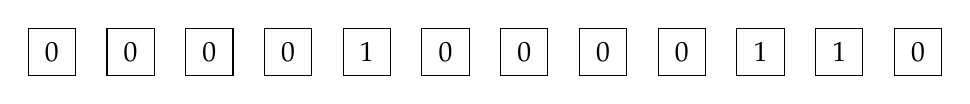
\begin{tikzpicture}
        \coordinate (s) at (0,0);
        \foreach \num in {0, 0, 0, 0, 1, 0, 0, 0, 0, 1, 1, 0}{
        \node[minimum size=6mm, draw, rectangle] at (s) {\num};
        \coordinate (s) at ($(s) + (1,0)$);
        }
    \end{tikzpicture}
    \caption{Daily activations for microwave with one usage peak in the morning and the other in the evening}
    \label{arr:microwave_acts_vec}
\end{figure}

The vectors show us that the microwave has two usage peaks, where the audio system can be used anytime throughout the day.
It is possible to do this for all appliances, which results in a 2D matrix. 
Using this matrix we can build rules for which appliances are being used together.
Figure \ref{arr:act_mat} uses rows for appliances and columns for buckets.  
If we use terminology from image processing the matrix \ref{arr:act_mat} is essentially a highly saturated load profile \ref{fig:PHPA},
which can be easily processed by computer algorithms due to binary encoding. 

\begin{figure}[H]
    \centering
    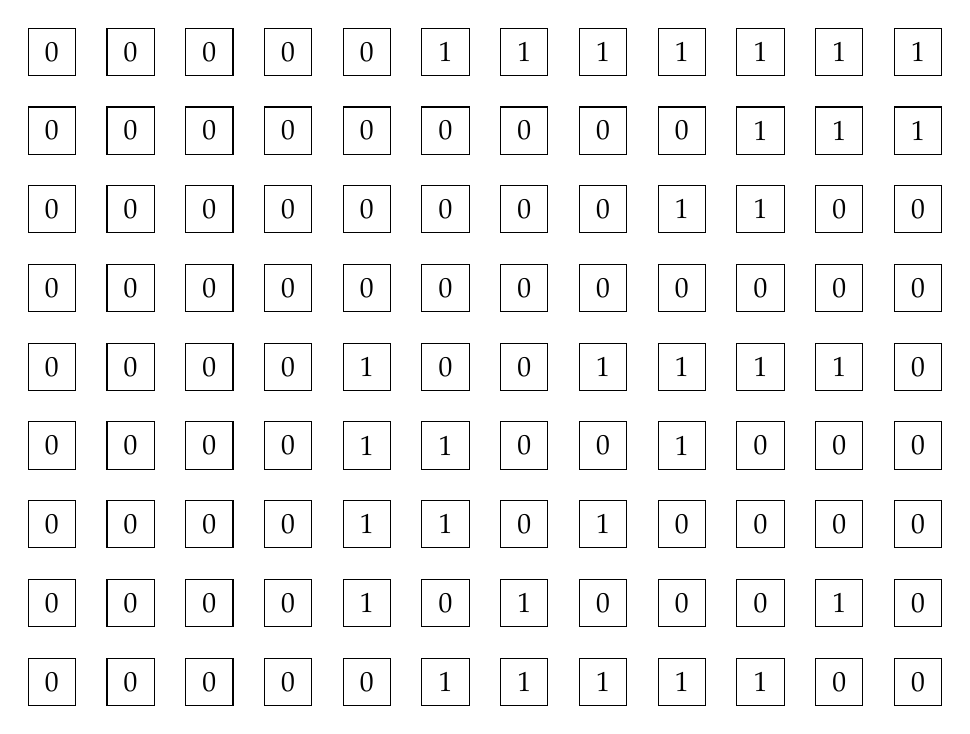
\begin{tikzpicture}
        \coordinate (s) at (0,8);
        \foreach \num in {0, 0, 0, 0, 0, 1, 1, 1, 1, 1, 1, 1}{
        \node[minimum size=6mm, draw, rectangle] at (s) {\num};
        \coordinate (s) at ($(s) + (1,0)$);
        }
        \coordinate (s) at (0,7);
        \foreach \num in {0, 0, 0, 0, 0, 0, 0, 0, 0, 1, 1, 1}{
        \node[minimum size=6mm, draw, rectangle] at (s) {\num};
        \coordinate (s) at ($(s) + (1,0)$);
        }
        \coordinate (s) at (0,6);
        \foreach \num in {0, 0, 0, 0, 0, 0, 0, 0, 1, 1, 0, 0}{
        \node[minimum size=6mm, draw, rectangle] at (s) {\num};
        \coordinate (s) at ($(s) + (1,0)$);
        }
        \coordinate (s) at (0,5);
        \foreach \num in {0, 0, 0, 0, 0, 0, 0, 0, 0, 0, 0, 0}{
        \node[minimum size=6mm, draw, rectangle] at (s) {\num};
        \coordinate (s) at ($(s) + (1,0)$);
        }
        \coordinate (s) at (0,4);
        \foreach \num in {0, 0, 0, 0, 1, 0, 0, 1, 1, 1, 1, 0}{
        \node[minimum size=6mm, draw, rectangle] at (s) {\num};
        \coordinate (s) at ($(s) + (1,0)$);
        }
        \coordinate (s) at (0,3);
        \foreach \num in {0, 0, 0, 0, 1, 1, 0, 0, 1, 0, 0, 0}{
        \node[minimum size=6mm, draw, rectangle] at (s) {\num};
        \coordinate (s) at ($(s) + (1,0)$);
        }
        \coordinate (s) at (0,2);
        \foreach \num in {0, 0, 0, 0, 1, 1, 0, 1, 0, 0, 0, 0}{
        \node[minimum size=6mm, draw, rectangle] at (s) {\num};
        \coordinate (s) at ($(s) + (1,0)$);
        }
        \coordinate (s) at (0,1);
        \foreach \num in {0, 0, 0, 0, 1, 0, 1, 0, 0, 0, 1, 0}{
        \node[minimum size=6mm, draw, rectangle] at (s) {\num};
        \coordinate (s) at ($(s) + (1,0)$);
        }
        \coordinate (s) at (0,0);
        \foreach \num in {0, 0, 0, 0, 0, 1, 1, 1, 1, 1, 0, 0}{
        \node[minimum size=6mm, draw, rectangle] at (s) {\num};
        \coordinate (s) at ($(s) + (1,0)$);
        }
    \end{tikzpicture}
    \caption{Activation matrix}
    \label{arr:act_mat}
\end{figure}

It is possible to display the matrix \ref{arr:act_mat} as an image.
The Figure below shows how the load profile is transformed.

\begin{figure}[H]
	\begin{subfigure}{.5\textwidth}
		% \centering
		\caption{Input data}
		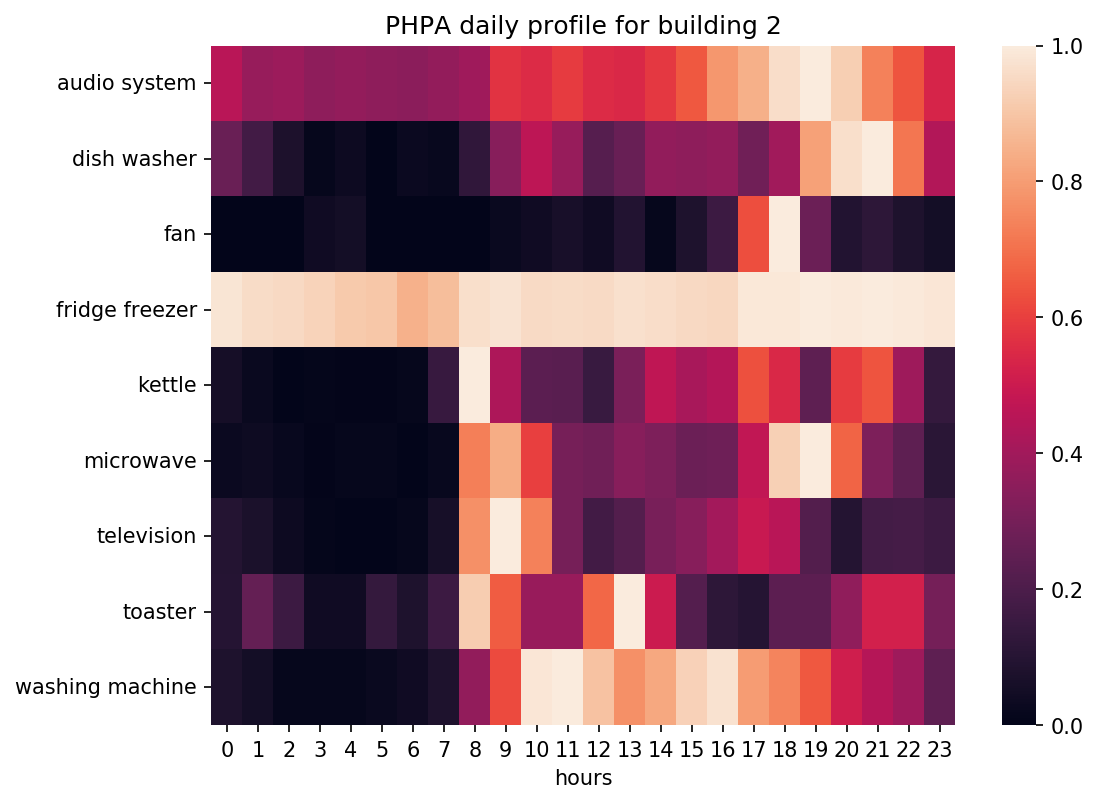
\includegraphics[width=1\linewidth]{../Figures/LPS/PHPA.png}
		\label{fig:ec_PHPA}
	\end{subfigure}%
	~ 
	\begin{subfigure}{.5\textwidth}
		% \centering
		\caption{Figure \protect\ref{arr:act_mat} as an image}
		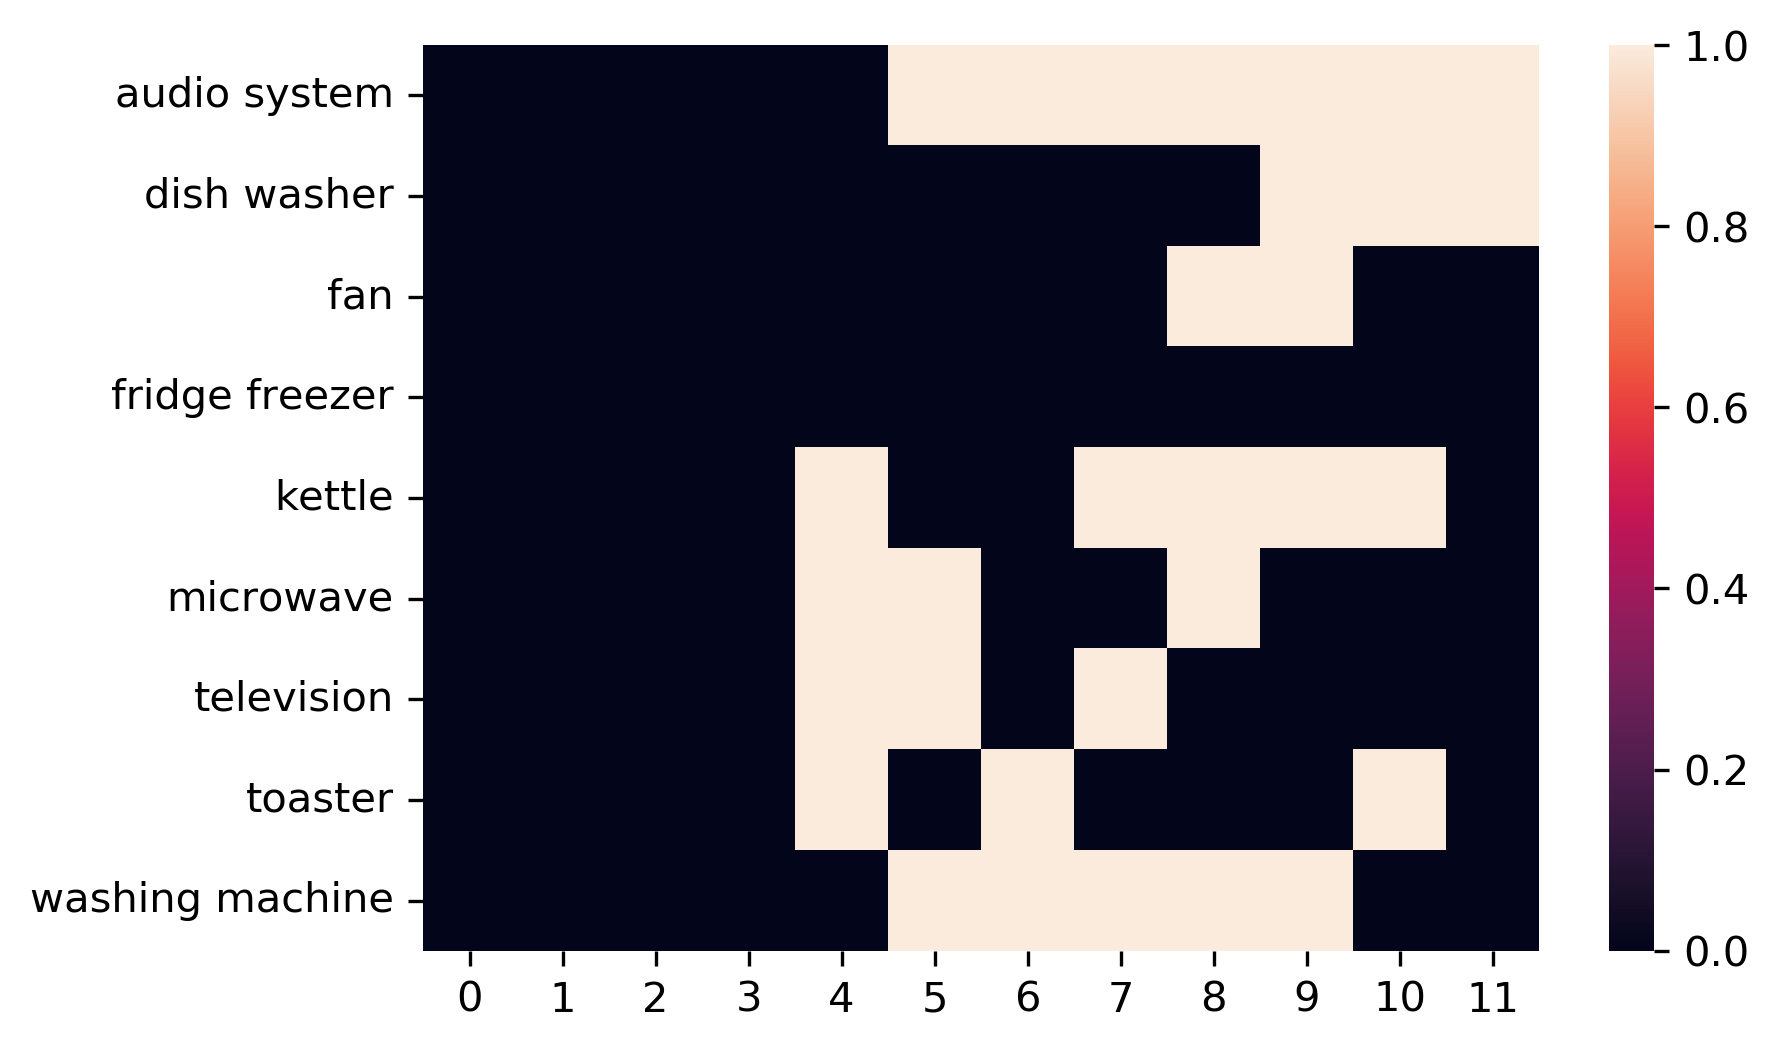
\includegraphics[width=1\linewidth]{../Figures/LPS/PHPA_EC.png}
		\label{fig:ec_PHPA_bw}
	\end{subfigure}%

	\caption{Transformation of source load profile to black and white}
\end{figure}

\subsubsection{Step Four}

Previously, we have defined that an anomaly occurs when something that should activate does not.
Using the matrix \ref{arr:act_mat} we can compile an algorithm that will detect the anomaly using current activations being tested 
and comparing it to the adjacent column in matrix \ref{arr:act_mat}.
Let us use the fifth bucket as an example. That is data from 8 to 10 o'clock.

The tested sample is considered normal if at least two appliances that are normally being used are activated.
Otherwise, the tested sample is considered anomalous.
Our implementation multiplies the adjacent matrix column to the tested sample.
We sum the elements of the resulting array and check if it is larger or equal to 2.
If cases where this rule is false, samples are considered anomalous.

\begin{figure}[H]
    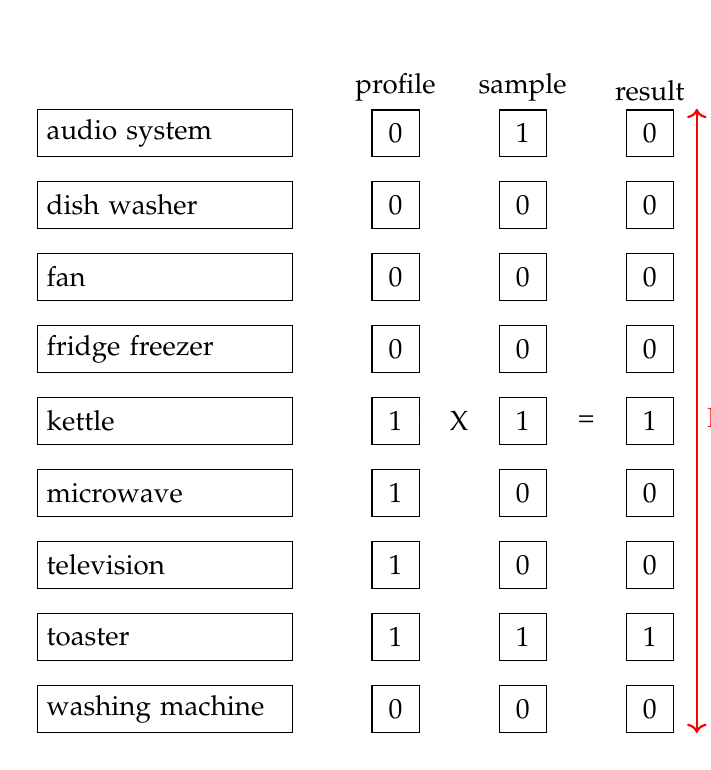
\begin{tikzpicture}
      \matrix [row sep=3mm, column sep=1cm,nodes={minimum size=6mm, draw, rectangle}]
      {
      \node[text width=3cm,white] {margin};\\ 
      \node[text width=3cm] {audio system}; &  \node (t1){0}; & \node  (t2){1}; & \node (s1){0};\\
      \node[text width=3cm] {dish washer}; &   \node     {0}; & \node     {0}; & \node     {0};\\
      \node[text width=3cm] {fan}; &           \node     {0}; & \node     {0}; & \node     {0};\\
      \node[text width=3cm] {fridge freezer}; &\node     {0}; & \node     {0}; & \node     {0};\\
      \node[text width=3cm] {kettle}; &        \node (a) {1}; & \node (b) {1}; & \node (c) {1};\\
      \node[text width=3cm] {microwave}; &     \node     {1}; & \node     {0}; & \node     {0};\\
      \node[text width=3cm] {television}; &    \node     {1}; & \node     {0}; & \node     {0};\\
      \node[text width=3cm] {toaster}; &       \node     {1}; & \node     {1}; & \node     {1};\\
      \node[text width=3cm] {washing machine}; &\node    {0}; & \node     {0}; & \node (s2){0};\\
      };
      \draw [<->,white] (a.east) -- (b.west) node[black] [midway] {X};
      \draw [<->,white] (b.east) -- (c.west) node[black] [midway] {=};
    
      \begin{scope}[transform canvas={yshift=0.8em}]
      \draw [-] (t1.west) -- (t1.east)node[black] [above,midway] {profile};
      \end{scope}
    
      \begin{scope}[transform canvas={yshift=0.8em}]
      \draw [-] (t2.west) -- (t2.east)node[black] [above,midway] {sample};
      \end{scope}
    
      \begin{scope}[transform canvas={yshift=0.8em}]
      \draw [-] (s1.west) -- (s1.east)node[black] [above,midway] {result};
      \end{scope}
    
      \begin{scope}[transform canvas={xshift=1.7em}]
       \draw [<->,red,thick] (s1.north) -- (s2.south) node [right,midway] {IF SUM >= 2 not an anomaly};
      \end{scope}
    \end{tikzpicture}
    \caption{The evaluation of the test sample compared to the adjacent column from the matrix. An example is for a fifth bucket or fifth row from the matrix.}
    
\end{figure}

% \begin{figure}[H]
%     \centering
%     \caption{Process of evaluating an anomaly}
%     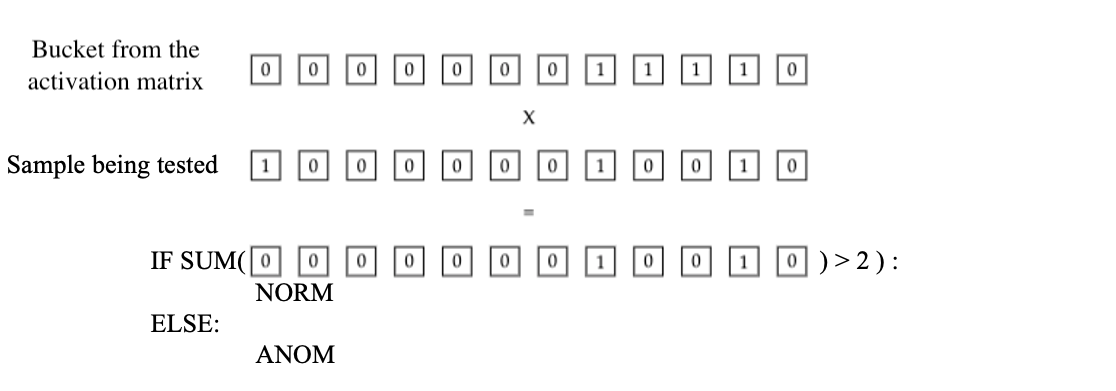
\includegraphics[width=1\linewidth]{../Figures/EC/EC_anom_dect.png}
%     \label{fig:anom_detct}
%     \caption{The evaluation of new bucket compared to matrix. An example is for a fifth bucket or fifth row from the matrix.}
    
% \end{figure}

This process is done for all samples, where we count normal and anomalous samples for each bucket
The important thing to note here is that we are evaluating the samples from train data, from which the profile was built.

\begin{figure}[H]
    \centering
    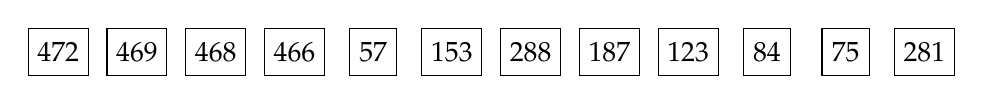
\begin{tikzpicture}
        \coordinate (s) at (0,0);
        \foreach \num in {472, 469, 468, 466, 57, 153, 288, 187, 123, 84, 75, 281}{
        \node[minimum size=6mm, draw, rectangle] at (s) {\num};
        \coordinate (s) at ($(s) + (1,0)$);
        }
    \end{tikzpicture}
    \caption{Aggregated anomalies for each bucket}
    \label{arr:agg_anom}
\end{figure}

\begin{figure}[H]
    \centering
    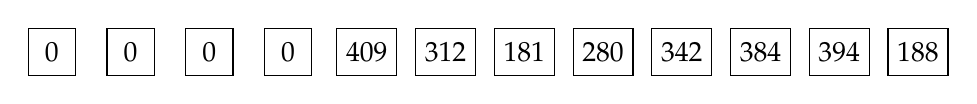
\begin{tikzpicture}
        \coordinate (s) at (0,0);
        \foreach \num in {0, 0, 0, 0, 409, 312, 181, 280, 342, 384, 394, 188}{
        \node[minimum size=6mm, draw, rectangle] at (s) {\num};
        \coordinate (s) at ($(s) + (1,0)$);
        }
    \end{tikzpicture}
    \caption{Aggregated normal samples for each bucket}
    \label{arr:agg_norm}
\end{figure}

\subsubsection{Step Five}

The next step is to combine these two arrays so that we calculate the percentage of anomalous samples 
for each bucket with an equation. 

\begin{equation}
    \frac{N_{anom}}{N_{anom}+N_{norm}}
    \label{eq:ratio}
\end{equation}

Where $N_{anom}$ is a number of anomalous samples and $N_{norm}$ is a number of normal samples.


We can alter the equation \ref{eq:ratio} so that it will measure
a number of normal samples out of all. 
The result is the equation \ref{eq:routine}
In other words, we are measuring the strength of a routine that 
user has in each bucket.

\begin{equation}
    R_{outine}= \frac{N_{norm}}{N_{anom}+N_{norm}}
    \label{eq:routine}
\end{equation}

Using the equation \ref{eq:routine} we can populate the array \ref{arr:anom_ratio}.

\begin{figure}[H]
    \centering
    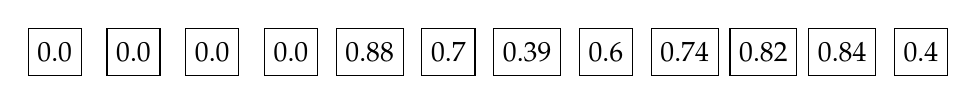
\begin{tikzpicture}
        \coordinate (s) at (0,0);
        \foreach \num in {0.0, 0.0, 0.0, 0.0, 0.88, 0.7, 0.39, 0.6, 0.74, 0.82, 0.84, 0.4}{
        \node[minimum size=6mm, draw, rectangle] at (s) {\num};
        \coordinate (s) at ($(s) + (1,0)$);
        }
    \end{tikzpicture}
    \caption{Aggregated anomalies for each bucket}
    \label{arr:anom_ratio}
\end{figure}

In other words, the array \ref{arr:anom_ratio} tells us how persistent is the user's routine in each bucket or part of the day. 
The higher the metric the higher the routine. 
Since routine is detected based on the usage of appliances it cannot be picked up during the night.

It is possible to see that the routine is quite high during the morning and evening hours.
The anomaly detection algorithm will work best when the metric above is high.
A good trait of the elderly is that their routine is quite high even during the day.

One more thing to do is to ignore the parts of the day when the user has no routine.
This is done by using the array \ref{arr:anom_ratio} and setting a threshold of 0.7. 

A threshold of 0.5 would mean that we could detect false positive anomalies every other day.
Setting the rate to 0.7 reduces this to every third day.
Here, compromises must be made, the lower the threshold the more accurate the algorithm will be. 
This also means that it will be less sensitive. 
In our case, there is not much harm in false positive detections, since the caregiver can call the elder to check if it is okay.  

\begin{figure}[H]
    \centering
    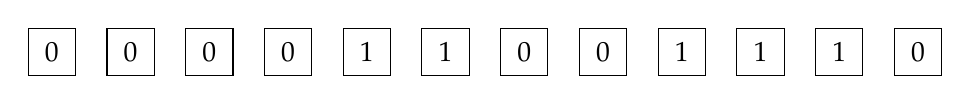
\begin{tikzpicture}
        \coordinate (s) at (0,0);
        \foreach \num in {0, 0, 0, 0, 1, 1, 0, 0, 1, 1, 1, 0}{
        %\foreach \num in {1.0, 1.0, 1.0, 1.0, 0.12, 0.3, 0.61, 0.4, 0.26, 0.18, 0.16, 0.6}{
        \node[minimum size=6mm, draw, rectangle] at (s) {\num};
        \coordinate (s) at ($(s) + (1,0)$);
        }
    \end{tikzpicture}
    \caption{Using the above-mentioned threshold a new mask is made, to check only buckets with high routine.}
    \label{arr:anom_ratio_mask}
\end{figure}

\subsubsection{Step Six}

The last step is to repeat steps 4 and 5 with test data.
When using test data, we skip the buckets with low routine rates by using the mask on Figure \ref{arr:anom_ratio_mask}.
Since the profile has never seen the data being used, this should give us a good presentation of actual performance in a real-world scenario.
\subsection{Datasets and evaluation} \label{ssec:ds_eval}

The data was split into train and test sets, where 80 \% of the data was used for training and 20 \% percent of the data for testing.
The data was split based on the number of samples, so in some cases where there is a lot of missing data, the time window of test data might be longer, although it contains only 20 \% of the samples.

\subsubsection{REFIT}
The REFIT \cite{REFIT} dataset included data for more than 15 buildings, as can be seen in the Figure below.
The dataset in general is of the highest quality since it is the longest with the least missing data.
This means this dataset should give the most relevant results.
\begin{figure}[H]
	\centering
	\caption{Timeline for REFIT}
	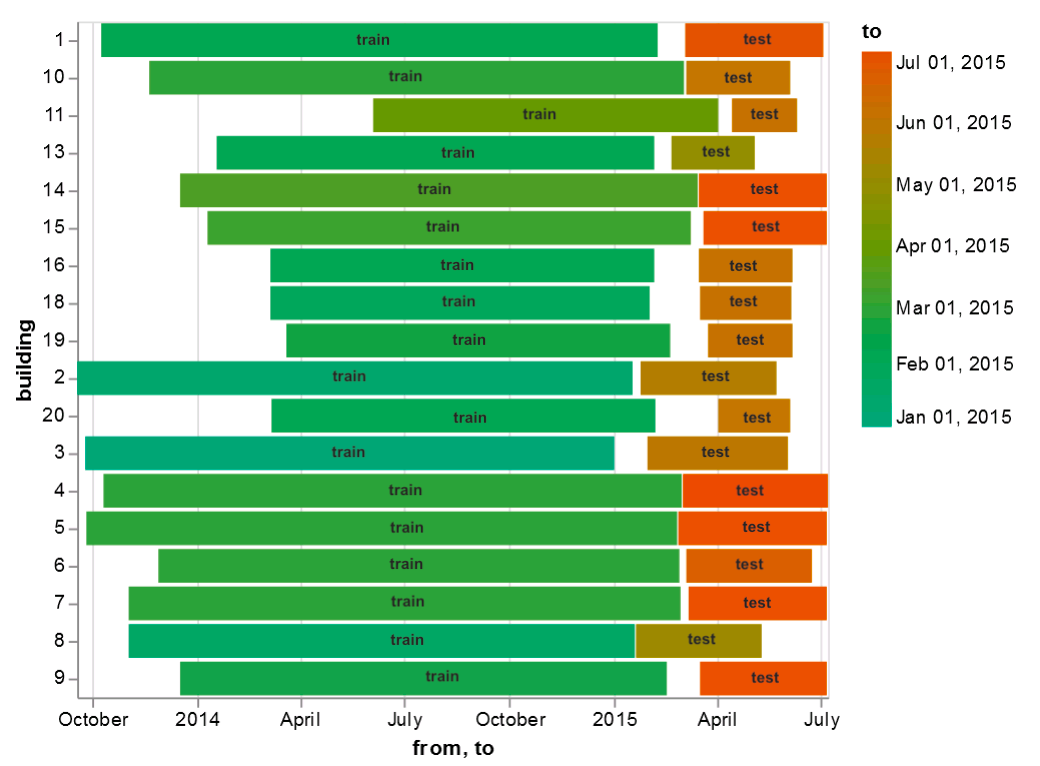
\includegraphics[width=1\textwidth]{Figures/EC/refit_timeline.png}
	\label{fig:refit_timeline}
\end{figure}

\subsubsection{UK-DALE} 

Through the UK-DALE \cite{UKDALE} dataset is of similar size, most of the data is from building 1.
In general, it includes 5 years of data, but only for some appliances, where many appliances are rarely used.
When taking all of this into account, there were too many issues with building 1, and it was simply ignored.
Another issue that can be seen in Figure \ref{fig:ukdale_timeline} is that there is not enough data for 
building 3. The test includes only a week of data, which is not enough for representative results, therefore it was ignored.
The rest of the buildings seem healthy.

\begin{figure}[H]
	\centering
	\caption{Timeline for UK-DALE}
	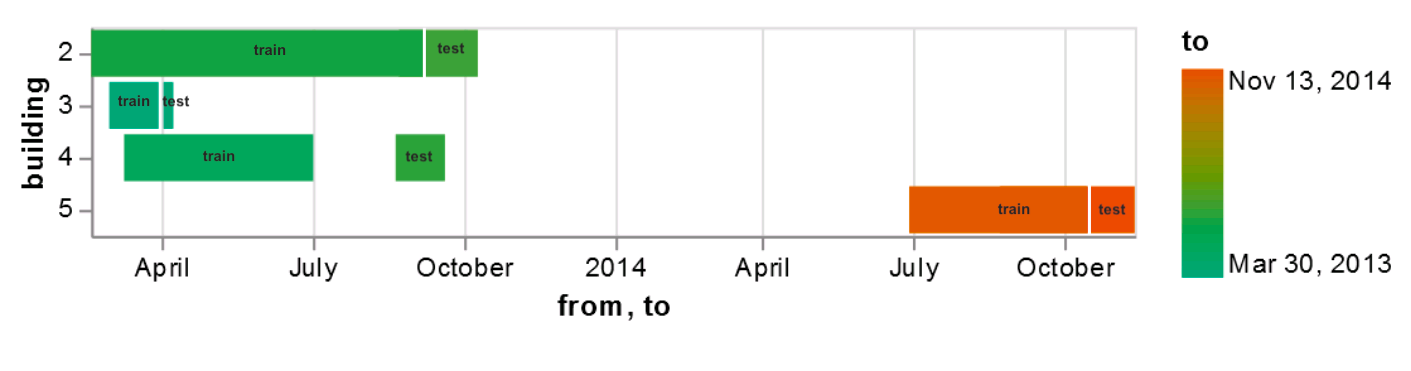
\includegraphics[width=1\textwidth]{Figures/EC/ukdale_timeline.png}
	\label{fig:ukdale_timeline}
\end{figure}

\subsubsection{ECO}
ECO \cite{ECO} dataset has a length of data similar to UK-DALE. 
The only issue is building 1, where there is a lot of missing data.
This is a good example of how data is split, it is split based on several samples,
meaning that there is 80 \% in the train bar, due to missing data the second bar is longer. 

\begin{figure}[H]
	\centering
	\caption{Timeline for ECO}
	\includegraphics[width=1\textwidth]{Figures/EC/eco_timeline.png}
	\label{fig:eco_timeline}
\end{figure}


\subsection{The metric - routine rate}

Due to the lack of ground truth data of actual accidents, it is hard to determine the 
exact accuracy of this algorithm. Every anomaly detected is not necessarily an 
actual accident, it could be that the user decided to lie in bed a bit longer, or decided to go to bed early in the evening.
One metric that we can use to determine how well the algorithm functions is the routine rate metric \ref{arr:anom_ratio}.
The reason behind that is, that if the routine rate is high it means that it will be easier to detect the actual anomaly.

\begin{itemize}
	\item Routine rate of 0 would mean that for that bucket household has no routine at all.
    \item Routine rate of 0.5 would mean that the routine is broken every second day.
    \item Routine rate of 0.8 would mean that routine is broken on average every fifth day.
    \item Routine rate of 1 would mean that this household has a routine that is never broken. 
\end{itemize}

An example of when a user routine rate is close to 1. When a true anomaly occurs such as a fall, the dweller, though he had the same strong routine for the past year, would not be able to practice it, and the algorithm will be quite sure that this is an actual anomaly.
Therefore, the lower the routine rate the less sure we are that an actual anomaly such as a fall occurred.
This is a good alternative measurement, that tells us how well this algorithm will perform. 
Since sometimes it is easier to read when results are presented with percentages, we will sometimes use this way of presenting it.
 
\section{Results} 

Results were obtained for 3 datasets. 
REDD and iAWE datasets were not used, since they were too small. 
They contained less than a month of data. 

\subsection{The Routine Rate Over a Period of Time}

In the following sections, we will present how the metric changes over given periods of time.
This will enable us to see that there are patterns that this metric helps reveal. 
Since we have more than a year of training data, this will enable us to see how the metric changes over years.
This enables us to see how routine changes over the year. 
We cannot use testing data in this case, since there is not enough of it.

\subsubsection{The Routine Rate Through the Week} \label{sssec:ratio_week}

As the behavior of the dweller changes, so does the accuracy of the algorithm. 
One observation that was made, was that the routine was higher during the week than during the weekends,
as can be seen in the Figure \ref{fig:ec_week} below. 
The only exception is Figure \ref{fig:ec_b5week}, which shows that the observation does not hold for all houses. 

\begin{figure}[H]
	\begin{subfigure}{.5\textwidth}
		% \centering
		\caption{Building 2}
		\includegraphics[width=1\linewidth]{../Figures/EC/b2week.png}
		\label{fig:ec_b2week}
	\end{subfigure}%
	~ 
	\begin{subfigure}{.5\textwidth}
		% \centering
		\caption{Building 19}
		\includegraphics[width=1\linewidth]{../Figures/EC/b19week.png}
		\label{fig:ec_b19week}
	\end{subfigure}%
    \bigskip

    \begin{subfigure}{.5\textwidth}
		% \centering
		\caption{Building 18}
		\includegraphics[width=1\linewidth]{../Figures/EC/b18week.png}
		\label{fig:ec_b18week}
	\end{subfigure}%
    ~ 
    \begin{subfigure}{.5\textwidth}
		% \centering
		\caption{Building 5}
		\includegraphics[width=1\linewidth]{../Figures/EC/b5weekd.png}
		\label{fig:ec_b5week}
	\end{subfigure}%
	\caption{Routine rate through the week (train data)}
    \label{fig:ec_week}
\end{figure}


Since we are dealing with the elderly, they have a higher routine, and it does not change that much during the weekends. 
Usually, assisted living systems are put in place since elders are alone in the dwelling.
Taking all of this into account, we could assume that the routine of the elderly is the same trough the week and simply ignore the weekends. 
This should yield more relevant results. 

\subsubsection{Routine Rate Through a Year}

The rate at which the routine is being practiced also changes over a year. 
While on average the routine rate is higher during the winter, spring and fall, it is lower during the summer, due to vacation. 
This can be seen in Figure \ref{fig:ec_year} below. 
It is possible to observe dips in routine. 
In some cases, these dips occur in summer and others in springtime. 
Without metadata, we cannot know for sure, what was the event behind these dips. 
There is a high chance most of them are vacations or other events where one or more dwellers are away from home for extended periods of time. 

\begin{figure}[H]
	\begin{subfigure}{.5\textwidth}
		% \centering
		\caption{Building 2}
		\includegraphics[width=1\linewidth]{../Figures/EC/b2year.png}
		\label{fig:ec_b2year}
	\end{subfigure}%
	~ 
	\begin{subfigure}{.5\textwidth}
		% \centering
		\caption{Building 19}
		\includegraphics[width=1\linewidth]{../Figures/EC/b19year.png}
		\label{fig:ec_b19year}
	\end{subfigure}%
    \bigskip

    \begin{subfigure}{.5\textwidth}
		% \centering
		\caption{Building 18}
		\includegraphics[width=1\linewidth]{../Figures/EC/b18year.png}
		\label{fig:ec_b18year}
	\end{subfigure}%
    ~ 
    \begin{subfigure}{.5\textwidth}
		% \centering
		\caption{Building 5}
		\includegraphics[width=1\linewidth]{../Figures/EC/b5year.png}
		\label{fig:ec_b5year}
	\end{subfigure}%
	
	\caption{Routine through the year (train data)}
    \label{fig:ec_year}
\end{figure}

\subsubsection{Effectiveness of Anomaly Detection Through the Day}

The following subsection will show how the effectiveness of anomaly detection changes throughout the day.

One thing to keep in mind is that this algorithm can detect anomalies only when
the routine is high, and when more than two appliances are used in given buckets.

Figure \ref{fig:ignored_buckets_22} shows which buckets are most commonly used for the detection of an anomaly.
The graph includes averaged values from all buildings and datasets. 
In other words, the graph presents how strong is average routine throughout the day.

This means that the higher the routine, the higher the chance that this bucket will be used for anomaly detection.
During the night, it is possible to see that the average routine rate is quite high.
This can be seen in Figure \ref{fig:ignored_buckets_22}
this is because most users are routinely sleeping during that period.
As we can see in Figure \ref{fig:ignored_buckets_22},
the high routine rate does not necessarily mean the buckets are useful.

\begin{figure}[H]
	\centering
	\caption{Effectivity of anomaly detection through the day}
	\includegraphics[width=.8\textwidth]{Figures/EC/ignored_buckets_dist.png}
	\label{fig:ignored_buckets_22}
\end{figure}

To find the usable buckets, an additional filter must be applied.
The rule is that at least two appliances must be commonly used in that bucket. 
After applying this rule the following Figure emerges \ref{fig:ignored_buckets_act}

\begin{figure}[H]
	\centering
	\caption{Actual effectiveness of anomaly detection through the day}
	\includegraphics[width=.8\textwidth]{Figures/EC/all_ignored_buckets_dist_incl_act.png}
	\label{fig:ignored_buckets_act}
\end{figure}

Figure \ref{fig:ignored_buckets_act} shows that there are two peaks.
One in the morning and the other, a wider one, in the evening.

This means that on an average home the algorithm would perform best in the morning and evening because the average person is at school or work during noon. 
The elderly, are usually at home at noon, which could extend the effective detection window.


\subsubsection{The Anomaly Detection During the Night}

We have seen that anomalies can be detected throughout the day,
but are hard to detect through the night, since appliances are off.

This is because, in our current state, an anomaly occurs when something that should operate, does not.
When the user is sleeping, an anomaly occurs when something that shouldn't operate, does. 
To implement this additional rule, we would have to build two models.
One would be online during the day, and the other when the user is sleeping.

To obtain information about the user's sleep schedule, we could either have a schedule obtained from the user or we could extract it based on the usage pattern of appliances.
It is possible to detect when most of the appliances are inactive and build a sleep profile based on this information.

Using the sleep schedule, it is possible to switch between the two operating modes. 
This new implementation would further extend the time windows within which we can detect the anomalies and thus further improve users' safety.

The main issue is not the detection itself but efficiently detecting
when the user is sleeping. 

The examples above were a demonstration and a look into data and metrics. 
The examples shown were trained and evaluated on the same data. 
To show true performance, we will use test data to determine the actual performance. 


\subsection{Per-Building Results}
\subsubsection{REFIT}

Results show, that the method is on average 76.4 \% efficient for REFIT.  
In Figure \ref{fig:refit_res} it is possible to see that building 8 yields much better results than the rest.
Results show that the building reached a routine rate of almost 100 \%, which is highly unlikely in the real world. 
On the contrary, buildings 11 and 13 performed much worse than the others with routine rates of around 40 \%.
It is hard to know the exact reasons why the buildings performed in such a way.
This could be due to various dataset errors that occurred during sampling.

\begin{figure}[H]
	\centering
	\caption{Results for REFIT}
	\includegraphics[width=.8\textwidth]{Figures/EC/refit_res.png}
	\label{fig:refit_res}
\end{figure}

For more relevant results we can ignore the outliers by removing one maximum and minimum value, such as can be seen in Figure \ref{fig:refit_res2}
This yields a result of 77.08 \%.
If we were to repeat this process the result would be 79.77 \%.
Since all outliers are removed, the result converges towards 79 \%, which is the relevant value. 

\begin{figure}[H]
	\centering
	\caption{Results for REFIT with removed outliers}
	\includegraphics[width=.8\textwidth]{Figures/EC/refit_res2.png}
	\label{fig:refit_res2}
\end{figure}


As mentioned in the sub-sub section \ref{sssec:ratio_week}, the average routine is different during the week and on weekends.
The assumption was that the routine of elderly people does not change significantly over the week, therefore results should be more relevant if we ignore the weekends.
The results in Figure \ref{fig:refit_res_nw_1"} show that the result improved to 77.08 \%.

\begin{figure}[H]
	\centering
	\caption{Results for REFIT weekday only}
	\includegraphics[width=.8\textwidth]{Figures/EC/refit_res_nw_1.png}
	\label{fig:refit_res_nw_1"}
\end{figure}

By ignoring the minimal and maximal outliers the results increase to 78.21 \%.
Repeating the process one more time the result increases to 80.20 \%, since all outliers were removed, the result converges toward this value. 

If we remove the weekend data, the results improved by 1.2 \%. 

\begin{figure}[H]
	\centering
	\caption{Results for REFIT weekday only and removed outliers}
	\includegraphics[width=.8\textwidth]{Figures/EC/refit_res_nw_2.png}
	\label{fig:refit_res_nw_2"}
\end{figure}

\subsubsection{UK-DALE}

As mentioned in subsection \ref{ssec:ds_eval}, the UK-DALE is not as big and clean of errors as the previous dataset, so the results could be less relevant.
The results in Figure \ref{fig:ukdale_res}, show that the average result is 74.48 \%. 
Due to the low number of buildings, it is not possible to detect and ignore outliers.

\begin{figure}[H]
	\centering
	\caption{Results for UK-DALE}
	\includegraphics[width=.7\textwidth]{Figures/EC/ukdale_res.png}
	\label{fig:ukdale_res}
\end{figure}

The same as for REFIT, the weekend data can be ignored,
In this case, this does not improve the result. 

\begin{figure}[H]
	\centering
	\caption{Results for UK-DALE omitting weekends}
	\includegraphics[width=.7\textwidth]{Figures/EC/ukdale_nw_res.png}
	\label{fig:ukdale_res_nw}
\end{figure}

\subsubsection{ECO}

ECO is of a similar quality as UK-DALE when taking into account the number of buildings and the length of data, as can be seen in subsection \ref{ssec:ds_eval}.
The results in Figure \ref{fig:eco_res}, show that this dataset performed the best, with results of 84.09 \%.

\begin{figure}[H]
	\centering
	\caption{Results for ECO}
	\includegraphics[width=.7\textwidth]{Figures/EC/eco_res_nw_1.png}
	\label{fig:eco_res}
\end{figure}

The same as before we can omit weekend data, which can be seen in Figure \ref{fig:eco_res_nw}. This brings the result down to 83.80 \%. 

\begin{figure}[H]
	\centering
	\caption{Results for ECO omitting weekends}
	\includegraphics[width=.7\textwidth]{Figures/EC/eco_res.png}
	\label{fig:eco_res_nw}
\end{figure}

\subsection{Combined Results}

After combining results from all 25 buildings, Table \ref{tab:ec_res} can be populated.
The most relevant results can be seen in the last row.
\begin{table}[H]
    \centering
    \caption{Combined percentage of anomalous samples [\%]}
    \begin{tabular}{|l|ll|ll|}
    \hline
    N = 25 &
      \multicolumn{2}{l|}{\begin{tabular}[c]{@{}l@{}}Including \\ weekend data\end{tabular}} &
      \multicolumn{2}{l|}{\begin{tabular}[c]{@{}l@{}}Excluding \\ weekend data\end{tabular}} \\ \hline
    \begin{tabular}[c]{@{}l@{}}Removed \\ min/max\\ outliers\end{tabular} &
      \multicolumn{1}{l|}{train } &
      test &
      \multicolumn{1}{l|}{train} &
      test \\ \hline
    0 & \multicolumn{1}{l|}{84.73} & 77.35 & \multicolumn{1}{l|}{86.20} & 78.07 \\ \hline
    1 & \multicolumn{1}{l|}{84.63} & 77.91 & \multicolumn{1}{l|}{86.16} & 78.75 \\ \hline
    2 & \multicolumn{1}{l|}{86.53} & 78.53 & \multicolumn{1}{l|}{86.13} & 79.23 \\ \hline
    \end{tabular}
    \label{tab:ec_res}
\end{table}

Results show that the algorithm is 78 \% efficient at detecting true anomalies. 
On average, the algorithm would label 22 \% of samples as false positives, 
in other words, every fifth sample could be a false positive. 

The nature of this system is that there is more harm done if we do not detect an anomaly than if we detect a few false positives. 
Therefore, we can claim that the performance of this algorithm is adequate to be used in the real world. 

\section{Discussion}

When analyzing these results one important to keep in mind is,
that we do not have metadata available to know what kind of
socio-economic status dwellers have.
Socio-economic status and other features encompass attributes such as age, income, number of children, geolocation, etc.
They may also encompass the age of the building, type of insulation, number of dwellers in the buildings, etc.
Since datasets do provide them,
it is hard to make any other conclusions other than the algorithm works well on an average building.

We know that the reason for installing such a system is that the user is left alone.
We can assume that on average there is more than one dweller living in the buildings we tested on.
Since this system would usually be used by a single dweller,
this would be in favor of our algorithm since it would be 
easier to extract the routine.

One other thing that would be in our favor is that the average person spends less time at home than an elderly person. 
If we take a look at the results, it is possible to see that,
the average home has a low routine during the noon. 
This is because the average person is not at home during noon.
This can be seen in Figure \ref{fig:ignored_buckets_22}.
Since the elderly are usually home at that time, this would 
increase the time windows where we can detect the accident.

We could also assume that the older the dweller, the higher the routine. 
The nature of the elderly is that they are more conservative when it comes to changes, and prefer to stick to their routine.
Since the algorithm, works better when usage is periodic, this would also be in our favor. 

Taking all of these assumptions into account, 
there is a possibility that this algorithm would work 
better on the elderly due to their nature.

Since the results on the average building are promising
a test study should be performed. 
This would also prove our assumption that this algorithm works 
better on the elderly.

\section{Iterative Learning System}

In the case of practical use of this algorithm, it is 
important the system is put online as fast as possible and that it improves over time. 

This can be achieved with the implementation of iterative learning.
The system will build a load profile based on the first month of data.
Using this load profile, the system can be put online.
At the end of the month, it can use this data to improve the load profile.
This can then be repeated indefinitely. 

\subsection{Methodology}
The tools, metric and other methodology is the same as in a normal learning system.
The only change was made on the data preparation side.

\subsubsection{Data Preparation}
For this evaluation, only REFIT (\cite{REFIT}) data was used. 
As it can be seen in Figure \ref{fig:refit_timeline},
Refit buildings have long and relatively similar timelines,
compared to other datasets.

On Figure \ref{fig:dyn_data_1} it is possible to see,
how the amount of training and testing data changes over 16 months.

\begin{figure}[H]
	\centering
	\caption{Data for building 1 over 16 months}
	\includegraphics[width=.7\textwidth]{Figures/EC/DYN/tst_tr_b1.png}
	\label{fig:dyn_data_1}
\end{figure}

We can also plot how the amount of data changes for all buildings.
This can be seen in Figure \ref{fig:data_used_for_training}.

\begin{figure}[H]
	\centering
	\caption{Data used for training}
	\includegraphics[width=.7\textwidth]{Figures/EC/DYN/data_used_for_training_all.png}
	\label{fig:data_used_for_training}
\end{figure}

To analyze the results, at least 1 year of usable data should be available. 
Figure \ref{fig:data_used_for_training_removed} shows only buildings containing at least one year of data.
\begin{figure}[H]
	\centering
	\caption{Data used for training, with removed buildings}
	\includegraphics[width=.7\textwidth]{Figures/EC/DYN/data_used_for_training_removed_short.png}
	\label{fig:data_used_for_training_removed}
\end{figure}

Similarly, we can check how test data changes over the months. 
In this case, data is not being aggregated, but only one month of it is used at a time.
Figure \ref{fig:data_used_for_testing} shows, that after one year
the amount of data used for training starts to decline. 
To get more accurate results we will only observe the performance using one year of data. 

\begin{figure}[H]
	\centering
	\caption{Data used for training, with removed buildings}
	\includegraphics[width=.7\textwidth]{Figures/EC/DYN/data_used_for_testing.png}
	\label{fig:data_used_for_testing}
\end{figure}

\subsection{Results}

To show the effect of training data on the metric, the Figure \ref{fig:efect_of_data_on_metric} is presented.
The Figure \ref{fig:efect_of_data_on_metric} contains 12 months of 
data for each house.

\begin{figure}[H]
	\centering
	\caption{Effect of new data on metric}
	\includegraphics[width=.7\textwidth]{Figures/EC/DYN/efect_of_data_on_metric.png}
	\label{fig:efect_of_data_on_metric}
\end{figure}

Figure \ref{fig:efect_of_data_on_metric} shows, that in most cases, results converge towards 80 \%. 
In some cases, the results are good from the beginning, but sooner or later the routine rate will dip. 
With more data, these dips become smaller and less frequent. 
If the behavior in the household radically changes, it can still lead to a dip.

\begin{figure}[H]
	\centering
	\caption{Metric over 12 months}
	\includegraphics[width=.7\textwidth]{Figures/EC/DYN/1_year_of_iterative_learning_avg.png}
	\label{fig:1_year_of_iterative_learning_avg}
\end{figure}

Figure \ref{fig:1_year_of_iterative_learning_avg} shows how the same data can also be presented so that it shows how the metric changes over a year.
The same as in the previous Figure \ref{fig:efect_of_data_on_metric} we can observe the dips getting less frequent and smaller. 
Here we can also observe the average line. 
The average value seems to be on average at around 80 - 85 \%,

\subsection{Discussion}

It is hard to compare these results to the ones from normal learning.
Even though the same data was used, different sections of it were used.

Let's take the last point on the graph where the average is at the 85 \% mark for an example.
Here, the amount of training data is different, since we limited it to one year. 
The train set is also different since only last month was used, and not 20 \%. 
There are many differences between train and test sets, therefore we can not compare them.
The results do prove that the method works and that the true performance is at around the expected 80 \%.

By increasing the amount of data, the algorithm becomes more stable.
In some cases, where users' behavior does not change, the algorithm could work
from the first month forward. In other cases, where behavior is more dynamic, 
the algorithm needs a month or two to stabilize. 

An important thing to keep in mind is that the routine of the users does not increase with more data,
our perceived one does. 

\subsection{Conclusion}

The question that we tried to answer was:
is this method good enough to be able to efficiently detect anomalies? 
The question that should be asked is,
is the behavior of the users periodic enough, to 
be able to efficiently detect the anomaly?
The answer is: yes, it is.




% Chapter Template

\chapter{Conclusion} % Main chapter title
\label{chapter7} % Change X to a consecutive number; for referencing this chapter elsewhere, use \ref{ChapterX}

In the introduction of chapter \ref{chapter1}, it was said that the goal of the thesis will be achieved by contributing the following:


\begin{enumerate}
	\item Surveying the state-of-the-art LPs (\ref{chapter2})
	\item Development of multidimensional activation LPs (ALP's) (\ref{chapter4})
	\item Visual analysis of ALP's (\ref{chapter5})
	\item Propose a new anomaly detection method for elderly care (\ref{chapter6})
\end{enumerate}


With the first contribution, we have found new, previously unused ways of presenting the data.
This was achieved by building a detailed table of profiles such as we have seen in chapter \ref{chapter2}.
This table presented the missing gaps, and which presentations were not used by the community.
We knew that not all unused profiles were useful, by using other publications we classified them based on their impact. 
We have selected the few with the highest impact and utilized used them in the following chapters.

Furthermore, we presented all the load profiles in high detail. This was done so that the reader was able to understand what the load profiles look like and what they present.
While doing so, we pointed out how some profiles could be used, and how we will use them to prove that they are useful. 

The third was contributed in chapter \ref{chapter5}, where we have shown how data is connected in high-dimension space
using t-SNE for dimensionality reduction. Here we have shown how some buildings have more similar activation patterns than others.
Furthermore, we have shown which appliances are being used similarly. 
We have grouped the appliances into appliance groups and showed that appliances from different datasets are being used similarly, and how this method and groups can help us label unlabeled data. 
The formed clusters showed that a routine and persistent usage pattern does exist. This laid the groundwork for elderly care, where we have used this routine at the center of the algorithm.

The last was contributed in chapter \ref{chapter6}, by building functioning elderly care assisted living system. 
The results proved that we successfully used one of the proposed load profiles in a real-world scenario. 
The main goal was to efficiently extract the routine, and build a working system around it.
The results show that we have succeeded in doing so and that the algorithm is adequate to be used in the real world.
To further prepare the algorithm for the real world, we have implemented an iterative learning system.
The system could be put online a month after the installation of the system and continues to improve over time.

We could go into larger details and use other dimensionality reduction algorithms for comparison, or even have more empirical proofs. 
In the case of elderly care, we could use the results or algorithms of other publications to compare it to ours, or even compare it to the other intrusive methods. 
This could all be done in greater detail.

In the end, that was not the goal.
The goal of the thesis was to prove that the proposed profiles can be efficiently utilized. 
By doing that, we have achieved the main goal of the thesis,
that was "to propose suitable consumption profiles for supporting residential building consumption optimization and elderly care management".
With that, we can conclude the thesis with the following words:

The ever-increasing amount of data is available to the scientific community.
This data can be fully utilized if we find ways to efficiently extract the information that it is holding.
The sole purpose of the load profiles is to reveal patterns, contextual features and information itself in the vast sea of data.
With the proposed load profiles, we have hopefully contributed new tools that will help researchers to uncover the truths that the datasets hold. 
While we have filled in a few gaps in the table of profiles, it is up to scientists community to fill in the rest.

% %----------------------------------------------------------------------------------------
% %	THESIS CONTENT - APPENDICES
% %----------------------------------------------------------------------------------------

\appendix % Cue to tell LaTeX that the following "chapters" are Appendices

% % Include the appendices of the thesis as separate files from the Appendices folder
% % Uncomment the lines as you write the Appendices

% Appendix A

\chapter{Frequently Asked Questions} % Main appendix title

\label{AppendixA} % For referencing this appendix elsewhere, use \ref{AppendixA}

\section{How do I change the colors of links?}

The color of links can be changed to your liking using:

{\small\verb!\hypersetup{urlcolor=red}!}, or

{\small\verb!\hypersetup{citecolor=green}!}, or

{\small\verb!\hypersetup{allcolor=blue}!}.

\noindent If you want to completely hide the links, you can use:

{\small\verb!\hypersetup{allcolors=.}!}, or even better: 

{\small\verb!\hypersetup{hidelinks}!}.

\noindent If you want to have obvious links in the PDF but not the printed text, use:

{\small\verb!\hypersetup{colorlinks=false}!}.

% Appendix A

\chapter{Expanded General Table} % Main appendix title

\label{AppendixB} % For referencing this appendix elsewhere, use \ref{AppendixA}

\begin{table}[H]
    \caption{Expanded general table of load profiles}
    \label{tab:extended_general_map}
    \begin{tabular}{|c|c|c|c|c|c|}
    \hline
        &
        frequency &
        appliances &
        \begin{tabular}[c]{@{}l@{}}number of\\ activations\end{tabular} &
        \begin{tabular}[c]{@{}l@{}}power\\ (avg)\end{tabular} &
        \begin{tabular}[c]{@{}l@{}}operating\\ time\end{tabular} \\ \hline
    appliances                                                      &   & X & X & X  & X    \\ \hline
    \begin{tabular}[c]{@{}c@{}}number of\\ activations\end{tabular} & X & \multicolumn{1}{c|}{\begin{tabular}[c]{@{}c@{}} \citeyear*{per_appliance_per_building} \\ \citeyear*{UKDALE} \end{tabular}} & X & X  & X    \\ \hline
    \begin{tabular}[c]{@{}c@{}}power \\ (avg)\end{tabular}          & X & \citeyear*{appliance_avgpower} &   & X  & X    \\ \hline
    \begin{tabular}[c]{@{}c@{}}power \\ (array)\end{tabular}        & \citeyear*{UKDALE} & X & X & X  & X    \\ \hline
    \begin{tabular}[c]{@{}c@{}}power \\ (histogram)\end{tabular}    &   &   & X & X  & X    \\ \hline
    \begin{tabular}[c]{@{}c@{}}operating\\ time\end{tabular}        & X & \citeyear*{operating_time} & \multicolumn{1}{c|}{\begin{tabular}[c]{@{}c@{}} \citeyear*{NILMAD2019} \\ \citeyear*{NILMAD22019} \\ \citeyear*{NILMAD2021} \end{tabular}} &  \citeyear*{NILMAD2021} & X    \\ \hline
    time array                                                      & X & X & \multicolumn{1}{c|}{\begin{tabular}[c]{@{}c@{}} \citeyear*{per_appliance_per_building} \\ \citeyear*{UKDALE} \end{tabular}} &  \multicolumn{1}{c|}{\begin{tabular}[c]{@{}c@{}} \citeyear*{Chuan2014} \\ \citeyear*{Csoknyai2019} \\ \citeyear*{H0} \\ \citeyear*{KAVOUSIAN2013184} \\ \citeyear*{WALKER1985} \\ 	\citeyear*{GERBEC2005} \\ 	\citeyear*{Gao2018} \\ 	\citeyear*{Jeong2021}\\  	\citeyear*{Joana2012} \\ 	\citeyear*{DER_heatmap_profile}\\ 	\citeyear*{NILMAD2019}\\	\citeyear*{NILMAD22019} \\	\citeyear*{Issi2018} \\	\citeyear*{NILMAD2021}\\	\citeyear*{Castangia2021} \\	\citeyear*{occupancy2013} \\	\citeyear*{Chuan2014} \\ 	\citeyear*{CAPASSO1994} \\ 	\citeyear*{Park2019} \\	\citeyear*{UKDALE} \\	\citeyear*{Gao2018} \end{tabular}}    & \citeyear*{OperatingTime_timeofday} \\ \hline
    \end{tabular}
\end{table}

% The first profile is the one in the first row and the first column.
% It is a combination of frequency and appliances. 
% This would mean that we would have appliances on the x-axis and the number of occurrences o the y-axis.
% The only useful application for this profile is when presenting how many appliances of one type are in one dataset. 
% Other than that it has no use-cases and that is probably the reason why it is rarely used.

% The next possible combination is between a number of activations and appliances. 
% Here the explanation is relatively straightforward. The combination shows us how many times each appliance activities.

% The second presentation of data is a combination of power and number of activations. 
% In this case, we would construct a histogram of power values. 
% On the x-axis we would have power values on the y-Axis we would have a number of times this power value occurred, where we would have buckets of a certain size.
% Here we should not mix it up with the previous combination, since here we include the whole consumption and not only when turned on. 

% The combination in the second column and second row is between average power, an integer, and appliances. Again explanation is simple. We present the average consumption for each appliance in a household.

% The combination in the third column and second row, between average power and numbers of activations, is again less straightforward.
% It presents how many times it activated with a certain power.

% Here one feature is an output of the previous combination, a histogram of power. 
% It is possible to have a histogram of the histogram, but it is not practical. 
% This means we are looking at looking how many times did the occurrence occur. 
% Not all combinations, even though they are possible, are useful. 

% The combination in the second column and fifth row is again straightforward. 
% Plotting histograms for each appliance and then plotting them side by side.
% In this case, we present histograms in color, since we are working with 3 dimensions.

% In the case of combining the second column and sixth row, between appliances and operating time, we present how long each appliance operates.
% Here it could be either a number or even a time range presentation.
% When doing a combination between operating time and the number of activations we are plotting how many times did an appliance turn on for a certain amount of time

% In the case of a combination between operating time and power, we show how long did appliance operate with a certain power.

% Next case, in the third row and last column, a combination between time array and several activations we present when did appliance turn on certain amount of times. 

% We are coming to an end, and here we have the most commonly used case where we use time array and average power to present the data.

% In the final case, the combination shows us at which time do appliance operate for a certain amount of time 

% %\include{Appendices/AppendixC}

%----------------------------------------------------------------------------------------
%	BIBLIOGRAPHY
%----------------------------------------------------------------------------------------
\printbibliography[heading=bibintoc]
%#\bibliography{acm} 
%----------------------------------------------------------------------------------------

\end{document}  